% ------------------------------------------------------------------------
% ------------------------------------------------------------------------
% Modelo UFSC para Trabalhos Academicos (tese de doutorado, dissertação de
% mestrado) utilizando a classe abntex2
%
% Autor: Alisson Lopes Furlani
% 	Modificações:
%	- 27/08/2019: Alisson L. Furlani, add pacote 'glossaries' para listas
%   - 30/10/2019: Alisson L. Furlani, adjusted some spacing errors and changed math fonts
% ------------------------------------------------------------------------
% ------------------------------------------------------------------------

\documentclass[
	% -- opções da classe memoir --
	12pt,				% tamanho da fonte
	%openright,			% capítulos começam em pág ímpar (insere página vazia caso preciso)
	oneside,			% para impressão no anverso. Oposto a twoside
	a4paper,			% tamanho do papel. 
	% -- opções da classe abntex2 --
	chapter=TITLE,		% títulos de capítulos convertidos em letras maiúsculas
	section=TITLE,		% títulos de seções convertidos em letras maiúsculas
	%subsection=TITLE,	% títulos de subseções convertidos em letras maiúsculas
	%subsubsection=TITLE,% títulos de subsubseções convertidos em letras maiúsculas
	% -- opções do pacote babel --
	english,			% idioma adicional para hifenização
	%french,				% idioma adicional para hifenização
	%spanish,			% idioma adicional para hifenização
	brazil				% o último idioma é o principal do documento
	]{abntex2}
	
% comandos pessoais Ricardinho
% \usepackage[font=bf]{caption}
\usepackage[font=footnotesize]{caption}
%  pacote adicionado por mim
\usepackage{mathtools}
\usepackage{amsmath}
\usepackage{bm}
\usepackage[colorinlistoftodos]{todonotes}
%  pacote adicionado por mim

\usepackage{pdfpages}
\usepackage{subfig}
\usepackage{float}%coloca figura onde você quer!

\usepackage{setup/ufscthesisA4-alfCaetano}
\addbibresource{aftertext/references.bib} % Seus arquivos de referências
\newcommand{\ai}{\textit{Artificial Intelligence}}
\newcommand{\ml}{\textit{Machine Learning}}
\newcommand{\dl}{\textit{Deep Learning}}
\newcommand{\nn}{\textit{Neural Network}}
\newcommand{\ia}{Inteligência Artificial}
\newcommand{\am}{Aprendizado de Máquinas}
\newcommand{\ap}{Aprendizado Profundo}
\newcommand{\rn}{Rede Neural}
\newcommand{\rns}{Redes Neurais}
% \newcommand{\Figura}[1]{Figura~\ref{#1}}
% \newcommand{\BK}{Brüel \& Kj\ae r\ }
% \newcommand{\Equacao}[1]{Equação~\ef{#1}}
% \newcommand{\jcomp}{\operatorname{j}
% \newcommand{\e}{\operatorname{e}}
% \newcommand{\diff}{\operatorname{d}}
% \usepackage[section]{placeins}
% ---
% Filtering and Mapping Bibliographies
% ---
\DeclareSourcemap{
	\maps[datatype=bibtex]{
		% remove fields that are always useless
		\map{
			\step[fieldset=abstract, null]
			\step[fieldset=pagetotal, null]
		}
		% remove URLs for types that are primarily printed
%		\map{
%			\pernottype{software}
%			\pernottype{online}
%			\pernottype{report}
%			\pernottype{techreport}
%			\pernottype{standard}
%			\pernottype{manual}
%			\pernottype{misc}
%			\step[fieldset=url, null]
%			\step[fieldset=urldate, null]
%		}
		\map{
			\pertype{inproceedings}
			% remove mostly redundant conference information
			\step[fieldset=venue, null]
			\step[fieldset=eventdate, null]
			\step[fieldset=eventtitle, null]
			% do not show ISBN for proceedings
			\step[fieldset=isbn, null]
			% Citavi bug
			\step[fieldset=volume, null]
		}
	}
}
% ---

% ---
% Informações de dados para CAPA e FOLHA DE ROSTO
% ---
% FIXME Substituir 'Nome completo do autor' pelo seu nome.
\autor{Lúcia Corrêa da Silva}
% FIXME Substituir 'Título do trabalho' pelo título da trabalho.
\titulo{Detecção e classificação de padrões sonoros utilizando inteligência artificial}
% FIXME Substituir 'Subtítulo (se houver)' pelo subtítulo da trabalho.  
% Caso não tenha substítulo, comente a linha a seguir.
% \subtitulo{Subtítulo (se houver)}
% FIXME Substituir 'XXXXXX' pelo nome do seu
% orientador.
\orientador{Prof. Arcanjo Lenzi, PhD}
% FIXME Se for orientado por uma mulher, comente a linha acima e descomente a linha a seguir.
% \orientador[Orientadora]{Nome da orientadora, Dra.}
% FIXME Substituir 'XXXXXX' pelo nome do seu
% coorientador. Caso não tenha coorientador, comente a linha a seguir.
\coorientador{}
% FIXME Se for coorientado por uma mulher, comente a linha acima e descomente a linha a seguir.
% \coorientador[Coorientadora]{XXXXXX, Dra.}
% FIXME Substituir 'XXXXXX' pelo nome do Coordenador do 
% programa/curso.
\coordenador{}
% FIXME Se for coordenadora mulher, comente a linha acima e descomente a linha a seguir.
% \coordenador[Coordenadora]{Nome da Coordenadora, Dra.}
% FIXME Substituir '[ano]' pelo ano (ano) em que seu trabalho foi defendido.
\ano{2021}
% FIXME Substituir '[dia] de [mês] de [ano]' pela data em que ocorreu sua defesa.
% \data{[45] de [setembro] de 2020}
\data{\today}
% FIXME Substituir 'Local' pela cidade em que ocorreu sua defesa.
\local{Florianópolis-SC}
\instituicaosigla{UFSC}
\instituicao{Universidade Federal de Santa Catarina}
% FIXME Substituir 'Dissertação/Tese' pelo tipo de trabalho (Tese, Dissertação). 
\tipotrabalho{Dissertação}
% FIXME Substituir '[mestre/doutor] em XXXXXX' pela grau adequado.
\formacao{Mestre em Engenharia Mecânica}
% FIXME Substituir '[mestrado/doutorado]' pelo nivel adequado.
\nivel{Mestrado}
% FIXME Substituir 'Programa de Pós-Graduação em XXXXXX' pela curso adequado.
\programa{Programa de Pós-Graduação em Engenharia Mecânica}
% FIXME Substituir 'Campus XXXXXX ou Centro de XXXXXX' pelo campus ou centro adequado.
\centro{Centro Tecnológico}
\preambulo
{%
\imprimirtipotrabalho~submetida~ao~\imprimirprograma~da~\imprimirinstituicao~para~a~obtenção~do~título~de~\imprimirformacao.
}
% ---

% ---
% Configurações de aparência do PDF final
% ---
% alterando o aspecto da cor azul
\definecolor{blue}{RGB}{41,5,195}
% informações do PDF
\makeatletter
\hypersetup{
     	%pagebackref=true,
		pdftitle={\@title}, 
		pdfauthor={\@author},
    	pdfsubject={\imprimirpreambulo},
	    pdfcreator={LaTeX with abnTeX2},
		pdfkeywords={ufsc, latex, abntex2}, 
		colorlinks=true,       		% false: boxed links; true: colored links
    	linkcolor=black,%blue,          	% color of internal links
    	citecolor=black,%blue,        		% color of links to bibliography
    	filecolor=black,%magenta,      		% color of file links
		urlcolor=black,%blue,
		bookmarksdepth=4
}
\makeatother
% ---

% ---
% compila a lista de abreviaturas e siglas e a lista de símbolos
% ---

% Declaração das siglas
\siglalista{AI}{Inteligência Artificial}
\siglalista{ML}{Aprendizado de Máquinas}
\siglalista{DL}{Aprendizado Profundo}
\siglalista{NN}{Rede Neural}
\siglalista{LVA}{Laboratório de Vibrações e Acústica}
\siglalista{MSE}{Erro Médio Quadrático}
% \siglalista{RI}{Resposta ao Impulso}
% \siglalista{ABNT}{Associação Brasileira de Normas Técnicas}
% \siglalista{NPS}{Nível de Pressão Sonora}
% \siglalista{DUT}{Dispositivo sob Teste}
% \siglalista{SLIT}{Sistema Linear e Invariante no Tempo}
% \siglalista{FFT}{Transformada Rápida de Fourier}
% \siglalista{TF}{Transformada de Fourier}
% \siglalista{ITF}{Transformada Inversa de Fourier}
% \siglalista{FRF}{Função Resposta em Frequência}
% \siglalista{SNR}{Relação Sinal Ruído}
% \siglalista{MR}{Microfone de referência}
% \siglalista{SVS}{sensação de volume sonoro}
% \siglalista{IFFT}{Transformada Rápida Inversa de Fourier}
% % \siglalista{TDS}{\textit{Time Delay Spectrometry}}
% \siglalista{ADC}{Conversor Analógico-Digital}
% \siglalista{DAC}{Conversor Digital-Analógico}
% \siglalista{LVA}{Laboratório de Vibrações e Acústica}
% \siglalista{FIR}{Resposta Impulsiva Finita}
% % Declaração dos simbolos
% % Declaração dos simbolos
% \simbololista{f}{\ensuremath{f}}{Frequência [Hz]}
% \simbololista{w}{\ensuremath{\omega}}{Frequência Angular [rad/s]}
% \simbololista{Dirac}{\ensuremath{\delta(t)}}{Função Delta de Dirac}
% % \simbololista{x}{\ensuremath{x(t)}}{Sinal de entrada arbitrário em um sistema}
% % \simbololista{y}{\ensuremath{y(t)}}{Resposta de um sistema para uma entrada arbitrária $x(t)$}

% \simbololista{Fourier}{\ensuremath{\mathcal{F}}}{Operador da Transformada de Fourier}

% \simbololista{IFourier}{\ensuremath{\mathcal{F}^{-1}}}{Operador da Transformada Inversa de Fourier}
% compila a lista de abreviaturas e siglas e a lista de símbolos
\makenoidxglossaries 

% ---

% ---
% compila o indice
% ---
\makeindex
% ---

% ----
% Início do documento
% ----
\begin{document}

% Seleciona o idioma do documento (conforme pacotes do babel)
%\selectlanguage{english}
\selectlanguage{brazil}

% Retira espaço extra obsoleto entre as frases.
\frenchspacing 

% Espaçamento 1.5 entre linhas
\OnehalfSpacing

% Corrige justificação
%\sloppy

% ----------------------------------------------------------
% ELEMENTOS PRÉ-TEXTUAIS
% ----------------------------------------------------------
% \pretextual %a macro \pretextual é acionado automaticamente no início de \begin{document}
% ---
% Capa, folha de rosto, ficha bibliografica, errata, folha de apróvação
% Dedicatória, agradecimentos, epígrafe, resumos, listas
% ---

% ---
% Capa
% ---
\imprimircapa

% ---

% ---
% Folha de rosto
% (o * indica que haverá a ficha bibliográfica)
% ---
\imprimirfolhaderosto*
% ---

% ---
% Inserir a ficha bibliografica
% ---
% http://ficha.bu.ufsc.br/
\begin{fichacatalografica}
% 	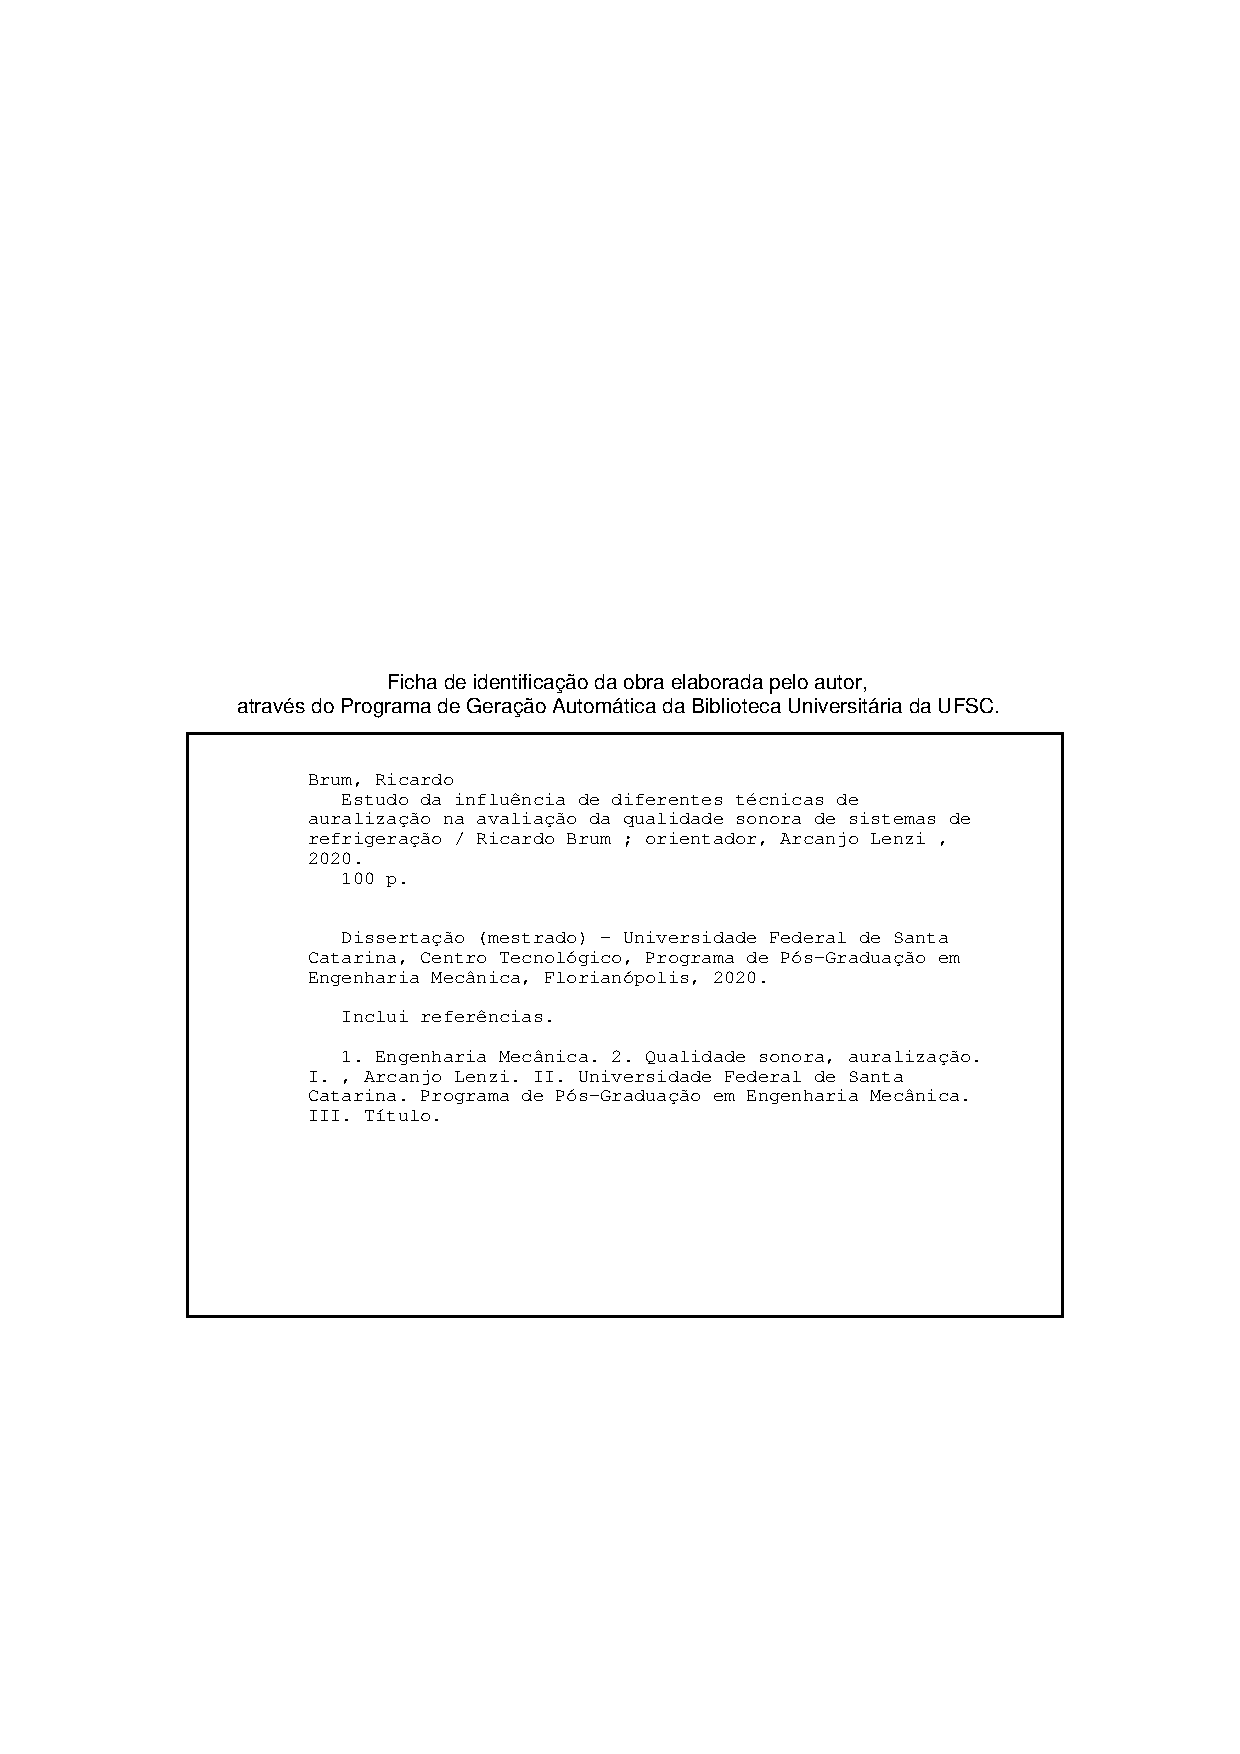
\includepdf{beforetext/Ficha_Catalografica.pdf}
\end{fichacatalografica}
% ---

% ---
% Inserir folha de aprovação
% ---
\begin{folhadeaprovacao}
	\OnehalfSpacing
	\centering
	\imprimirautor\\%
	\vspace*{10pt}		
	\textbf{\imprimirtitulo}%
	\ifnotempty{\imprimirsubtitulo}{:~\imprimirsubtitulo}\\%
	%		\vspace*{31.5pt}%3\baselineskip
	\vspace*{\baselineskip}
	%\begin{minipage}{\textwidth}
	O presente trabalho em nível de \imprimirnivel~foi avaliado e aprovado por banca examinadora composta pelos seguintes membros:\\
	%\end{minipage}%
% 	AQUI VAI A BANCA
% 	\vspace*{\baselineskip}
% 	Ricardo Mikio Doi, Dr.\\
% 	Embraco\\
% 	\vspace*{\baselineskip}
% 	Prof. Bruno Sanches Masiero, Dr.\\
% 	Universidade Estadual de Campinas\\
% 	\vspace*{\baselineskip}
% 	Prof. Erasmo Felipe Vergara Miranda, Dr.\\
% 	Universidade Federal de Santa Catarina\\

	\vspace*{2\baselineskip}
	\begin{minipage}{\textwidth}
		Certificamos que esta é a \textbf{versão original e final} do trabalho de conclusão que foi julgado adequado para obtenção do título de \imprimirformacao.\\
	\end{minipage}
	%    \vspace{-0.7cm}
	\vspace*{\fill}
	\assinatura{\OnehalfSpacing\imprimircoordenador \\ \imprimircoordenadorRotulo~do Programa}
	\vspace*{\fill}
	\assinatura{\OnehalfSpacing\imprimirorientador \\ \imprimirorientadorRotulo}
	%	\ifnotempty{\imprimircoorientador}{
	%	\assinatura{\imprimircoorientador \\ \imprimircoorientadorRotulo \\
	%		\imprimirinstituicao~--~\imprimirinstituicaosigla}
	%	}
	% \newpage
	\vspace*{\fill}
	\imprimirlocal, \imprimirdata.
\end{folhadeaprovacao}
% ---

% ---
% Dedicatória
% ---
\begin{dedicatoria}
	\vspace*{\fill}
	\noindent
	\begin{adjustwidth*}{}{5.5cm} 
		\raggedleft       
% 		A todos os grandes gênios que fizeram da ciência e da arte o centro de suas vidas.
	\end{adjustwidth*}
\end{dedicatoria}
% ---

% ---
% Agradecimentos
% ---
\begin{agradecimentos}
	
\end{agradecimentos}
% ---

% ---
% Epígrafe
% ---
\begin{epigrafe}
	\vspace*{\fill}
	\begin{flushright}
% 		\textit{``Conheça todas as teorias, domine todas as técnicas, mas ao tocar uma alma humana, seja apenas outra alma humana.''\\
% 			(Carl Gustav Jung)}
	\end{flushright}
\end{epigrafe}
% ---

% ---
% RESUMOS
% ---

% resumo em português
\setlength{\absparsep}{18pt} % ajusta o espaçamento dos parágrafos do resumo
\begin{resumo}
	\SingleSpacing
	apresentar rapidamente os objetivos, justificativa, uma ideia da metodologia (citar redes usadas) e resultados
	\textbf{Palavras-chave}: 
\end{resumo}

% resumo em inglês
\begin{resumo}[Abstract]
	\SingleSpacing
	\begin{otherlanguage*}{english}
		
		\textbf{Keywords}: 
	\end{otherlanguage*}
\end{resumo}

{%hidelinks
	\hypersetup{hidelinks}
	% ---
	% inserir lista de ilustrações
	% ---
	\pdfbookmark[0]{\listfigurename}{lof}
	\listoffigures*
	\cleardoublepage
	% ---
	
	% ---
	% inserir lista de quadros
	% ---
	\pdfbookmark[0]{\listofquadrosname}{loq}
	%\listofquadros*
	\cleardoublepage
	% ---
	
	% ---
	% inserir lista de tabelas
	% ---
	\pdfbookmark[0]{\listtablename}{lot}
	%\listoftables*
	\cleardoublepage
	% ---
	
	% ---
	% inserir lista de abreviaturas e siglas (devem ser declarados no preambulo)
	% ---
	\imprimirlistadesiglas
	% ---
	
	% ---
	% inserir lista de símbolos (devem ser declarados no preambulo)
	% ---
	\imprimirlistadesimbolos
	% ---
	
	% ---
	% inserir o sumario
	% ---
	\pdfbookmark[0]{\contentsname}{toc}
	\tableofcontents*
	\cleardoublepage
	
}%hidelinks
% ---


% ---

% ----------------------------------------------------------
% ELEMENTOS TEXTUAIS
% ----------------------------------------------------------
\textual

% ---
% 1 - Introdução
% ---
% ----------------------------------------------------------
\chapter{Introdução} \label{cha:introduction}
% ----------------------------------------------------------

    Os padrões sonoros permitem identificar características importantes do comportamento de sistemas dinâmicos possibilitando ao ser humano reconhecer os mais variados fenômenos. Com as habilidades auditivas e vocais, um individuo é capaz de gerar e discernir sinais sonoros sem significados, fonemas, palavra, frases, e até em uma conversa conseguir encontrar o local de origem de um locutor pelo seu sotaque e regionalismos. Também é possível criar sons com ritmos, timbres, estilos diferentes assimilando assim sues contrastes. Essa capacidade também pode ser utilizada para dar significado a alertas sonoros, ruídos causados por animais, batidas, entre outros. 
    
    As aptidões humanas de classificação de sinais foram relevantes no seu desenvolvimento e na forma de interagir com o mundo  \cite{jung2020human}. Logo, as descrição de comportamento de sistemas são estudadas para desenvolver técnicas que possibilitam aperfeiçoar ou adicionar recursos em produtos e serviços, como também orientar a criação de ferramentas e a detecção de problemas. A identificação de falhas ou condições atípicas de operação em máquinas é uma aplicação interessante \cite{yang2019machine}, pois pode ser verificada diariamente nos produtos, por exemplo, ruídos incomuns produzido por automóveis podem avisar o próprio condutor ou mecânico de algum tipo de problema. Logo, alguns sinais relatam tanto a alertas de avaria como também da qualidade do dispositivo.

    No contexto industrial, essas ferramentas podem ser de grande utilidade para prever falhas tanto nas máquinas da linha de fabricação \cite{purohit2019mimii} quanto no produto final \cite{yang2019machine}, elas auxiliam no desenvolvimento de equipamento em baixo custos de forma automatizada e otimizada \cite{zahid2015optimized}. Outra prática relevante é no monitoramento a partir de sistemas embarcados, o que é vantajoso em situações de grande prejuízo caso a falha no equipamento não seja detectada imediatamente. Nestes casos, o interessante é obter uma análise prévia, se não imediata do problema, para uma abordagem simples e efetiva, gerando menos perda de material e tempo.

    % No contexto industrial, essas técnicas podem ser aplicadas nas produções em série, auxiliando no reconhecimento de mau funcionamento nas linhas. Essas ferramentas são automatizadas para a fabricação de equipamento em baixo custos e otimizada, portanto, outra prática relevante é o monitoramento a partir de sistemas embarcados, o que é vantajoso em situações de grande prejuízo caso a falha no equipamento não seja detectada imediatamente. Nestes casos, o interessante é obter uma análise prévia, se não imediata do problema, para uma abordagem simples e efetiva, gerando menos perda de material e tempo.
    
    % as orientações de conserto são aplicáveis em série, assim como as de reconhecimento de mau funcionamento nas linhas de produção.
    
    Do ponto de vista técnico, a classificação consiste em extrair características tanto físicas quanto perceptivas de um sinal sonoro e, a partir disso, definir uma classe na qual o evento em questão melhor se enquadra \cite{alias2016review}. Para isso, pode-se utilizar algoritmos de extração e classificação de recursos que são bastante diversificados. Uma forma de simplificar essa escolha é ter em mente que ela depende do domínio no qual a análise será realizada. 
    
    Atualmente, novos métodos estão sendo estudados, entre eles a classificação automática de sinais sonoros utilizando \gls{AI}\footnote{Acrônimo do inglês para \ai.}. Essa é uma área crescente de pesquisa com inúmeras aplicações no mundo real existindo uma grande quantidade de trabalhos em campos relacionados ao áudio\cite{unknown}, como fala \cite{abdel2014convolutional} e música \cite{boddapati2017classifying}, e alguns trabalhos sobre a classificação de sons ambientais \cite{boddapati2017classifying}. O conteúdo desses estudos são empregados em produtos e serviços tais como: aplicativos de reconhecimento de fala ou musica, assistente residenciais, próteses auditivas, sistemas de automatização, carros, entre outros. 
    
    É importante averiguar essas tecnologias emergentes tanto no sentido de inovação de produtos quanto na análise preditiva para detecção de prováveis avarias de amostras. Uma aplicação que ainda carece de estudos aprofundados é a classificação de padrões sonoros de compressores hermético utilizando algoritmos de inteligência artificial.
    
    O compressor é um dos responsável pela circulação de fluído ao longo do sistema de refrigeração junto com o condensador, válvula de expansão e evaporador, este dispositivo torna possível o ciclo de refrigeração \cite{boabaid2017estudo}. Ele também é uma das fonte sonoras mais importantes desse conjunto, pois as energias acústicas e vibratórias produzidas no seu interior são transmitidas dele ao ambiente com níveis de ruído consideráveis. Dessa forma, identificar os ruídos anômalos dos típicos é de suma importância para indicar falhas de operação ou descrever a qualidade sonora do produto final.
    
    Portanto, de todos os padrões sonoros de compressores herméticos, foram escolhidos alguns para treinar redes neurais para classifica-los. Essa será uma primeira análise para que em trabalho futuros seja possível reconhecer anomalias no sistema. Entre os sons escolhidos estão: \textit{dripping} (gotejamento), \textit{knock}, \textit{start stop}, batida de mola, operação estacionária.\\
    
    NO FINAL DO TRABALHO VOLTAR PARA DESCREVER TODOS OS SINAIS ESCOLHIDOS.
    
    \section{Objetivos}    
    
        A partir do exposto anteriormente e da necessidade de identificar padrões sonoros de compressores,  o objetivo geral deste trabalho é determinar a eficácia diferentes algoritmos de inteligência artificial para reconhecer e classificar padrões de falhas a partir de sinais pressão produzidos por compressores herméticos de sistemas de refrigeração.
    
    \subsubsection*{Objetivos específicos}
    
        \begin{itemize}
            \item Investigar o funcionamento de diferentes algoritmos de redes neurais para detecção de padrões em sinais de sistemas de refrigeração;
            \item Implementar rotinas de treinamento e classificação de maneira organizada e intuitiva para utilização posterior do \gls{LVA} e empresas parceiras;
            \item Investigar o comportamento dos algoritmos com diferentes tipos de entradas, tais como sinais de pressão sonora e aceleração.
        \end{itemize}
        
    \section{Organização do trabalho}
        
        A estrutura de trabalho está organizada da seguinte forma, há (TANTOS) capítulos. O primeiro é uma introdução dos trabalho de padrão sonoros, das áreas que são beneficiadas por estas técnicas e do motivo de utilizar algoritmos de inteligência artificial para classificar em classes sinais sonoros de compressores.
    
        No Capítulo 2 é apresentado o referencial teórico, no qual são descritas as principais teorias utilizadas para o trabalho, tendo como base  a literatura e as normas referentes a cada área necessária para o desenvolvimento do trabalho.\\
        
        % QUANDO TERMINAR OS OUTROS CAPÍTULOS ESCREVER O RESTO.


% \section*{[Contextualização (só para marcar)]}
% \section*{[Justificativa do trabalho (só para marcar)]}
% \section*{[Proposta do trabalho (só para marcar )]}
% \section{Objetivos}
% \subsection{Objetivo Geral}
% \subsection{Objetivos Específicos}
% \section{Organização do trabalho}
% \section*{Esqueleto do trabalho}
% \begin{enumerate}
%     \item Introdução
%     \begin{enumerate}
%         \begin{enumerate}[label=\theenumi\arabic*]
%             \item[] Contextualização
%             \item[] Justificativa
%             \item[] Proposta
%             \item Objetivos
%             \item Organização do trabalho
%         \end{enumerate}
%     \end{enumerate}
%     \item Fundamentação teórica
%     \begin{enumerate}[label=\theenumi.\arabic*]
%         \item Sinais
%         \begin{itemize}
%             \item Por enquanto os sinais são: operação estacionária, dripping, knock 
%             \item o que se espera dos sinais avaliados (tempo, freq., e da análise energética)
%         \end{itemize}
%         \item PDS
%         \begin{itemize}
%             \item Redução de ruído e SNR
%             \item truncamento de sinais (janelamento)
%             \item Energia do sinal (STFT, mel, mfcc, chroma, spectral contrast, tonnetz)
%         \end{itemize}
%         \item Redes Neurais
%         \begin{itemize}
%             \item Resumo inteligência artificial, aprendizado de maquinas e aprendizado profundo
%             \item Rede convolucional (1D e 2D)
%             \item Rede recorrente (LSTM)
%             \item Rede nn
%             \item Parâmetros de ativação, propagação de erro, etc
%             \item Métricas para avaliação das redes neurais
%         \end{itemize}
%     \end{enumerate}
%     \item Processamento dos sinais e configurações das redes neurais 
%     \begin{enumerate}[label=\theenumi.\arabic*]
%         \item Medição operação estacionária (florinda, condição atmsf, ... )
%         \item PDS - como foi realizado:
%         \begin{itemize}
%             \item criação do banco de dados
%             \item redução de ruído
%             \item SNR
%             \item concatenação dos sinais
%             \item os cortes (se descaracterizar)
%             \item nº de amostras
%             \item calculo de energia dos sinais
%             \item determinação das features
%         \end{itemize}
%         \item Treinamento das redes neurais
%         \begin{itemize}
%             \item determinação dos labels
%             \item reshape dos sinais para input na rede
%             \item separação do sinais (traino, validação e teste)
%             \item configuração das redes (métricas, breakpoints, endpoints, ...)
%             \item como foi implementada as redes neurais (cnn, cnn2d, nn e LSTM)
%         \end{itemize}
%     \end{enumerate}
%     \item Resultados do banco de dados teste (atualmente os resultados que tenho - para as 4 redes analisadas)
%     \begin{enumerate}[label=\theenumi.\arabic*]
%         \item Configuração sinais de entrada: 1340 amostras de 1 s cada
%         \begin{itemize}
%             \item sinais individuais de dripping, knock e op. estacionária sem alteração na SNR
%             \item sinais concatenados (fenômenos a op. estacionária + op. estacionária individual) sem alteração na SNR
%             \item sinais concatenados (fenômenos a op. estacionária) sem alteração na SNR
%             \item sinais concatenados (fenômenos a op. estacionária) com alteração na SNR (-6 e -12 dBFS)
%         \end{itemize}
%         \item Configuração sinais de entrada: 16 e 32 amostras de 1 s cada
%         \begin{itemize}
%             \item sinais concatenados (fenômenos a op. estacionária) com alteração na SNR (-6 e -12 dBFS)
%         \end{itemize}
%         \item Configuração sinais de entrada: 16 e 32 amostras de 0.2 s cada
%         \begin{itemize}
%             \item sinais concatenados (fenômenos a op. estacionária) com alteração na SNR (-6 e -12 dBFS)
%         \end{itemize}
%     \end{enumerate}
%     \item Considerações finais
% \end{enumerate}

% ----------------------------------------------------------
\chapter{Fundamentação teórica}\label{cap:fundteo}
% ----------------------------------------------------------
    Neste capítulo serão abordados os principais aspectos teóricos utilizados neste trabalho.

    \section{Diferença entre \ia, \am e \ap}
    
        Os temas \ia, \gls{ML}\footnote{Acrônimo do inglês para \ml.} e \gls{DL}\footnote{Acrônimo do inglês para \dl.} são discutidos assiduamente em estudos e vendidos como diferencial de produtos. Portanto nesta seção será definida cada uma dessas áreas e subáreas, apresentando suas diferenças. %nos meios de comunicação,
    
        A \ia, se propõe elaborar dispositivos que simulem a capacidade humana de raciocinar, perceber, tomar decisões e resolver problemas. Logo, qualquer técnica que permita computadores simular o comportamento humano pode ser definida com uma AI \cite{DeepLearningArtigo}. 
    
        \am é um subárea de AI. Seu intuito é fazer que as máquinas aprendam sozinhas usando dados fornecidos e assim, consigam realizar previsões com uma dada incerteza. Dentre os algorítimos de ML existe um outro subconjunto conhecido como \ap\textit{ }focado em \gls{NN}\footnote{Acrônimo do inglês para \nn.} \cite{kim2017matlab} .  
        
        As \rns\textit{ }são uma forma de modelar matematicamente sistemas de neurônios biológicos, e utiliza-los para resolver tarefas que outros tipos de algoritmos não conseguem realizar, por exemplo, classificação de imagens. Os subconjuntos de que compõem a AI podem ser visualizados na Figura~\ref{fig:AI_Ml_DL}.
            
        \begin{figure}[H]
            \centering
            \caption{Esquemático dos subconjuntos da AI.}
            \includegraphics[width=0.7\textwidth]{fig/2-fundamentacao/diferenca_AI_ML_DL/Areas.png}
            \fonte{adaptado de \cite{site:RevolucaoIA}.}
            \label{fig:AI_Ml_DL}
        \end{figure}
        
        A ideia de \ap\textit{ }ser um "tipo"\textit{ }de \am\textit{ }é muito importante, e este é o motivo de realizar uma revisão sobre como AI, ML e DL estão relacionados. O \ap, por ter resolvido com proficiência alguns problemas que desafiaram a \ia\textit{ }esta em destaque recentemente. Seu desempenho, a pesar de ser excepcional em muitos campos, também enfrenta limitações que derivam de seus conceitos fundamentais os quais foram herdados de seu antecessor o ML. Como uma subárea do aprendizado de máquina, o aprendizado profundo não pode evitar os problemas base que o ML enfrenta. Por isso que é necessário apresentar o \am\textit{ }antes de discutir o conceito de \ap, o que será feito na seção~\ref{cap:ML}, porque o ML é alicerce do DL. 
        
    \section{Aprendizado de Máquinas}\label{cap:ML}
        
        Uma outra forma de compreender as técnicas de \am, é entendê-lo como método de análise de dados que visa automatizar a construção de modelos analíticos. Seus algoritmos são capazes de aprender iterativamente com os dados, possibilitando que computadores encontrem \textit{insights} sem serem explicitamente programados sobre onde e o que procurar nas informações \cite{CollegeL30:online}.
        
        Posto isso, nesta seção serão apresentadas as terminologias básicas necessárias em \am, como se dá o aprendizado e de que forma seus erros são reduzidos. Também será discutida a diferença entre tarefas supervisionadas e não supervisionadas, assim como a distinção entre classificação e regressão. No final, serão descritas as métricas de avaliação de performance de modelos de classificação.
        
        \subsection{Terminologias Fundamentais de ML e Introdução a Conceitos Básicos}
        
            Nesta subseção serão definidas terminologias fundamentais de \am e \ap obtidas em \cite{MachineL6:online}. A partir disso, é possível determinar conceitos como: tipos de tarefas, diferenças entre treinamento e inferência e assim por diante.
    
            Há dois tipos de tarefas em \am, as supervisionadas e as não supervisionadas. As tarefas supervisionadas aprendem como a combinar inputs para produzir previsões úteis sobre dados nunca antes vistos, ou seja, se tem conhecimento sobre qual é a saída para uma dada entrada \cite{singh2016review}. Já no caso de não ter noção prévia do que espera-se como inferência das redes, utiliza-se modelos não supervisionados.
        
            Duas terminologias muito importantes em \am\textit{ }supervisionada são os rótulos\footnote{Em inglês \textit{labels}.} e os atributos\footnote{Em inglês \textit{features}.} ). Os rótulos, são as classes e também o que se espera como predição do modelo, representado pela variável $y$. As atributos, são as variáveis de entrada (valores que caracterizam as amostras), representado por $x$. 
            
            Uma das formas de indicar o quão sofisticado é um projeto de aprendizado de máquinas é através da quantidade de atributos. Ou seja, redes que recebem como entradas poucos recursos são mais simples que as com múltiplas entradas. 
            
            Do conjunto de amostras, um exemplos é uma instância particular de dados do vetor de atributos $\mathbf{\overline{x}}$ e são classificados em duas categorias: exemplo rotulado\footnote{Em inglês \textit{labeled examples}.} e exemplo não rotulado\footnote{Em inglês \textit{unlabeled examples}.}. 
            
            Um exemplos rotulados incluí tanto atributo(s) como o rótulo(s). Ou seja:
            \begin{center}
                exemplos rotulados: \{atributo, rótulo\}: (x, y)
            \end{center}
    
            Já um exemplos não rotulados contem apenas as atributo(s) sem o rótulo(s). Como representado a seguir:
            \begin{center}
                exemplos não rotulados: \{atributo, ?\}: (x, ?)
            \end{center}
    
            Os problemas mais comuns resolvidos com este tipo de ML são os de regressão e classificação. Uma diferença entre eles, é que a regressão prediz valores contínuos, enquanto a classificação prediz valores discretos. Outra característica importante ocorre na forma de avaliar performance, com métricas específicas para cada um. Elas serão descritas na seção~\ref{cap:metrica}. 
            
            De tudo o que foi exposto até agora, é possível concluir que modelos de classificação e regressão necessitam de um banco de dados prévio, visto que utilizam exemplos com e sem rótulos, ou seja, são tarefas supervisionadas. Já no caso de aprendizado não supervisionado, que não se sabe a saída, exemplos comuns de aplicação são: problemas como detecção de anomalias (não se tem conhecimento do problema); agrupamentos individuais \footnote{Em inglês \textit{cluster}.}; e redução de dimensionalidade \cite{gentleman2008unsupervised}. Como este trabalho será sobre classificação de padrões sonoros, as técnicas de aprendizado supervisionado não serão abordadas.
            
            Para finalizar as definições básicas, necessita-se determinar o que é modelo, isso do ponto de vista de tarefas supervisionadas. Ele tem duas fases, que são:
    
            \begin{itemize}
                \item Treinamento: fase na qual o modelo aprende, ou seja, ele receberá exemplos rotulados e será permitido que ele gradualmente encontre a relação entre $x$ e $y$;
                \item Inferência: momento que será aplicado o modelo treinado em exemplos não rotulados, isto é, ele faz predições uteis ($y'$).
            \end{itemize}
    
    
        \subsection{Treinando modelo simples para compreender \am}\label{cap:ML_modelo_qualquer}
            
            A Figura~\ref{fig:dados_quaisquer} apresenta uma pequena amostra de dados observados, e a partir delas deseja-se encontrar uma relação entre $y$, variável de interesse dependente que se quer predizer, e $x$ a variável independente.
            
            \begin{figure}[H]
                \centering
                \caption{Pequena amostra de dados quaisquer.}
                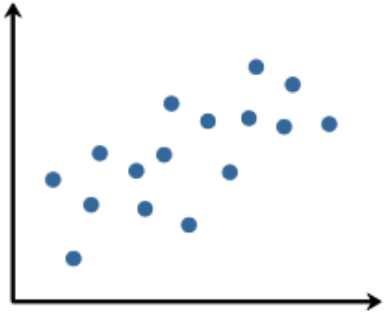
\includegraphics[width=0.3\textwidth]{fig/2-fundamentacao/treinar_modelo_simples/dados_quaisquer.png}
                \fonte{\cite{MachineL6:online}}
                \label{fig:dados_quaisquer}
            \end{figure}
            
            Pela análise da Figura~\ref{fig:dados_quaisquer} é possível dizer que, uma reta consegue inferir o comportamento entre $x$ e $y$, mesmo que não passe exatamente por todos os pontos, como a Figura~\ref{fig:dados_quaisquer_regressao} demonstra. Matematicamente é descrita pela equação~\ref{eq:reta} na convenção estabelecida em ML e adicionando o subíndice que indica a possibilidade de ter mais de uma dimensão. Para inferir $y$, basta substituir os valores de $x$ neste modelo (reta) \cite{CollegeL30:online}.
            
            \begin{equation}\label{eq:reta}
                \centering
                y' = b + w_{1}x_{1};
            \end{equation}
        
            em que:
            \begin{itemize}
                \item $y'$ é o rótulo predito \footnote{Em inglês \textit{predicted label}.} (saída desejado);
                \item $b$ é o bias (intercepção no eixo $y$);
                \item $w_{1}$ é o peso da atributo 1. Peso tem o mesmo conceito que a inclinação ($m$) tem na equação tradicional da reta;
                \item $x$ é o atributo (entrada).
            \end{itemize}
    
            \begin{figure}[H]
                \centering
                \caption{Regressão linear que prever o comportamento da pequena amostra de dados quaisquer.}
                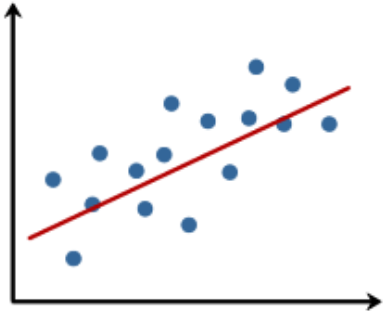
\includegraphics[width=0.3\textwidth]{fig/2-fundamentacao/treinar_modelo_simples/dados_quaisquer_regrassao.png}
                \fonte{\cite{MachineL6:online}}
                \label{fig:dados_quaisquer_regressao}
            \end{figure}
            
            O exemplo proposto considerar somente uma dimensão de atributos como entrada, ao contrário de modelo mais sofisticado que utilizam muito mais, e com isso, possuem mais pesos ($w$). Logo, há um peso para cada atributo em separado, como descreve a equação~\ref{eq:reta_varias_features}. 
            
            \begin{equation}
                \centering
                y' =  b + w_{1}x_{1} + w_{2}x_{2} + ... + w_{n}x_{n}.
                \label{eq:reta_varias_features}
            \end{equation}
            
            Para sintetizar, os dados foram aplicados em um algoritmo de \am e como resultado obteve-se um modelo, que neste caso é uma reta. Mas é gerada uma a pergunta: como o treinamento realmente acontece? Ele ocorre ao determinar bons valores para o bias e todos os pesos utilizando exemplos rotulados. Para isso, o algoritmo examina varias amostras, e compara a predição feita pela equação criada, com o valor real, buscando encontrar um modelo que minimize a perda entre $y$ e $y'$.
            
            A perda é também conhecida como erro, que é dado por um número que indica o quão boa foi a inferência de um exemplo único. Ele pode ser visto como uma penalidade dada ao modelo por fazer uma predição ruim. Se $y'$ for igual a $y$, a perda será zero, caso contrário, será um valor maior que zero e grande. 
            
            A Figura~\ref{fig:loss_learning} apresenta dois modelos, sendo que o da esquerda possui um erro alto. Uma forma de concluir isso, é através da distância muito maior entre a linha azul (equação) e o ponto (valor verdadeiro). No gráfico da direta esse espaço é pequeno, mostrando que a perda é menor.
    
            \begin{figure}[H]
                \centering
                \caption{O gráfico da esquerda ilustrar um modelo com alta perda e o da direita com baixa perda.}
                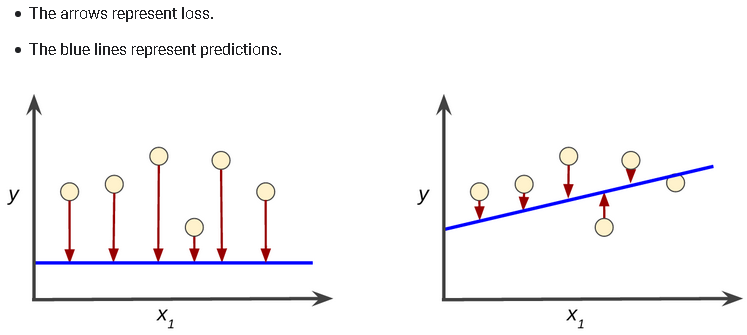
\includegraphics[width=0.7\textwidth]{fig/2-fundamentacao/aprendizado/loss_learning.png}
                \fonte{\cite{MachineL6:online}}
                \label{fig:loss_learning}
            \end{figure}
            
             Portanto o objetivo dos algoritmos de ML e DL é treinar o modelo para encontrar os valores de $w_i$ e $b$ que minimize essa diferença ao longo de todos os exemplos. A equação mais comum usada para esse cálculo é erro quadrático\footnote{Em inglês \textit{squared loss}.} , entretanto, ela é usada a partir do valor médio, denominado \gls{MSE}\footnote{Acrônimo do inglês para \textit{Mean square Error}.}, e descrito pela equação~\ref{eq:MSE}\cite{TotalTen29:online}.
            
            \begin{equation}
                \centering
                MSE =  \frac{1}{N} \sum_{(x,y)\in D}  (y - y')^2
                \label{eq:MSE}
            \end{equation}
        
            
            em que:
            \begin{itemize}
                \item $(x,y)$ é um exemplo no qual
                \begin{itemize}
                    \item $x$ é o conjunto de atributos que o modelo usa para realizar predições;
                    \item $y$ é o rótulo do exemplo.
                \end{itemize}
                \item $y'$ é a função de pesos e bias em combinação com o conjunto de atributos $x$;
                \item $D$ é um conjunto de dados contendo muitos exemplos rotulados, nos quais $(x,y)$ são pares;
                \item $N$ é o número de exemplos em $D$.
            \end{itemize}
            
       \subsection{Redução de Perda}     
    
            O diagrama apresentado na Figura~\ref{fig:abordagem_iterativa}, demonstra como o modelo de aprendizado de máquina reduz a perda iterativamente para aprender. Esse processo começa com o algoritmo gerando um "palpite", ou seja, um valor para $b$ e $w_1$. Então, o erro é calculado através da equação~\ref{eq:MSE}. 
            
            As entradas, na estimativa da perda, são o conjunto de rótulos, $y$, e a inferência, $y'$, realizada pelo primeiro modelo utilizando o conjunto de atributos. Após é repetido este processo, entretanto com um novo palpite e da comparação entre os resultado obtidos, o algoritmo escolhe qual das tentativa obteve o menor erro.
    
            \begin{figure}[H]
                \centering
                \caption{Abordagem iterativa para o treinamento do modelo através da redução do erro.}
                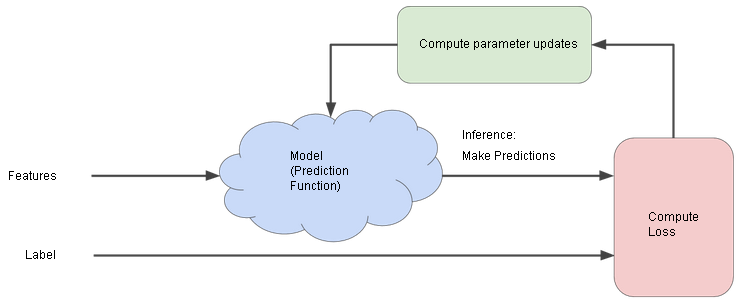
\includegraphics[width=0.8\textwidth]{fig/2-fundamentacao/aprendizado/abordagem_iterativa.png}
                \fonte{\cite{MachineL6:online}}
                \label{fig:abordagem_iterativa}
            \end{figure}
            
            O diagrama~\ref{fig:abordagem_iterativa} tem uma etapa chamada de \textit{Compute Loss}, que representa o momento no qual o algoritmo determina o erro. Na sequência, há o processo \textit{Compute Parameter Updates}, que caracteriza a rede e examina os valores calculados pela função de perda e escolhe como será a atualização deles. Esse procedimento de aprendizado continua a cada iteração até que o algoritmo descubra os parâmetros do modelo com a menor perda possível. 
            
            O ponto no qual o treinamento é interrompido é denominado ponto de corte, e é estabelecido a partir de um critério de parada. Normalmente determina-se esse momento na época na qual a perda geral para de mudar ou pelo menos mude de forma extremamente lenta, quando isso acontece, o modelo convergiu.
            
            Foi usado como exemplo um modelo de regressão linear, se para este caso forem calculados todos os valores possíveis de perda para $w_1$, o resultado seria sempre uma parábola com concavidade para cima. Ela é apresentada no gráfico convexo da Figura~\ref{fig:convexo}.
    
            \begin{figure}[H]
                \centering
                \caption{Problemas de regressão linear geram gráficos de perda vs $w_1$ (peso) convexo.}
                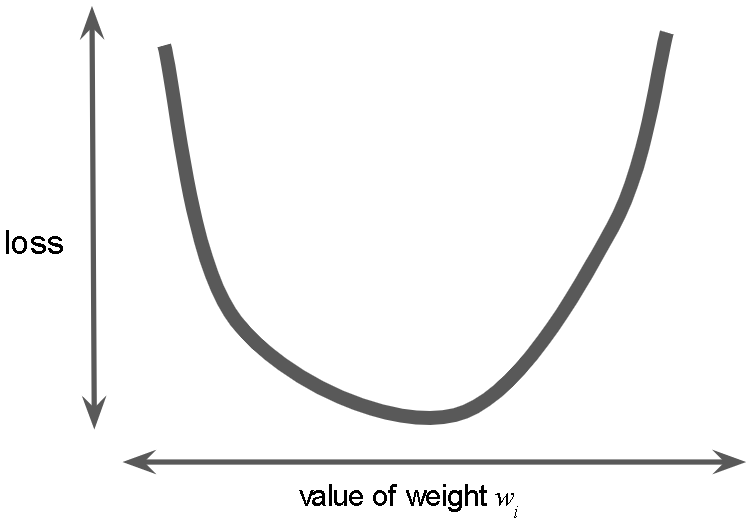
\includegraphics[width=0.435\textwidth]{fig/2-fundamentacao/aprendizado/convexo.png}
                \fonte{\cite{MachineL6:online}}
                \label{fig:convexo}
            \end{figure}
            
            Esse problema é muito simples, pois uma parábola possuí apenas um mínimo, ou seja, um ponto cuja inclinação é exatamente igual a 0. Entretanto, por mais fácil que seja visualizar o ponto onde a função perda converge em uma parábola, ainda é um processo inviável e ineficiente levantar todos os valores para posteriormente encontrar o mínimo.
            
            Um método melhor e mais popular, no aprendizado de máquinas, é o gradiente descendente. Essa técnica também começa com um palpite para $b$ e $w_1$. O ponto de partida não importa muito, assim, muitos algoritmos simplesmente configuram para iniciar em 0 ou em um valor aleatório, como exemplo, a Figura~\ref{fig:gradiente_descendente_ponto_inicial}. 
    
            \begin{figure}[H]
                \centering
                \caption{Ponto de partida aleatório utilizado pelo gradiente descente para minimizar a perda.}
                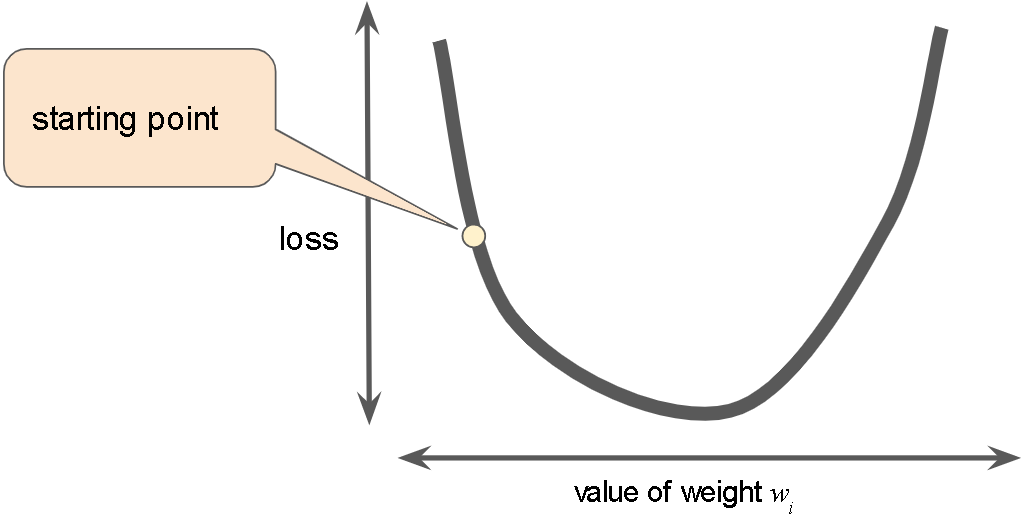
\includegraphics[width=0.6\textwidth]{fig/2-fundamentacao/aprendizado/gradiente_descendente_ponto_inicial.png}
                \fonte{\cite{MachineL6:online}}
                \label{fig:gradiente_descendente_ponto_inicial}
            \end{figure}
            
            O algoritmo calcula o erro no ponto inicial pela derivada parcial, que informa o quanto a função muda quando é feita uma pequena perturbação em uma variável com dado peso. Com base nesta variação, o gradiente consegue predizer se a inclinação da derivada é positiva ou negativa. Como o intuito é encontrar o mínimo, a rede seguirá o gradiente negativo, conhecido como gradiente descendente. Quando há vários pesos, o gradiente é um vetor de derivadas parciais em relação aos pesos. Como o gradiente é um vetor, ele tem uma direção e uma magnitude e seu resultado sempre aponta na direção do gradiente negativo para reduzir a perda o mais rápido possível, como mostra a Figura~\ref{fig:vetor_direcao_gradiente}. 
    
            \begin{figure}[H]
                \centering
                \caption{A descida do gradiente depende de gradientes negativos.}
                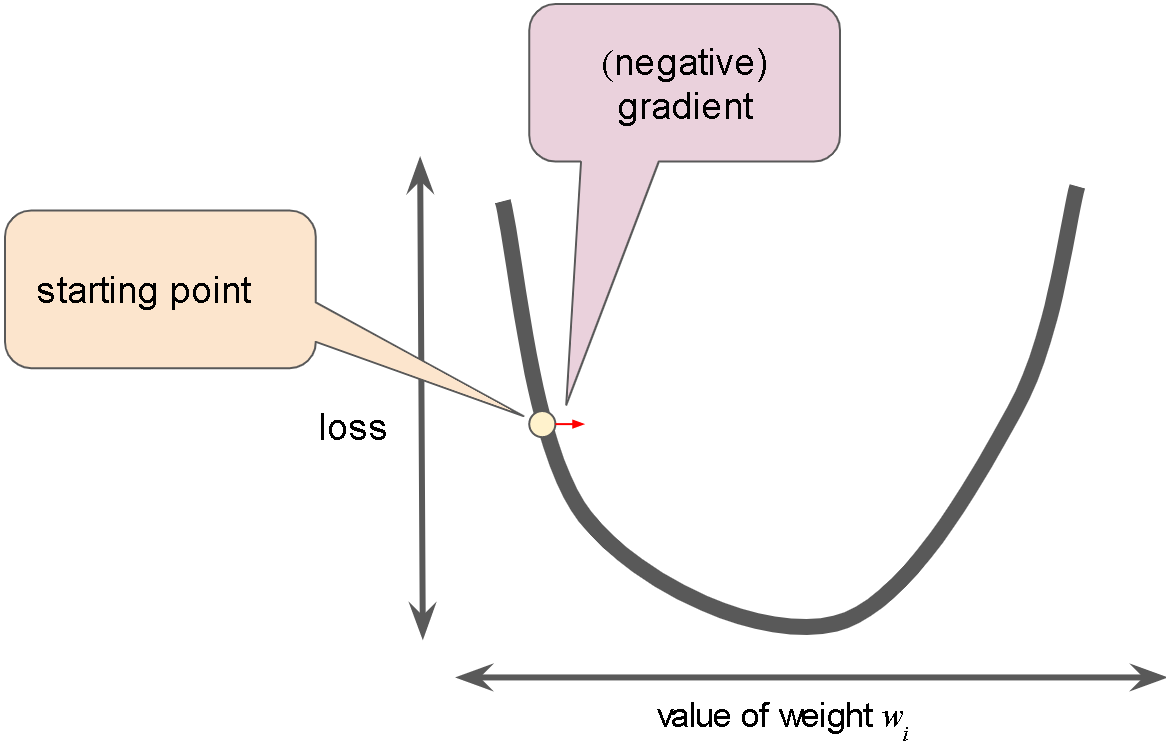
\includegraphics[width=0.6\textwidth]{fig/2-fundamentacao/aprendizado/vetor_direcao_gradiente.png}
                \fonte{\cite{MachineL6:online}}
                \label{fig:vetor_direcao_gradiente}
            \end{figure}
            
            Para determinar o próximo ponto ao longo da curva de perda, o algoritmo adiciona uma fração da magnitude do gradiente ao ponto inicial, conforme mostrado na Figura~\ref{fig:vetor_magnitude_gradiente}. Esse processo é repetido, chegando cada vez mais perto do mínimo. 
    
            \begin{figure}[H]
                \centering
                \caption{Acréscimo da magnitude do gradiente no valor do ponto inicial move para o próximo ponto da curva de perda.}
                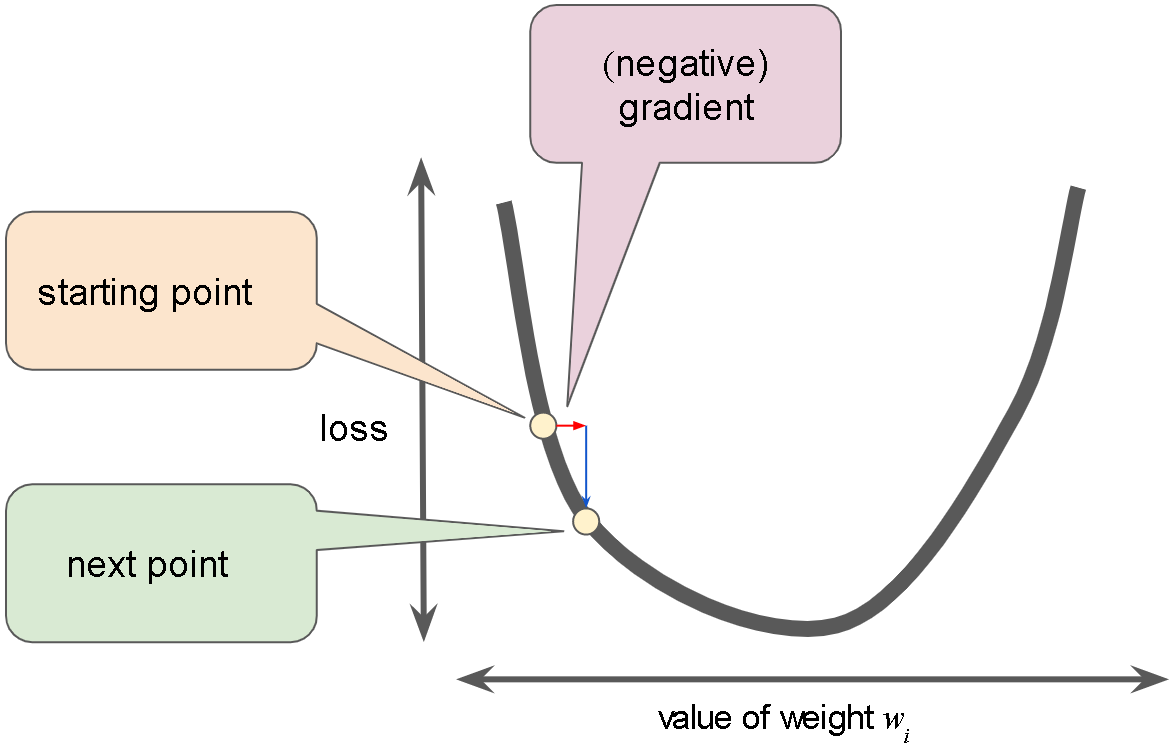
\includegraphics[width=0.6\textwidth]{fig/2-fundamentacao/aprendizado/vetor_magnitude_gradiente.png}
                \fonte{\cite{MachineL6:online}}
                \label{fig:vetor_magnitude_gradiente}
            \end{figure}
            
            Entretanto, não é somente somado ao ponto inicial o valor da magnitude. Antes disso, ela é multiplicada pala taxa de aprendizado, também chamado de tamanho do passo. A taxa de aprendizado é um hiper parâmetro, ou seja, uma das variáveis que controla o próprio processo de treinamento. Esse conjunto soma e multiplicação que realmente dita o próximo ponto de análise na função de perda. Para exemplificar, pode-se considerar uma magnitude de 2,5 e uma taxa de 0,01. O algoritmo escolherá o próximo ponto a uma distancia de 0,025 do valor anterior.
            
            A taxa de aprendizado trás algumas informações importantes: se ela for muito pequena, o treinamento demorará muito como mostra a Figura~\ref{fig:taxa_pequena}. Por outro lado, se ela for muito grande, o ponto irá saltar perpetuamente ao acaso perto do vale sem convergir, demonstrado pela Figura~\ref{fig:taxa_grande}. 
    
            \begin{figure}[H]
                \centering
                \caption{Se a taxa de aprendizagem for muito pequena a proximidade entre os passos é maior.}
                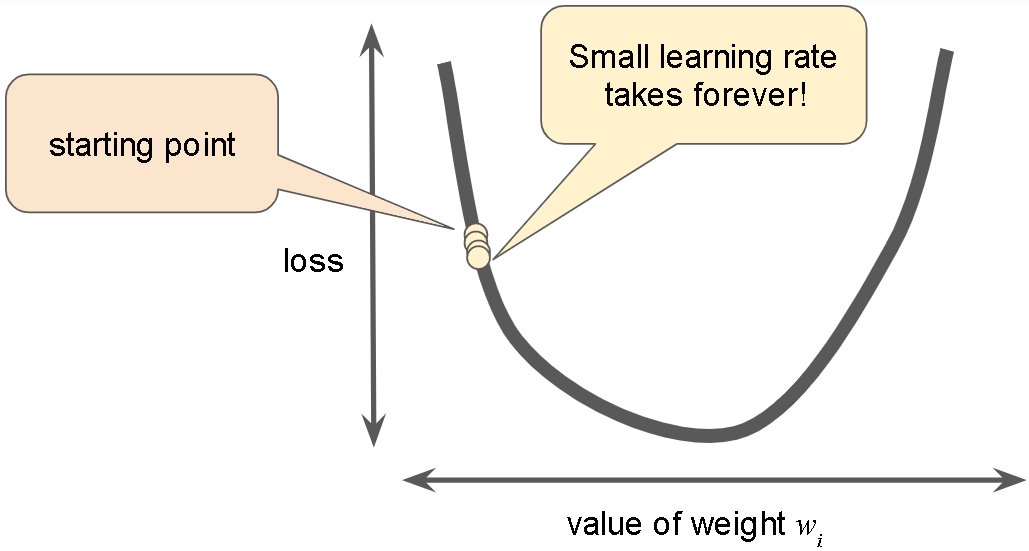
\includegraphics[width=0.6\textwidth]{fig/2-fundamentacao/aprendizado/taxa_pequena.png}
                \fonte{\cite{MachineL6:online}}
                \label{fig:taxa_pequena}
            \end{figure}
            
            \begin{figure}[H]
                \centering
                \caption{A taxa de aprendizagem é muito grande.}
                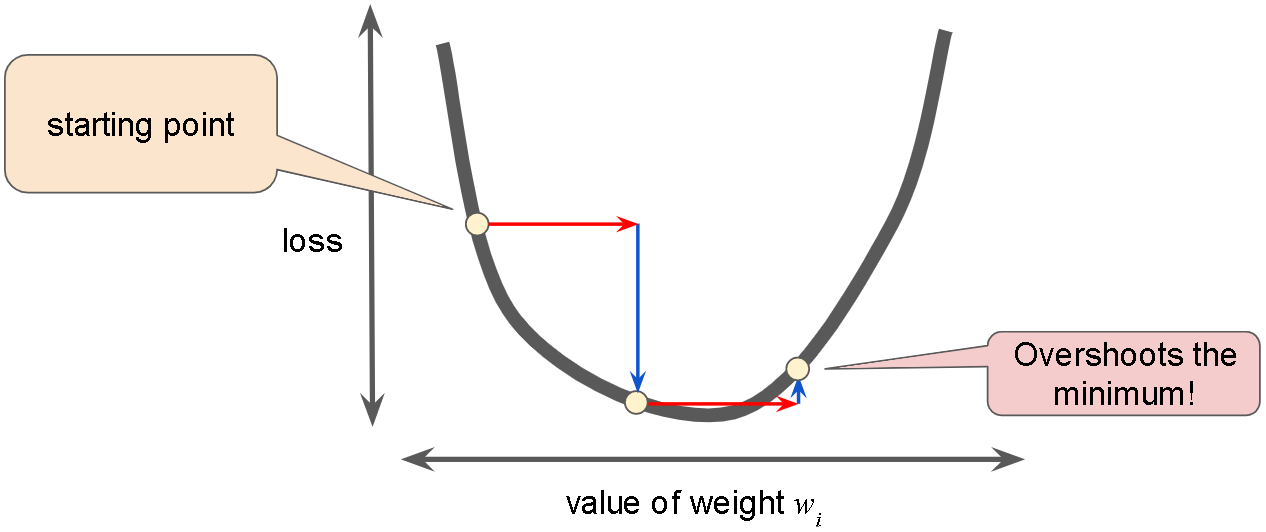
\includegraphics[width=0.6\textwidth]{fig/2-fundamentacao/aprendizado/taxa_grande.png}
                \fonte{\cite{MachineL6:online}}
                \label{fig:taxa_grande}
            \end{figure}
            
            Existe uma taxa de aprendizagem \textit{Goldilocks}\footnote{Em \rns\textit{ }é a taxa de aprendizado ideal.} para cada problema de regressão, que descreve o quão plana é a função de perda. Essa informação permite aumentar com segurança a taxa de aprendizado, se for de conhecimento prévio que o gradiente é pequeno. Com essa compreensão que o valor da magnitude do gradiente é pequeno, é possível configurar um tamanho de passo maior, e dessa forma, que a perda encontre o mínimo no menor número de etapas. Já a taxa de aprendizagem ideal em uma dimensão é o inverso da segunda derivada de $f(x)$ em $x$ e para 2 ou mais dimensões é o inverso da matriz das derivadas parciais secundárias. 
            
            Uma terminologia importante, no gradiente descendente, é lote\footnote{Em inglês \textit{batch}.} definido como o número total de exemplos usados para calcular o gradiente em uma única iteração. Quando é dado como entrada para o cálculo da inclinação o conjunto inteiro de dados, considera-se que foi utilizado um lote. Entretanto, eles geralmente contêm um grande número de atributos, ou seja, um lote pode ser enorme, fazendo com que até mesmo uma única iteração demore muito para ser computada.     
            
        \subsection{Generalização em modelos}
        
            Para descrever o que significa um modelo sobre-ajustado\footnote{Em inglês \textit{overfitting}}, um modelo sub-ajustado\footnote{Em inglês \textit{underfitting}} e o porquê de separar os dados em subconjuntos, serão usadas outras amostras com somente um atributo, apresentadas na Figura~\ref{fig:dados_simples}. Assim como no exemplo da seção anterior~\ref{cap:ML_modelo_qualquer}, o objetivo é desenvolver um modelo para prever os rótulos e a partir dele discutir esses processos \cite{kim2017matlab}.
    
            \begin{figure}[H]
                \centering
                \caption{Pequena amostra de dados com somente uma dimensão atributos.}
                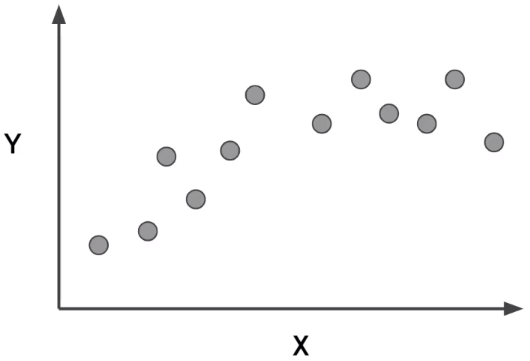
\includegraphics[width=0.5\textwidth]{fig/2-fundamentacao/overfitting/dados_simples.png}
                \fonte{\cite{Complete79:online}}
                \label{fig:dados_simples}
            \end{figure}
    
            É considerado como um bom modelo aquele que tenta se ajustar à tendência geral do conjunto de dados real, e não se encaixar perfeitamente neles. A Figura~\ref{fig:modelo_bom} exibe esse comportamento de generalizar seus resultados.
    
            \begin{figure}[H]
                \centering
                \caption{Comportamento esperado para um bom modelo.}
                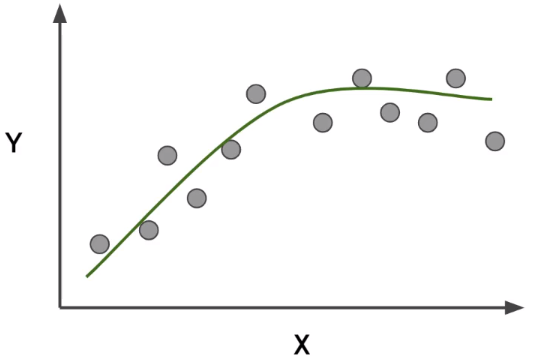
\includegraphics[width=0.5\textwidth]{fig/2-fundamentacao/overfitting/modelo_bom.png}
                \fonte{\cite{Complete79:online}}
                \label{fig:modelo_bom}
            \end{figure}
            
            A Figura~\ref{fig:overfitting} apresenta o comportamento de um  modelo com sobre-ajuste utilizando as amostras da Figura~\ref{fig:dados_simples}. Nela é possível ver que a curva passa exatamente em todos os pontos do gráfico. Quando isso acontece, ele se torna mais complexo do que necessário, seu erro de treinamento é extremamente baixo ou, como neste caso específico, igual à zero.
            
            \begin{figure}[H]
                \centering
                \caption{Modelo considerado ruim com a presença de sobre-ajuste.}
                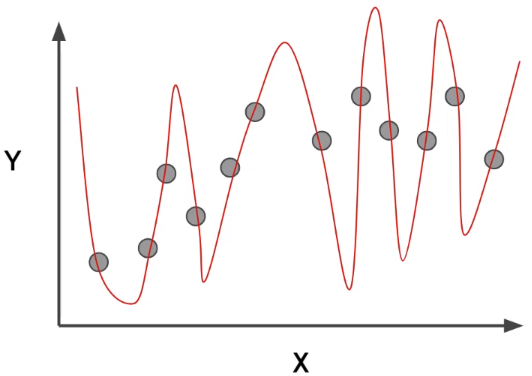
\includegraphics[width=0.5\textwidth]{fig/2-fundamentacao/overfitting/overfitting.png}
                \fonte{\cite{Complete79:online}}
                \label{fig:overfitting}
            \end{figure}
            
            O oposto do sobre-ajuste é o sub-ajuste, que ocorre em modelos excessivamente simples os quais não conseguem capturar a tendência dos dados para prever seu comportamento. Como resultado, frequentemente, apresentam baixa variança e alto bias. Um exemplo é apresentado na Figura~\ref{fig:underfitting}, ele também foi baseados nas amostras da Figura~\ref{fig:dados_simples}.
            
            \begin{figure}[H]
                \centering
                \caption{Exemplo de um modelo considerado ruim por apresentar sub-ajuste.}
                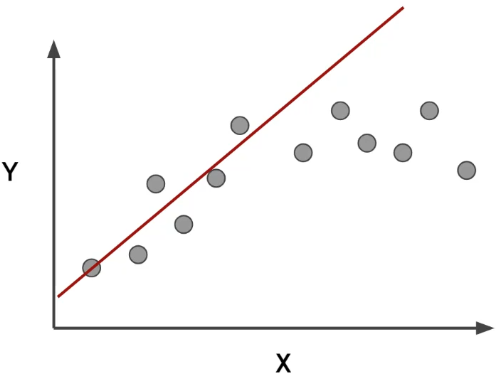
\includegraphics[width=0.5\textwidth]{fig/2-fundamentacao/overfitting/unterfitting.png}
                \fonte{\cite{Complete79:online}}
                \label{fig:underfitting}
            \end{figure}
            
            Infelizmente, o modelo não consegue considerar todas as informações possíveis, uma vez que ele só recebe uma amostra de dados, denominado conjunto de treinamento. Isso acarreta em um problema, se ocorrer sobre-ajuste ou sub-ajuste nos exemplos atuais, como confiar que o modelo também fará boas previsões sobre exemplos nunca antes vistos? Esse é o motivo de separar os conjuntos de dados em mais de um subconjunto. As separações mais utilizadas em ML são:
            
            \begin{itemize}
                \item Em duas divisões denominadas: treino e teste;
                \item Em três divisões denominadas: treino, teste e validação.
                % \item Em quatro divisões denominadas: treino, teste, validação e \textit{deployment}.
            \end{itemize} 
            
            O conjunto de teste deve atender à duas condições: ser grande o suficiente para produzir resultados estatisticamente significativos e ser representativo para o conjunto de dados como um todo. Em outras palavras, não pode ser escolhido um conjunto de teste com características diferentes do conjunto de treinamento. 
            
            Supondo que o conjunto de teste atenda às duas condições anteriores, independente de qual divisão for escolhida, haverá um subconjunto para testar o modelo já treinado. Dessa forma, é possível avaliar se há sobre-ajuste ou sub-ajuste a partir dos resultados do cálculo de erro. Isso porque esse valor será pequeno para o conjunto de treinamento, mas para as novas amostras de teste será muito maior. A Figura~\ref{fig:teste_overfitting_novo_valor} apresenta a um ponto de teste.
    
            \begin{figure}[H]
                \centering
                \caption{Novo valor teste aplicado a um modelo com sobre-ajuste.}
                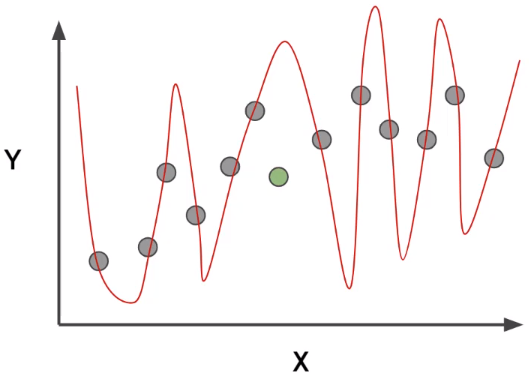
\includegraphics[width=0.5\textwidth]{fig/2-fundamentacao/overfitting/testando_overfitting.png}
                \fonte{\cite{Complete79:online}}
                \label{fig:teste_overfitting_novo_valor}
            \end{figure}
            
            A noção da grandeza do erro pode ser visualizada na distância entre o ponto, valor real, e a curva, equação de inferência, como mostras a Figura~\ref{fig:erro_novo_valor}. Lembrando que, os valores de teste não podem ser utilizados durante o treinamento, garantindo assim, que o modelo não tenha visto antes estes dados.
    
            \begin{figure}[H]
                \centering
                \caption{Apresenta distância entre o novo ponto e a predição do modelo, ou seja, uma visualização do erro.}
                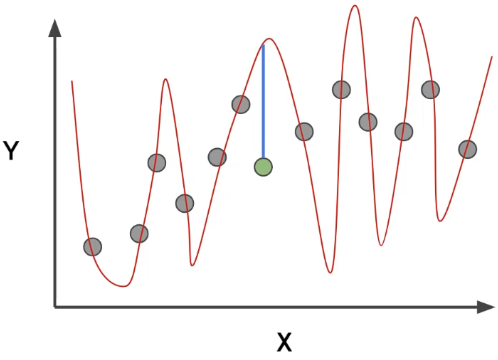
\includegraphics[width=0.5\textwidth]{fig/2-fundamentacao/overfitting/overfitting_erro_evaluate.png}
                \fonte{\cite{Complete79:online}}
                \label{fig:erro_novo_valor}
            \end{figure}
    
            Ao considerar a Figura~\ref{fig:teste_sem_overfitting}, nela esta representado o mesmo o modelo da Figura~\ref{fig:modelo_bom}, considerado bom, e o valor utilizado para teste na Figura~\ref{fig:teste_overfitting_novo_valor}. Por mais que o modelo seja muito simples e que não faça um trabalho perfeito (algumas previsões estão erradas), ele se sai tão bem nos dados de treinamento quanto no ponto de teste, ou seja, a equação não se ajusta demais nos dados de treinamento.
    
            \begin{figure}[H]
                \centering
                \caption{Mostra que a predição do modelo bom não seria perfeita, mas apresentaria um erro menor do que a com sobre-ajuste.}
                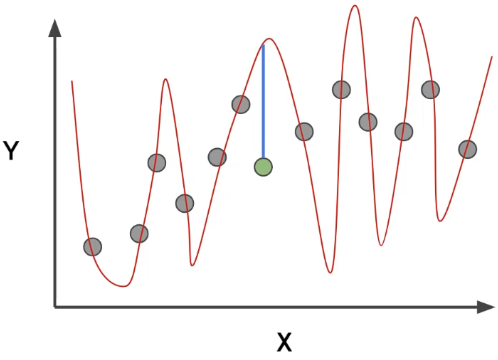
\includegraphics[width=0.5\textwidth]{fig/2-fundamentacao/overfitting/overfitting_erro_evaluate.png}
                \fonte{\cite{Complete79:online}}
                \label{fig:teste_sem_overfitting}
            \end{figure}
            
            Um bom desempenho no conjunto de teste, indica o quanto que se pode confiar nos resultados obtidos com novos dados. Entretanto, isso só é válido se o subconjunto de teste for grande o suficiente; e se não houver "trapaça", isto é, se o mesmo conjunto de teste não for usado repetidamente, ou no lugar do de treinamento. Esse último, pode-se ser concluído por métricas de avaliação com valores surpreendentemente bons, por exemplo, uma alta precisão pode indicar que os dados de teste vazaram para o conjunto de treinamento.
            
            Outra forma de garantir a qualidade dos resultados é eliminando exemplos que acarretam problemas de aprendizado para o algoritmo. Como no caso de um modelo treinado para classificar \textit{e-mails} como sendo spam ou não, o qual as amostras foram distribuídos em treino e teste. Indiferente do resultado, o esperado é obter valores para as métricas menores no conjunto de teste, isso porque o modelo não o usou como base de informações. 
            
            Na hipótese dele atingir a mesma acurácia nos dois conjuntos, treinamento e teste, gera-se um alerta. Logo, os dados devem ser verificados novamente, e se por acaso forem descobertos \textit{e-mail} duplicados entre os dois subconjuntos, a abordagem ideal é remover essas entradas e redividir as amostras. Do contrário, não será possível afirmar o quão bem o modelo consegue se generalizar realizando inferências  corretas sobre novos dados.     
            
            O fluxo de trabalho da divisão em dois conjunto, treino e teste, é ilustrado na Figura~\ref{fig:fluxo_treino_teste}. Nela, a etapa \textit{"Tweak model"} descreve o momento no qual pode-se ajustar a rede, e as possibilidades vão desde alterar a taxa de aprendizado, adicionar ou remover recursos, até projetar um modelo completamente novo do zero. No final deste fluxo de trabalho, escolhe-se o modelo que se sai melhor no conjunto de teste.
    
            \begin{figure}[H]
                \centering
                \caption{Fluxo de trabalho para separação do conjunto de dados em treino e teste.}
                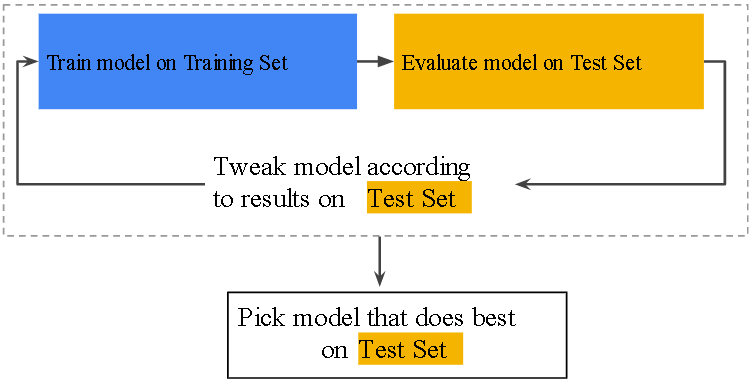
\includegraphics[width=0.7\textwidth]{fig/2-fundamentacao/overfitting/fluxo_treino_teste.png}
                \fonte{\cite{MachineL6:online}}
                \label{fig:fluxo_treino_teste}
            \end{figure}
            
            Entretanto, deve-se observar que esse procedimento é uma abordagem simplificada, pois a divisão é feita somente em dois blocos, o que não é adequado para obter o desempenho final do modelo. Isso porque é possível atualizar os parâmetros repetidas vezes após avaliar os resultados no conjunto de teste. Por causa disso, os dados costumam ser divididos em três conjuntos: treinamento, validação e teste.
            
            Essa abordagem reduz significativamente as chances de ocorrer sobre-ajuste, pois em resumo, as separações das amostra em 3 blocos são usadas da seguinte forma: com o conjunto para o treinamento o modelo consegue aprender as relações entre atributos e rótulos e assim ajustar-se aos dados. As amostras de validação são aplicadas à rede para verificar o desempenho e ele é a referência nos ajuste do modelo (adição de neurônios ou camadas, mudança na arquitetura real da rede etc.). Repete-se esse processo até ter resultados que satisfaçam condições específicas. Só então é possível avaliar a verdadeira performance do modelo com a ajuda da terceira divisão de dados, a de teste. Esse bloco é aplicado em métrica específicas para determinar o comportamento final, esperado em situações práticas. É importante observar que após executar o modelo com os dados de teste não será mais possível voltar e refinar os hiper-parâmetros da rede. O fluxo de trabalho da divisão em três conjunto é ilustrado na Figura~\ref{fig:fluxo_treino_teste_validação}.
    
            \begin{figure}[H]
                \centering
                \caption{Fluxo de trabalho para separação do conjunto de dados em treino, teste e validação.}
                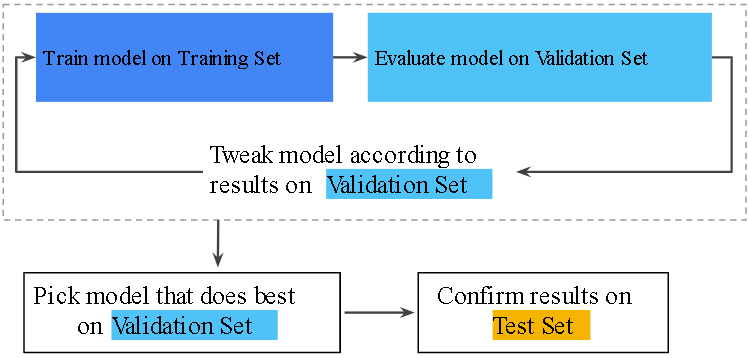
\includegraphics[width=0.7\textwidth]{fig/2-fundamentacao/overfitting/fluxo_treino_teste_validação.png}
                \fonte{\cite{MachineL6:online}}
                \label{fig:fluxo_treino_teste_validação}
            \end{figure}
            
            Até agora, as explicações foram realizadas com base em problemas de uma única atributos, pois são de fácil visualização. Entretanto, isso não ocorre frequentemente em situações práticas, em que a maior parte do tempo, trabalha-se com conjuntos de dados multidimensionais, o que exige uma abordagem diferente. Para discutir o melhor procedimento, pode-se considerar a Figura~\ref{fig:erro_tempo_treinamento} que apresenta a relação entre medição do erro e tempo de treinamento de um modelo considerado ideal.
            
            \begin{figure}[H]
                \centering
                \caption{Modelo ideal em relação ao erro versus tempo de treinamento.}
                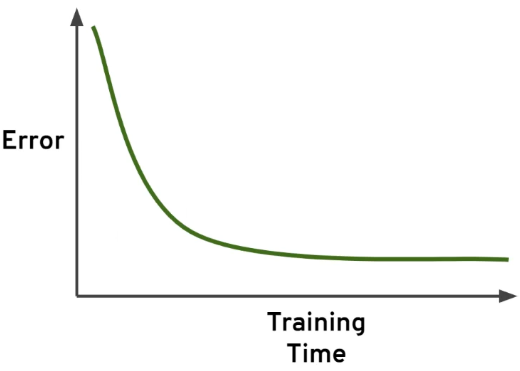
\includegraphics[width=0.5\textwidth]{fig/2-fundamentacao/overfitting/multidimencional_treinamento.png}
                \fonte{}
                \label{fig:erro_tempo_treinamento}
            \end{figure}
            
            Ao aplicar os dados de treinamento pela primeira vez no modelo, o valor de perda obtido será grande. Isso ocorre porque o algoritmo não teve acesso a essas informações antes e não ajustou quaisquer parâmetros internos como hipótese inicial. No entanto, conforme ocorre o aprendizado, ou seja, quanto mais tempo de treinamento, espera-se que o erro diminua até que se estabilize e convergindo para algum tipo de mínimo.
            
            No caso de redes neurais, este tempo de treinamento tem uma denominação específica, época\footnote{Em inglês epochs}. Essencialmente, uma época ocorre quando a totalidade dos dados de treinamento passa pelo modelo. Esse procedimento acontece várias vezes até que se obtém um bom modelo, como mostra a Figura~\ref{fig:epoch}. % erro convergirá para algum tipo de mínimo o
            
            \begin{figure}[H]
                \centering
                \caption{Modelo ideal em relação ao erro versus épocas.}
                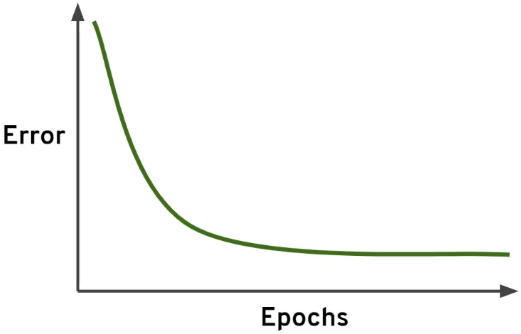
\includegraphics[width=0.5\textwidth]{fig/2-fundamentacao/overfitting/epoch.png}
                \fonte{\cite{Complete79:online}}
                \label{fig:epoch}
            \end{figure}
            
            Um modelo péssimo apresenta erros crescentes a medida que o tempo passa, ou seja, o modelo não aprende a cada época. Esse comportamento é demonstrado pela Figura~\ref{fig:modelo_ruim}.
            
            \begin{figure}[H]
                \centering
                \caption{Modelo ruim em relação ao erro versus épocas.}
                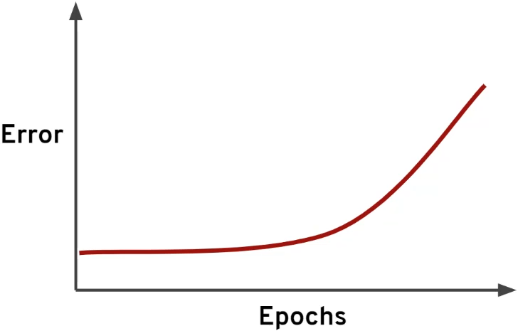
\includegraphics[width=0.5\textwidth]{fig/2-fundamentacao/overfitting/modelo_ruim.png}
                \fonte{\cite{Complete79:online}}
                \label{fig:modelo_ruim}
            \end{figure}
            
            Portanto, o estudo da simplicidade/complexidade dos modelos é importe para compreender a relação entre o desempenho deles nos conjuntos de treino e de teste/validação, sendo possível visualizar esse comportamento conforme as épocas passam. A Figura~\ref{fig:epocas_treino_teste} mostra os resultados ideais obtidos durante o treinamento, curva em vermelho, e de o teste, curva em azul.
            
            \begin{figure}[H]
                \centering
                \caption{Modelo ideal de erro de treino e de teste em relação ao as épocas.}
                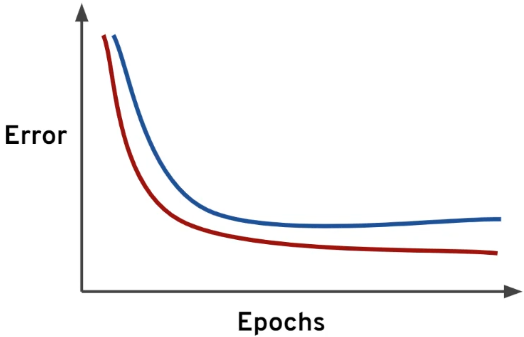
\includegraphics[width=0.5\textwidth]{fig/2-fundamentacao/overfitting/epocas_treino_teste.png}
                \fonte{\cite{Complete79:online}}
                \label{fig:epocas_treino_teste}
            \end{figure}
            
            No comportamento ideal, tanto o conjunto de treino como o de teste tem seu erro reduzido a medida em que as épocas passam. O resultado deles é similar, entretanto, no teste espera-se valores de perda maiores. Porém, se há sobre-ajuste, ao testa-los, tanto com os dados de teste como com os de validação, o resultado será ruim o que pode ser analisado na Figura~\ref{fig:Epoca_teste_ruim}.
            
            \begin{figure}[H]
                \centering
                \caption{Modelo ruim de erro de treino e de teste em relação ao as épocas.}
                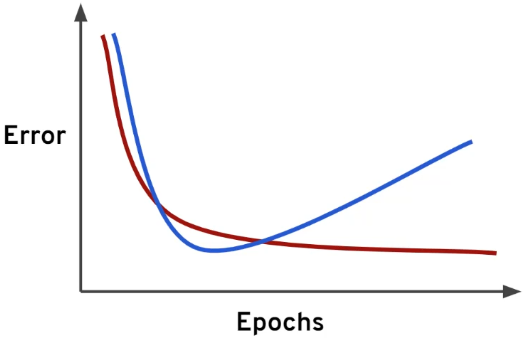
\includegraphics[width=0.5\textwidth]{fig/2-fundamentacao/overfitting/Epoca_teste_ruim.png}
                \fonte{\cite{Complete79:online}}
                \label{fig:Epoca_teste_ruim}
            \end{figure}
            
            O exemplo da Figura~\ref{fig:Epoca_teste_ruim} é uma boa indicação de complexidade excessiva nos dados de treino. Nela é possível visualizar o ponto no conjunto de teste, no qual o erro começa a aumentar ao invés de reduzir. Esse ponto define quando parar de treinar o modelo, pois, para as épocas a seguir começará o sobre-ajuste e os resultados para novos dados serão piores \cite{CollegeL30:online}. Esse ponto de corte é apresentado na Figura~\ref{fig:ponto_de_corte}.
            
            \begin{figure}[H]
                \centering
                \caption{Ponto de corte no tempo de treinamento para evitar sobre-ajuste.}
                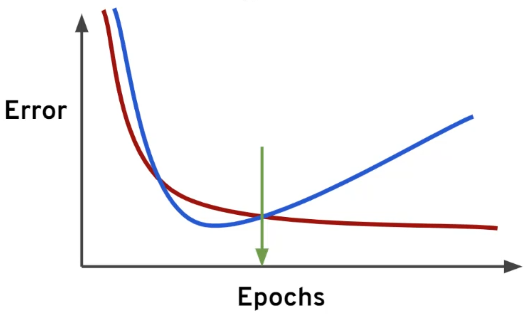
\includegraphics[width=0.5\textwidth]{fig/2-fundamentacao/overfitting/ponto_de_corte.png}
                \fonte{\cite{Complete79:online}}
                \label{fig:ponto_de_corte}
            \end{figure}
            
        \subsection{Avaliação de desempenho - Métricas de erro de classificação}\label{cap:metrica}
            
            Esta seção descreverá as métricas de avaliação de desempenho para problemas de classificação. Elas são utilizadas no final do processo de aprendizado, após o treinamento, com os dados do conjunto de teste e buscam avaliara eficiência do modelo. 
            
            As principais métricas de classificação estudadas por este trabalho são: acurácia, \textit{recall}, precisão e F1-Score. Antes de descrever-las, será explicado o raciocínio por trás delas e como realmente funcionam no mundo real. 
            
            Em uma típica tarefa de classificação, o modelo pode alcançar apenas dois resultados: ou ele realizou uma previsão correta; ou ele realizou uma previsão incorreta. Todas as métricas de classificação derivam dessa ideia, e felizmente, é possível expandi-la para situações em que há várias classes. Entretanto, para explicar o propósito delas será considerado uma classificação binária.
            
            A partir de um modelo que tem como objetivo classificar imagens como sendo de cachorro ou de gato, será descrito como determinar o desempenho real/final. O conjunto de teste possuí atributos, $x_{\text{test}}$, imagens de cachorro e gato, e seus respectivos rótulos, $y_{\text{test}}$, o nome cachorro e gato. 
            
            As imagens são dadas como entrada no modelo já treinado, que faz uma previsão. Esse resultado será uma predição correta, por exemplo, se a rede inferir cachorro para uma imagem de cachorro, como mostra a Figura~\ref{fig:cao_igual_cao}. 
            
            \begin{figure}[H]
                \centering
                \caption{Predição correta da rede neural.}
                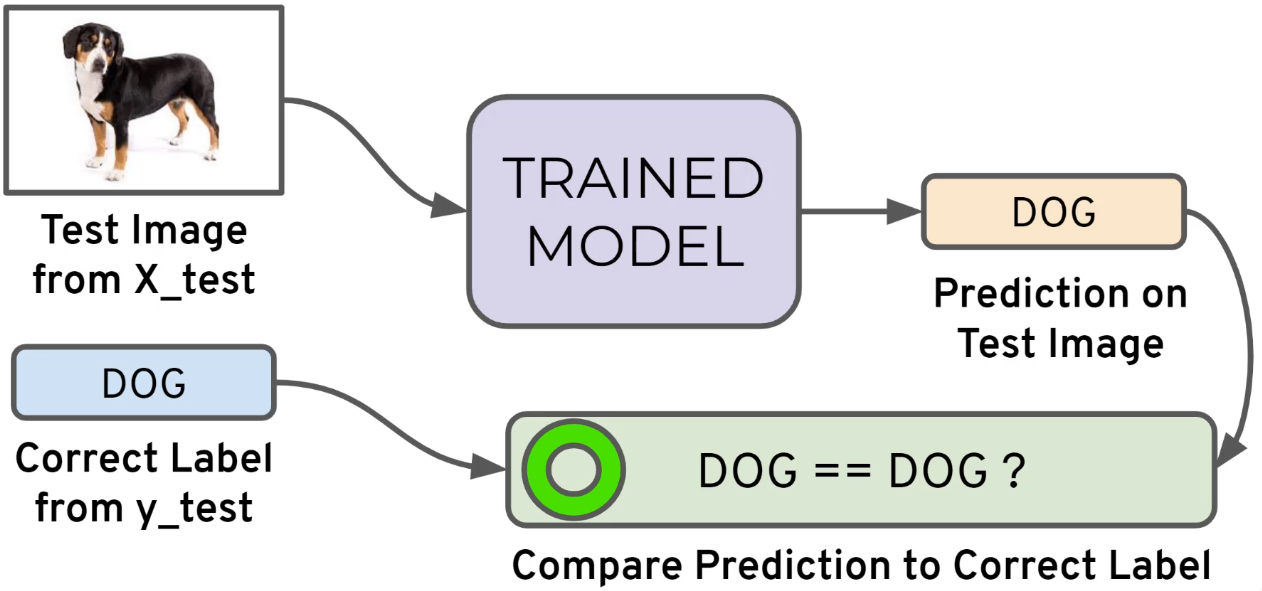
\includegraphics[width=0.5\textwidth]{fig/2-fundamentacao/metricas/cao_igual-cao.png}
                \fonte{\cite{Complete79:online}}
                \label{fig:cao_igual_cao}
            \end{figure}
            
            Porém, ela estará incorreta quando seu saída for gato e a imagem é de um cachorro, resultado apresentado pela Figura~\ref{fig:gato_nao_igual_cao}. 
        
            \begin{figure}[H]
                \centering
                \caption{Predição incorreta da rede neural.}
                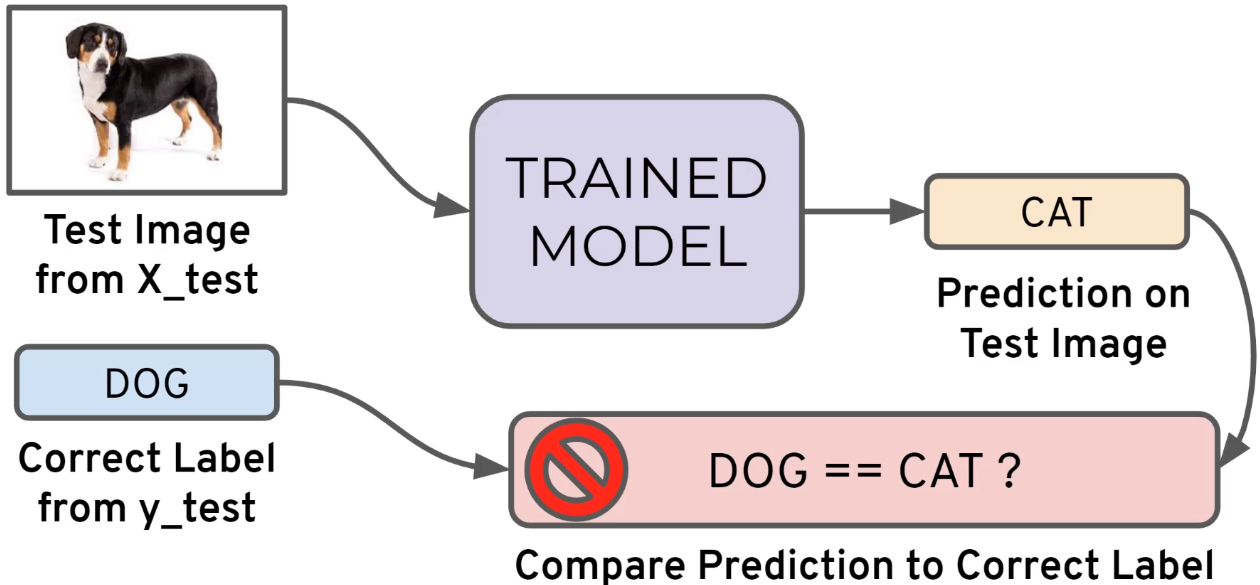
\includegraphics[width=0.5\textwidth]{fig/2-fundamentacao/metricas/gato_nao_igualcao.png}
                \fonte{\cite{Complete79:online}}
                \label{fig:gato_nao_igual_cao}
            \end{figure}
            
            Ao repetir esse processo para todas as imagens do banco de dados de teste, tem-se uma contagem das correspondências corretas e incorretas. É importante dizer que, no mundo real, nem todas as correspondências incorretas ou corretas têm o mesmo valor. Isso significa que uma única métrica não é o suficiente para caracterizar o desempenho do modelo. Portanto, são utilizados as quatro métricas e organiza-se os valores previstos em comparação com os reais no que é conhecido como matriz de confusão.
            
            A matriz de confusão apresenta os resultados de classificações corretas versus incorretas, como mostra a Figura~\ref{fig:matriz_confusão}. As condições verdadeiras (\textit{True Condition}) que indicam qual o rótulo correto/esperado para um dada inferência. Essas condições possuem duas subcategorias, positiva e negativa. Em outras palavras, é realmente cachorro versus não é, conforme Figura~\ref{fig:gato_nao_igual_cao}. As inferência realizadas pelo modelo são apontadas na condições de predição (\textit{Predicted Condition}), que também podem assumir duas categorias, positiva e negativa.
        
            \begin{figure}[H]
                \centering
                \caption{Matriz de confusão na qual computa predições em relação do que se esperava como \textit{output}.}
                \includegraphics[width=0.7\textwidth]{fig/2-fundamentacao/metricas/matriz_confusão.png}
                \fonte{\cite{Complete79:online}}
                \label{fig:matriz_confusão}
            \end{figure}
            
            Como é possível analisar, os elementos da diagonais da matriz apresentam as previsões corretas para diferentes classes, enquanto os dados fora da diagonal mostram as amostras que foram mal classificadas. Assim, as possibilidades de resultados de classificações são:
            \begin{itemize}
                \item Verdadeiro Positivo (\textit{True Positive} - TP): o modelo prediz corretamente a classe positiva;
                \item Verdadeiro Negativo (\textit{True Negative} - TN): o modelo prediz corretamente a classe negativa;
                \item Falso Positivo (\textit{False Positive} - FP): o modelo prediz incorretamente a classe positiva (erro tipo 1);
                \item Falso Negativo (\textit{False Negative} - FN): o modelo prediz incorretamente a classe negativa (erro tipo 2).
            \end{itemize}\\
            
            Considerando como classe positiva a imagem de cachorro e a negativa a de gato, tem-se os seguintes resultados:
            \begin{itemize}
                \item TP: é a imagem de um cachorro e o modelo predisse corretamente cachorro;
                \item TN: é a imagem de um gato e o modelo predisse corretamente gato;
                \item FP: é a imagem de um cachorro e o modelo predisse incorretamente gato;
                \item FN: é a imagem de um gato e o modelo predisse incorretamente cachorro;
            \end{itemize}
            
            A partir das informações discutidas até aqui, é possível compreender as métricas, começando pela acurácia, que pode ser calculada pela média dos valores situados na "diagonal principal". Neste caso, ela é escrita em termos de positivos e negativos como mostra a equação~\ref{eq:acuracia_positivo_negativo}.
            
            \begin{equation}
                \centering
                \text{Acurácia} = \frac{TP + TN}{TP + TN + FP + FN}
                \label{eq:acuracia_positivo_negativo}
            \end{equation}
            
            Frequentemente é definida como o número de previsões corretas feitas pelo modelo dividido pelo número total de predições, conforme a expressão~\ref{eq:acuracia}. Independente da forma escolhida para representa-la, a acurácia responde a pergunta, quantas predições corretas o modelo acertou em porcentagem. Por exemplo, um modelo terá uma acurácia de 80$\%$ se em um conjunto de testes com 100 imagens ele prever corretamente 80 delas. 
            
            \begin{equation}
                \label{eq:acuracia}
                \centering
                \text{Acurácia} = \frac{\text{Número de predições corretas}}{\text{Número total de predições}}
            \end{equation}
            
            O problema dessa métrica, é que ela é eficaz somente quando as classes alvo são bem balanceadas, isto é, sempre que há aproximadamente a mesma quantidade de imagens nas diferentes categorias. Mas em situações com desbalanceadas ela é péssima para determinar o desempenho. Para entender o significado disso, pode-se considerar um conjunto de teste com 99 imagens de cães e apenas uma de gato, e um modelo de uma linha que sempre irá prevê cachorro. A acurácia neste caso é de 99 $\%$, porque o único \textit{output} desta rede é cachorro, não importando a imagem dada a ela, e existem 99 imagens deles. Do contrário, se fosse uma reta constante na classe gato, o cálculo resultaria em 1 $\%$ de acurácia, pois existe somente uma imagem deste animal. O motivo de utilizar outras métricas é porque na maior parte das situações trabalha-se com desigualdade de rótulos.
            
            Entre as métricas utilizadas com classes desbalanceadas estão \textit{recall} e precisão. A primeira é definida como a capacidade de um modelo encontrar todos os casos relevantes dentro de um conjunto de dados, e sua definição precisa é dado pela equação~\ref{eq:recall}. Essa métrica tenta responder a pergunta: Qual proporção de positivos reais foi identificada corretamente? 
            
            \begin{equation}
                \centering
                Recall = \frac{TP}{TP + FN}
                \label{eq:recall}
            \end{equation}
            
            Já a precisão é a capacidade de um modelo de classificação identificar apenas os pontos de dados relevantes, sendo descrita matematicamente pela equação~\ref{eq:precisão}. O objetivo dela é responder a pergunta: Qual proporção de identificações positivas estava realmente correta?
            
            \begin{equation}
                \centering
                Recall = \frac{TP}{TP + FP}
                \label{eq:precisão}
            \end{equation}
            
            Constantemente, há a necessidade de encontrar o equilíbrio entre \textit{recall} e precisão. Para isso usa-se uma combinação delas que é conhecida como F1-Score. Ela é obtida através a média harmônica entre essas duas métricas, de acordo com a equação~\ref{eq:F1Score}. A F1-Score informa o quão preciso é o classificador, ou seja, quantas instâncias ele classifica corretamente, bem como, o quão robusto ele é, quer dizer, se ele não perde um número significativo de instâncias.
            
            \begin{equation}
                \centering
                F1-Score = 2\cdot\frac{\textit{precisão} \cdot recall}{\textit{precisão} + recall}
                \label{eq:F1Score}
            \end{equation}
            
            A razão para utilizar a média harmônica em vez da simples, é porque essa pune diferenças extremas. Por exemplo, se um classificador tem uma precisão igual à 1 (perfeita) e o \textit{recall} igual à zero (pior registro possível), com a média simples o resultado é igual a 0,5, já estimado com o F1-Score a solução é 0. Então, pode-se notar que F1-Score penaliza desproporções grandes de precisão e \textit{recall} e, portanto, é uma avaliação mais justa, principalmente para classes desbalanceadas. 
            
            A matriz de confusão e as várias métricas calculadas são maneiras de comparar o valor predito com o verdadeiro. Mas uma pergunta relevante é, qual dessas métricas é a "ideal"? A reposta depende da situação na qual o modelo está sendo executado, e do contexto do problema. Não existe um número único que possa afirmar o que é melhor. Por exemplo, não é possível declarar que $99\%$ de acurácia é bom o suficiente para todas as situações, já que para classes desbalanceadas isso não se aplica. A mesma observação vale para precisão e \textit{recall}, pois, ao ajustar o resultado para diminuir um, o outro será aumentado. Ou seja, é necessário decidir se o modelo deve se concentrar na correção de falsos positivos ou nos de falsos negativos. Essa constatação pode ser exemplificada ao substituir o exemplo da classificação de imagens por a de diagnóstico de doença. 
            
            No problema de predição de doenças, dificilmente haverá uma enfermidade que cerca de metade da população seja afetada e a outra não, logo, é um problema de classes desbalanceadas. Isso causa um "cobertor curto" entre precisão, que diminuindo melhora os FP, e \textit{recall}, que diminuindo melhora os FN. É importante ressaltar que, modelos de inteligência artificial, em situações de problemas de saúde são usados como diagnóstico rápido antes de realizar um exame mais invasivo, pois, na investigação de patologias mais severas, as "apostas" são altas. Neste caso, é melhor tentar minimizar o número de falsos negativos ao custo de aumentar o de falsos positivos. para se ter certeza de que foram classificados corretamente o maior quantidade possível de casos. 
            
            Portanto, o ideal nesta cenário é que todas as pessoas doentes passem para a próxima etapa, isso é muito importante, pois os modelos de inteligência artificial não são perfeitos. Dessa forma, é melhor diagnosticar uma pessoa como enfermar e garantir que ela siga sendo acompanhada para no futuro, com outros exames, possa ser dispensada como um diagnóstico errado, do que não tratar uma pessoa enferma. Isso considerando que haverão testes complementares, que por mais invasivos possam confirmaram ou não esse resultado prévio. O oposto é verificado na fabricação de equipamento, onde prefere-se que máquinas sem defeito sejam descartadas (FP) do que as com mau funcionamento sejam entregues ao consumidor final (FN).
            
            Existem outras métricas calculáveis que tentam prever o desempenho de modelos, entretanto, este trabalho irá abordar somente as descritas neste capítulo. Para mais informação sobre outras possibilidade de determinar a performance podem ser estudadas em\todo{citar bibliografia wikipédia}. 
        
            
        \subsection{Regressão logística para classificação binária}
        
            Muitos problemas requerem uma estimativa de probabilidade como saída. A regressão logística é um mecanismo extremamente eficiente para o cálculo de probabilidades. Em termos práticos, pode-se usar o resultado da probabilidade de uma das seguintes maneiras: como é; ou convertido em uma categoria binária.
            
            Usando sem alteração, "como está", é calculado pela probabilidade de $A$ ocorrer dado $B$, definido por~\ref{eq:probabilidade_A|B}.
            
            \begin{equation}
                \centering
                p(A|B)
                \label{eq:probabilidade_A|B} 
            \end{equation}
            
            É possível converter o resultado da probabilidade para um valor binário, ou seja, para uma classificação (tema deste trabalho). Isso é realizado a partir de um limiar, também conhecido por limite de decisão, que define quando um valor de probabilidade passa de uma categoria para outra.
            
            Para garantir que a saída do modelo de regressão logística fique entre 0 e 1, é usado uma função sigmoide, que produz o seguinte gráfico, apresentado na Figura~\ref{fig:sigmoide}. 
        
            \begin{figure}[H]
                \centering
                \caption{Função sigmoide.}
                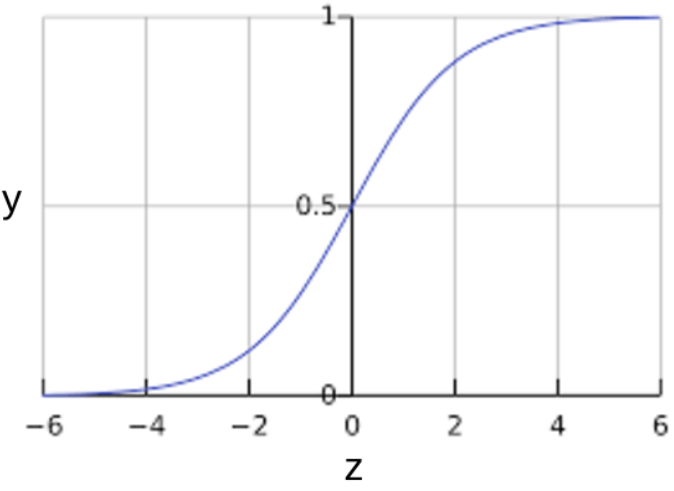
\includegraphics[width=0.5\textwidth]{fig/2-fundamentacao/aprendizado/sigmoide.png}
                \fonte{\cite{MachineL6:online}}
                \label{fig:sigmoide}
            \end{figure}
            
            Se $z$ representa a saída da camada linear de um modelo treinado com regressão logística, então sigmoide ($z$) produzirá um valor (uma probabilidade) entre 0 e 1, dado pela equação~\ref{eq:sigmoide}. 
            
            \begin{equation}
                \label{eq:sigmoide}
                \centering
                y = \frac{1}{1 + \exp^{-z}}
            \end{equation}
            
            em que:
            \begin{itemize}
                \item $y'$ é a saída do modelo de regressão logística para um exemplo específico;
                \item $z = b + w_{1}x_{1} + w_{2}x_{2} + ... + w_{N}x_{N}$
                \begin{itemize}
                    \item $w$ são os pesos aprendidos pelo modelo;
                    \item $b$ é o bias aprendido pelo modelo;
                    \item $x$ são as atributos para um exemplo específico.
                \end{itemize}
            \end{itemize}
            
            $Z$ também é conhecido como \textit{log-odds} porque o inverso da sigmoide, dado pela equação~\ref{eq:log_odds}. Ele afirma que, $z$ pode ser definido como o \textit{log} da probabilidade de "1"\textit{ }rótulo dividido pela probabilidade do "0"\textit{ }rótulo.
            
            \begin{equation}
                \centering
                z = \log\left(\frac{y}{1 - y}\right)
                \label{eq:log_odds}
            \end{equation}
            
            Para exemplificar, considere um modelo de regressão logística que recebera como paramenteiros de entrada os seguintes valores e atributos:
            
            \begin{itemize}
                \item bias: $b = 1$;
                \item peso 1, 2 e 3: $w_{1}$, $w_{2}$ e $w_{3}$;
                \item atributos 1, 2 e 3: 0, 10 e 2.
            \end{itemize}
            
            $z$ é dado pelo desenvolvimento a segui:
            \begin{equation*}
                z = b + w_{1}x_{1} + w_{2}x_{2} + w_{3}x_{3}
            \end{equation*}
            
            \begin{equation*}
                z = 1 + 2\cdot0 + (-1)\cdot10 + 5\cdot2
            \end{equation*}
            
            \begin{equation*}
                z = 1
            \end{equation*}
            
            Substituindo $z = 1$ na equação~\ref{eq:sigmoide}, obtém-se o seguinte resultado demonstrado pela Figura~\ref{fig:probabilidade_output}: 
            
            \begin{equation*} 
                \centering
                y = \frac{1}{1 + \exp^{-1}}
            \end{equation*}
            
            \begin{equation*} 
                y = 0,731
            \end{equation*}
        
            \begin{figure}[H]
                \centering
                \caption{Saída da regressão logística.}
                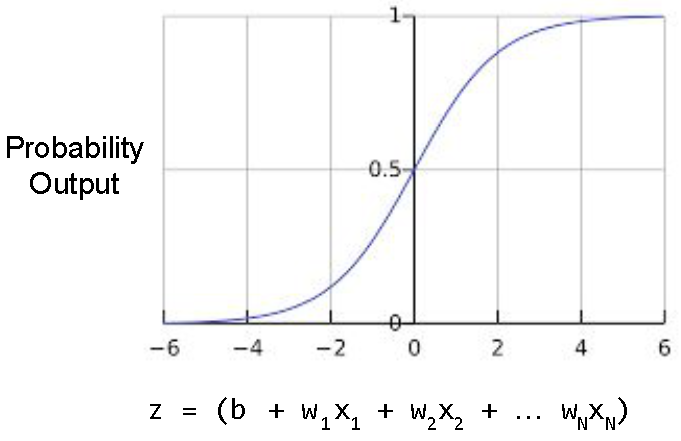
\includegraphics[width=0.5\textwidth]{fig/2-fundamentacao/aprendizado/probabilidade_output.png}
                \fonte{\cite{MachineL6:online}}
                \label{fig:probabilidade_output}
            \end{figure}
% ----------------------------------------------------------
\chapter{Metodologia}


\chapter{Resultados e discussão}
% ----------------------------------------------------------
\chapter{Conclusões}
% --------------------------------------------------------

% ----------------------------------------------------------
\chapter{Rascunho}
% --------------------------------------------------------

% \section{Introdução}


%     % Para desenvolver produtos, equipamentos, salas, etc, com características  acústicas adequadas é necessário entender as propriedades da fonte sonora, do meio meio de propagação, assim como compreender a forma como o cérebro humano codifica e decodifica fenômenos sonoros. Dessa forma, é importante realizar inicialmente  uma correta identificação dos sinais como um primeiro passo na criação e aperfeiçoamento desses dispositivos (aparatos) ou na detecção de problemas.
    
%     Os padrões sonoros permitem identificar características importantes do comportamento de sistemas dinâmicos possibilitando ao ser humano identificar os mais variados fenômenos. Com as habilidades auditivas e vocais, um individuo é capaz de gerar e discernir barulhos sem significados, fonemas, palavra, frases, até, em uma conversar conseguir encontrar o local de origem de um locutor pelo seu sotaque e regionalismos. Também é possível criar sons com ritmos, timbres, estilos diferentes assimilando assim sues contrastes. Essa capacidade é vista até para dar significado a alertas sonoros, barulhos causados por animais, ruídos, batidas, entre outros. 
    
%     As aptidões humanas de classificação foram relevantes no seu desenvolvimento e na forma de interagir com o mundo. Logo, as descrição de comportamento de sistemas foram e são estudadas para desenvolver técnicas que possibilitam aperfeiçoar e, ou adicionar recursos em produtos e serviços. Como também orientar a criação de ferramentas e a detecção de problemas. A identificação de falhas ou condições atípicas de operação em máquinas é uma aplicação interessante, pois pode ser verificada diariamente nos produtos. Por exemplo, ao girar o volante de uma carro todo para um lado gerar um som tipico de homocinética, o condutor pode considerar esta ocorrência como um alerta de problema. Neste caso, ele é capaz de pensar em algum defeito no eixo do carro, ou se não tem conhecimento para tal, levar o automóvel a uma mecânica para conserto. Isso remete que, alguns sinais relatam tanto a visos de avaria como também a qualidade do dispositivo.
    
%     % Uma aplicação interessante é a detecção de falhas ou condições atípicas de operação em máquinas, que pode ser verificada diariamente nos produtos. Por exemplo, se ao girar o volante de uma carro todo para um lado gera um som de "clap, clap" tipico de homocinética, ele é considerado um alerta de problema, o qual, pode remeter ao condutor que o eixo do carro possuí um defeito. Esses sinais sonoros são avisos para o consumidor, como também uma característica que descreve sua qualidade.

%     No contexto industrial, as orientações de conserto são aplicáveis em série, assim como as de reconhecimento de mau funcionamento nas linhas de produção. Essas ferramentas são automatizadas para a fabricação de equipamento em baixo custos e otimizada, portanto, outra prática relevante é o monitoramento a partir de sistemas embarcados, que é vantajoso em situações de grande prejuízo caso a falha no equipamento não seja detectada imediatamente. Nestes casos, o interessante é obter uma análise prévia, se não imediata do problema, para uma abordagem simples e efetiva, gerando menos perdas de material e tempo.

%     % No contexto industrial é possível orientar o conserto ou fabricação de equipamento, reduzir custos e otimizar sistemas para o reconhecimento de mau funcionamento tanto em linhas de produção como em reparo. Também é possível realizar monitoramento a partir de sistemas embarcados, o que é vantajoso em situações de grande prejuízo caso a falha no equipamento não seja detectada imediatamente. Nestes casos, o interessante é obter uma análise prévia, se não imediata do problema, para uma abordagem simples e efetiva, gerando menos perdas de material e tempo.
    
%     Do ponto de vista técnico a classificação consiste em extrair características tanto físicas quanto perceptivas de um sinal sonoro e, a partir disso, definir uma classe na qual o evento em questão melhor se enquadra. Para isso, pode-se utilizar algoritmos de extração e classificação de recursos que são bastante diversificados. Uma forma de simplificar essa escolha é ter em mente que ela depende do domínio no qual a análise será realizada. 
    
%     Atualmente, novos métodos estão sendo estudados, entre eles a classificação automática de sinais sonoros utilizando IA. Essa é uma área crescente de pesquisa com inúmeras aplicações no mundo real existindo uma grande quantidade de trabalhos em campos relacionados ao áudio, como fala e música, e alguns trabalhos sobre a classificação de sons ambientais. O conteúdo desses estudos são empregados em produtos e serviços tais como: aplicativos de reconhecimento de fala ou musica, assistente residenciais, próteses auditivas, sistemas de automatização, carros, entre outros. 
    
%     É importante averiguar essas tecnologias emergentes tanto no sentido de inovação de produtos quanto na análise preditiva para detecção de prováveis avarias de amostras. Uma aplicação que ainda carece de estudos aprofundados é a classificação de padrões sonoros de compressores hermético utilizando algoritmos de inteligência artificial.
    
%     O compressor é um dos responsável pela circulação de fluído ao longo do sistema de refrigeração, junto com o condensador, válvula de expansão e evaporador torna possível o ciclo de refrigeração. Ele também é uma das fonte sonoras mais importantes desse conjunto, as energias vibratórias produzidas no seu interior são transmitidas dele ao ambiente com níveis de ruído consideráveis. Dessa forma, identificar os ruídos anômalos dos típicos é de suma importância para indicar falas de operação ou descrever a qualidade sonora do produto final.
    
%     % O compressor é um dos principais dispositivos no processo de refrigeração, ele possuí ruídos típicos e anomolos. Os anomolos podem indicar falhas de operação ou qualidade sonora.
%     % causo por forças magnéticas geradas nos espaços existentes entre o rotor e o estator. 
    
%     Portanto, de todos os sinais radiados por compressores herméticos, foram escolhidos alguns padrões para treinar redes neurais à classifica-los. Essa será uma primeira análise para que em trabalho futuros seja possível reconhecer anomalias no sistema. Entre os sons escolhidos estão: \textit{dripping}, \textit{knock}, \textit{start stop}, \textit{molas}, operação estacionária.\\
    
%     NO FINAL DO TRABALHO VOLTAR PARA DESCREVER TODOS OS SINAIS ESCOLHIDOS.

%     \todo{apresentar trabalhos na área de classificação fala, musica e sons ambienta}

%     \todo{apresentar trabalhos na área de classificação industrial}

%     \todo{apresentar trabalhos sobre compressores}

%     \todo{apresentar trabalhos sobre compressores}


%     \section{Objetivos}    

%         \todo{Escrever objetivos no final do trabalho quando todo os esboço for terminado}
        
%         A partir do exposto anteriormente e da necessidade de identificar padrões sonoros de como pressores, como \textit{dripping}, \textit{knock}, \textit{start} \textit{stop}, batida de mola. O objetivo deste trabalho é determinar a eficácia diferentes algoritmos de inteligência artificial para reconhecer e classificar padrões de falhas a partir de sinais pressão e vibração produzidos por compressores herméticos de sistemas de refrigeração.
%         %da rede neural recorrente chamada de Memória de Longo Prazo (LSTM\footnote{Acrônimo do inglês para \textit{Long Short Term Memory.}}) para reconhecer e classificar padrões de sinais sonoros produzidos por compressores herméticos de sistemas de refrigeração.
    
%     \subsection{Objetivos específicos}
    
%         \begin{itemize}
%             \item Investigar o funcionamento de diferentes algoritmos de redes neurais para detecção de padrões em sinais de sistemas de refrigeração;
%             \item Implementar rotinas de treinamento e classificação de maneira organizada e intuitiva para utilização posterior do LVA e empresas parceiras;
%             \item Investigar o comportamento dos algoritmos com diferentes tipos de entradas, tais como sinais de pressão sonora e aceleração.
%         \end{itemize}

%     \subsection{Organização do trabalho}
        
%         A estrutura de trabalho está organizada da seguinte forma, há (TANTOS) capítulos. O primeiro é uma introdução dos trabalho de padrão sonoros, das áreas que são beneficiadas por estas técnicas e do motivo de utilizar algoritmos de inteligência artificial para classificar em classes sinais sonoros de compressores.
    
%         No Capítulo 2 é apresentado o referencial teórico, no qual são descritas as principais teorias utilizadas para o trabalho, tendo como base  a literatura e as normas referentes a cada área necessária para o desenvolvimento do trabalho.\\
        
%         QUANDO TERMINAR OS OUTROS CAPÍTULOS ESCREVER O RESTO
    
%%%%

% \section{Diferença entre \ai, \ml e \dl}

%     Os temas \ai, \ml e \dl são discutidos assiduamente nos meios de comunicação, em estudos, sendo vendidos como diferencias de produtos. Portanto nesta seção será definido cada uma dessas áreas ou subáreas, apresentando suas diferenças.

%     A \ai, \todo{cite DeepLearningArtigo} se propõe elaborar dispositivos que simulem a capacidade humana de raciocinar, perceber, tomar decisões e resolver problemas. Logo, qualquer técnica que permita computadores imitar o comportamento humano pode ser definido com um IA. 

%     \ml \todo{cite DeepLearningArtigo} é um subárea de IA. Seu intuito é fazer que as máquinas aprendam sozinhas usando dados fornecidos e assim, consigam realizar previsões com uma dada incerteza. Dentre os algorítimos de ML existe um outro subconjunto conhecido como \dl focado em redes neurais (NN \footnote{Acrônimo do inglês para \nn.}).  
    
%     As \nn são uma forma de modelar matematicamente sistemas neurônios biológicos, e utiliza-los para resolver tarefas que outros tipos de algoritmos não conseguem realizar, ex.: classificação de imagens. Os subconjuntos de que compõem a IA podem ser visualizados na Figura \todo{ref fig: AI Ml DL}.
    
%     A ideia de \dl ser um "tipo" de \ml é muito importante, e este é o motivo de realizar uma revisão sobre como IA, ML e DL estão relacionados. O \dl por ter resolvido com proficiência alguns problemas que desafiaram a \ai esta em destaque recentemente. Seu desempenho é excepcional em muitos campos, no entanto, também enfrenta limitações. Essas limitações derivam de seus conceitos fundamentais os quais foram herdados de seu ancestral, o ML. Como uma subárea do aprendizado de máquina, o aprendizado profundo não pode evitar os problemas base que o ML enfrenta. Por isso que precisa-se apresentar o \ml antes de discutir o conceito de \dl, o que será feito na seção~\ref{cap:ML}, porque um é alicerce do outro. 
    
%     % \begin{figure}[H]
%     %     \centering
%     %     \includegraphics[width=0.8\textwidth]{fig/RefBiblio/Areas.png}
%     %     \caption{Esquemático dos subconjuntos da AI. Fonte: adaptado de \cite{RevolucaoIA}.}
%     %     \label{fig:ALMLDL}
%     % \end{figure}
    
%     % A diferença principal diferença entre ML e DL, é que este último é composto de várias camadas de redes neurais, também conhecido como \textit{Layers}, como mostra a Figura~\ref{fig:MlDl}. Quanto maior o número de camadas, mais profundo o modelo.
    
%     % \begin{figure}[H]
%     %     \centering
%     %     \includegraphics[width=0.8\textwidth]{fig/RefBiblio/MLDL.png}
%     %     \caption{Diferença entre ML, \textit{simple neural network}, e DL, \textit{deep learning neural network}. Fonte: \cite{NotesAiMlDl}.}
%     %     \label{fig:MlDl}
%     % \end{figure}
    
%     % No DL, cada \textit{Layer} recebe uma entrada da camada anterior e a passa para a próxima. Dessa forma, as primeiras lidam com recursos mais genéricos e mais grosseiros e, na medida que a rede se aprofunda, ela consegue aprender detalhes mais precisos do conjunto de dados. No final, fornece uma saída com um certo fator de confiança. Esse procedimento ameniza um dos problemas mais difíceis 
%     % do ML: a engenharia de recursos. 
    
%     % A engenharia de recursos lida com a extração de recursos adequados que podem ser inseridos no modelo e assim, determinar se o modelo será defeituoso, ou seja, com alta variância. Para isso, deve-se ter cuidado para que os recursos não estejam incompletos ou em grande número, sendo que nem todos contribuírem para a previsão do modelo. Ou seja, o algoritmo não pode apresentar falhas de alto viés. Portanto se houver muitos recursos, é necessário um conjunto de dados muito grande para aprender, caso contrário, o modelo é falho. 
    
%     % \begin{figure}[H]
%     %     \centering
%     %     \includegraphics[width=0.8\textwidth]{fig/RefBiblio/DadosEntrada.png}
%     %     \caption{Diferença na extração das características nos algoritmos de ML e DL. Fonte: \cite{NotesAiMlDl}.}
%     %     \label{fig:DadosEntrada}
%     % \end{figure}
    
%     % Os recursos nos sinais da camada de entrada são aplicados a partir de uma representação digitalizada, por exemplo, uma imagem, som, áudio, etc. A extração de recurso desses sinais é realizado de forma automática com os algoritmos de DL. Isso significa que eles automaticamente captam as características relevantes necessárias para a solução do problema e realizam este processo minimizando os erros (viés nos dados). Na Figura~\ref{fig:DadosEntrada} é ilustrada a diferença da engenharia de recursos dos algoritmos de ML e DL. 
    
%     % Portando, as redes neurais de DL, nas aplicações que não exigem uma intervenção direta do ser humano, conseguem obter uma reposta com um menor viés. No caso da classificação de padrões em sinais sonoro, existem muitas arquiteturas de redes neurais usadas no processamento de áudio. As principais incluem redes totalmente conectadas, que são uma base para vários auto-codificadores. Como por exemplo, as redes neurais convolucionais  (CNN\footnote{Acrônimo do inglês para \textit{Convolutional Neural Network.}}), que distinguem atributos de fluxos de áudio e redes neurais recorrentes (RNN\footnote{Acrônimo do inglês para \textit{Recurrent Neural Network.}}), que são bem adaptadas para o processamento de diferentes sequências de tempo. Essas serão descritas na seções~\ref{Sec:RevConv} e \ref{Sec:RevRNRLSTM}  respectivamente.

%     % COLOCAR AQUI A DIFERENÇA ENTRA AI, ML E DL

%     % EXPLICAR QUE DL É UM TIPO DE ML E COMO TAL TEM OS MESMO PROBLEMS, PORTANTO ENTENDER ML É UM PASSO PARA COMPREENDER DL. PORTANTO, PRIMEIRO SERÁ EXPLICADO MACHINE LEARNING E EM SEGUIDA DL E AS REDES NEURAIS UTILIZADAS NESTE TRABALHO

% \section{Machine Learning}\label{cap:ML}

%     % OLHAR ESTE PARÁGRAFO
    
%     Uma outra forma de compreender as técnicas de \ml, é entende-lo como método de análise de dados que visa automatizar a construção de modelos analíticos. Seus algoritmos são capazes de aprender iterativamente com os dados, possibilitando que computadores encontrem \textit{insights} sem serem explicitamente programados sobre onde e o que procurar nas informações.
    
%     Posto isso, nesta seção serão apresentadas as terminologias básicas necessárias em \ml, como se dá o aprendizado e de que formar seus erros são reduzidos. Também será discutida a diferença entre tarefas \textit{supervised} e \textit{unsupervised}, assim como a distinção entre classificação e regressão. No final, serão descritas as métricas de avaliação de performance de modelos de classificação.
    
%     \subsection{Terminologias Fundamentais de ML e Introdução a Conceitos Básicos}

%         % Nesta subseção serão definidas terminologias fundamentais de \ml, e consequentemente de \dl, A partir disso, é possível determinar conceitos como: tipos de tarefas em ML, diferenças entre treinamento e inferência do modelo e entre classificação e regressão, e assim por diante.
        
%         % , como: \textit{labels}, \textit{features}, \textit{label} e \textit{unlabel} \textit{examples}, entre outros

%         Nesta subseção serão definidas terminologias fundamentais de \ml, e consequentemente de \dl, A partir disso, é possível determinar conceitos como: tipos de tarefas, diferenças entre treinamento e inferência e assim por diante.

%         Há dois tipos de tarefas em \ml, as \textit{supervised} (supervisionadas) e as \textit{unsupervised} (não supervisionadas). A \textit{supervised} aprende como a combinar inputs para produzir previsões úteis sobre dados nunca antes vistos, ou seja, se tem conhecimento sobre qual é a saída para uma dada entrada. Já no caso de não ter noção prévia do que espera-se como inferência das redes, utiliza-se modelos \textit{unsupervised}.
    
%         Duas terminologias muito importantes em \ml \textit{supervised}, que são os \textit{labels} (rótulos) e as \textit{features} (características/recursos). Os \textit{labels}, são as classes e também o que se espera como predição do modelo, representado pela variável $y$. As \textit{features}, são as variáveis de entrada
%         (valores que caracterizam as amostras), determinado por $x$. 
        
%         Uma das formas de indicar o quão sofisticado é um projeto de aprendizado de máquinas é através da quantidade de \textit{features}. Ou seja, redes que recebem como inputs poucos recursos são mais simples que as com múltiplas entradas. 
        
%         Do conjunto de amostras, um \textit{examples} é uma instância particular de dados do vetor de \textit{features} $\mathbf{\overline{x}}$ e são classificados em duas categorias: \textit{labeled examples} e \textit{unlabeled examples}. 
        
%         Um \textit{labeled examples} incluí tanto \textit{feature(s)} como o \textit{label(s)}. Ou seja:
%         \begin{center}
%             labeled examples: \{features, label\}: (x, y)
%         \end{center}

%         Já um \textit{unlabeled example} contem apenas as \textit{feature(s)} sem o \textit{label}. Como representado a seguir:
%         \begin{center}
%             labeled examples: \{features, ?\}: (x, ?)
%         \end{center}

%         Os problemas mais comuns resolvidos com este tipo de ML são os de regressão e classificação. Uma diferença entre eles, é que a regressão predizer valores contínuos, enquanto a classificação valores discretos. Outra mudança importante ocorre na forma de avaliar performance, com métricas específicas para cada um. Elas serão descritas na seção~\ref{cap:metrica}. 
        
%         De tudo o que foi exposto até agora, é possível concluir que modelos de classificação e regressão necessitam de um banco de dados prévio, visto que utilizam \textit{labeled} e \textit{unlabeled examples}, ou seja, são tarefas \textit{supervised}. Já no caso de \textit{unsupervised learning}, que não sabe-se o \textit{output}, exemplos comuns de aplicação são: problemas como detecção de anomalias (não se tem conhecimento do problema); \textit{cluster} (agrupamentos individuais); e redução de dimensionalidade\todo{citar trabalhos sobre cada um}. Como este trabalho será sobre classificação de padrões sonoros, as técnicas de \textit{unsupervised learning} não serão abordadas.

%         % Agora, quando não há um histórico de dados no qual é de conhecimento prévio o \textit{output} esperado, trabalha-se com \textit{unsupervised} \ml. Que resolve 

%         Para finalizar as definições básicas, necessita-se determinar o que é modelo, isso do ponto de vista de tarefas supervisionadas. Ele tem duas fases, que são:

%         \begin{itemize}
%             \item \textit{Training}: fase na qual o modelo aprende, ou seja, ele receberá \textit{labeled examples} e será permitido que ele gradualmente encontre a relação entre $x$ e $y$;
%             \item \textit{Inference}: momento que será aplicado o modelo treinado em \textit{unlabeled examples}, isto é, ele faz predições uteis ($y'$).
%         \end{itemize}


%     \subsection{Treinando modelo simples para compreender \ml}
        
%         A Figura~\ref{fig:dados_quaisquer} apresenta uma pequena amostra de dados observados, e a partir delas deseja-se encontrar uma relação entre $y$, variável de interesse dependente que se quer predizer, e $x$ a variável independente.
        
%         \begin{figure}[H]
%             \centering
%             \caption{Pequena amostra de dados quaisquer.}
%             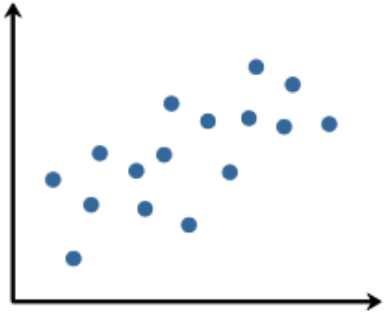
\includegraphics[width=5cm]{fig/2-fundamentacao/treinar_modelo_simples/dados_quaisquer.png}
%             \fonte{}
%             \label{fig:dados_quaisquer}
%         \end{figure}
        
%         Pela análise da Figura~\ref{fig:dados_quaisquer} é possível dizer que, uma reta consegue inferir o comportamento entre $x$ e $y$, mesmo que não passe exatamente por todos os pontos, como a Figura~\ref{fig:dados_quaisquer_regressao} demonstra. Matematicamente é descrita pela equação~\ref{eq:reta} na convenção estabelecida em ML e adicionando o subíndice que indica a possibilidade de ter mais de uma dimensão. Para inferir $y$, basta substituir os valores de $x$ neste modelo (reta).
        
%         \begin{equation}\label{eq:reta}
%             \centering
%             y' = b + w_{1}x_{1}
%         \end{equation}
    
%         \begin{enumerate}
%             \item[] em que:
%             \begin{itemize}
%                 \item $y'$ é o \textit{predicted label} (\textit{output} desejado);
%                 \item $b$ é o bias (intercepção no eixo $y$);
%                 \item $w_{1}$ é o peso da \textit{feature} 1. Peso tem o mesmo conceito que a inclinação ($m$) tem na equação tradicional da reta;
%                 \item $x$ é a \textit{feature} (\textit{input}).
%             \end{itemize}
%         \end{enumerate}

%         \begin{figure}[H]
%             \centering
%             \caption{Regressão linear que prever o comportamento da pequena amostra de dados quaisquer.}
%             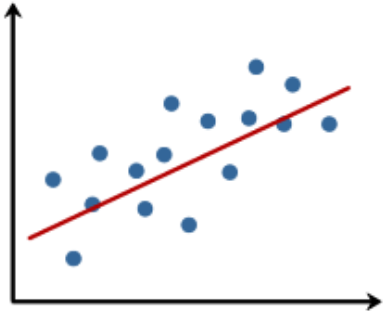
\includegraphics[width=5cm]{fig/2-fundamentacao/treinar_modelo_simples/dados_quaisquer_regrassao.png}
%             \fonte{}
%             \label{fig:dados_quaisquer_regressao}
%         \end{figure}
        
%         O exemplo proposto considerar somente uma dimensão de \textit{feature} como entrada, ao contrário de modelo mais sofisticado que utilizam muito mais, e com isso, possuem mais pesos ($w$). Logo, há um peso para cada \textit{feature} separado, como descreve a equação~\ref{eq:reta_varias_features}.
        
%         \begin{equation}
%             \centering
%             y' =  b + w_{1}x_{1} + w_{2}x_{2} + ... + w_{n}x_{n}
%             \label{eq:reta_varias_features}
%         \end{equation}
        
%         Para sintetizar, os dados foram aplicados em um algoritmo de \ml e como resultado obteve-se um modelo, que neste caso é uma reta. Mas é gerado uma a pergunta: como o treinamento realmente acontece? Ele ocorre ao determinar bons valores para o bias e todos os pesos utilizando \textit{labeled examples}. Para isso, o algoritmo examina varias amostras, e compara a predição feita pela equação criada, com o valor real, tentando encontrar um modelo que minimize a perda entre $y$ e $y'$.
        
%         A perda é também conhecida como erro, que dado por um número o qual indica o quão mal foi a inferência de um exemplo único. Ele pode ser visto como uma penalidade dada ao modelo por fazer uma predição ruim. Se $y'$ for igual a $y$, a perda será zero, caso contrário, será muito maior. 
        
%         A Figura~\ref{fig:loss_learning} apresenta dois modelos, sendo que o da esquerda possui um erro alto. Uma forma de concluir isso, é através da distância muito maior entre a linha azul (equação) e o ponto (valor verdadeiro). Enquanto, o gráfico da direta esse espaço é pequeno, mostrando que a perda é menor.

%         \begin{figure}[H]
%             \centering
%             \caption{Alta perda no modelo da esquerda e baixa perda no modelo da direita.}
%             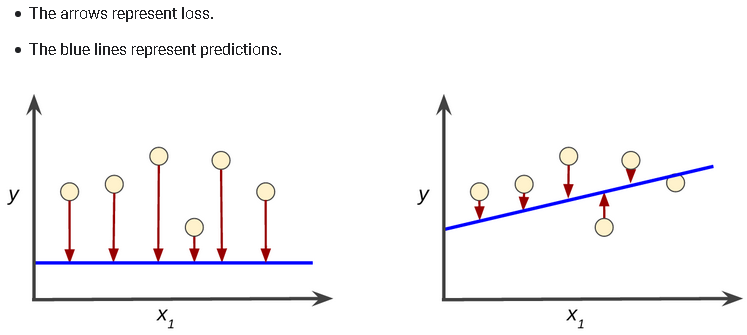
\includegraphics[width=0.7\textwidth]{fig/2-fundamentacao/aprendizado/loss_learning.png}
%             \fonte{}
%             \label{fig:loss_learning}
%         \end{figure}
        
%          Portanto o objetivo dos algoritmos de ML e DL, é treinar o modelo para encontrar os valores de $w_i$ e $b$ que minimize essa diferença ao longo de todos os exemplos. A equação mais comum usada para esse cálculo é \textit{squared loss} (erro quadrático), entretanto, ela é usada a partir do valor médio, denominado \textit{Mean square Error} (MSE, erro médio quadrático) e descrito pela equação~\ref{fig:MSE}.
        
%         \begin{equation}
%             \centering
%             MSE =  \frac{1}{N} \sum_{(x,y)\in D}  (y - y')^2
%             \label{eq:MSE}
%         \end{equation}
    
%         \begin{enumerate}\label{fig:MSE}
%             \item[] em que:
%             \begin{itemize}
%                 \item $(x,y)$ é um exemplo no qual
%                 \begin{itemize}
%                     \item $x$ é o conjunto de \textit{features} que o modelo usa para realizar predições;
%                     \item $y$ é o rótulo do exemplo.
%                 \end{itemize}
%                 \item $y'$ é a função de pesos e bias em combinação com o conjunto de \textit{features} $x$;
%                 \item $D$ é um conjunto de dados contendo muitos \textit{labels examples}, nos quais $(x,y)$ são pares;
%                 \item $N$ é o número de exemplos em $D$.
%             \end{itemize}
%         \end{enumerate}
        
%   \subsection{Redução de Perda}     

%         O diagrama apresentado na Figura~\ref{fig:abordagem_iterativa}, demonstra como o modelo de aprendizado de máquina reduz a perda iterativamente para aprender. Esse processo começa com o algoritmo gerando um "palpite", ou seja, um valor para $b$ e $w_1$. Então, o erro é calculado através da equação~\ref{eq:MSE}. 
        
%         As entradas, na estimativa da perda, são o conjunto de \textit{label}, $y$, e a inferência, $y'$, realizada pelo primeiro modelo utilizando o conjunto de \textit{features}. Após é repetido este processo, entretanto com um novo palpite e da comparação entre os resultado obtidos, o algoritmo escolhe qual das tentativa obteve o menor erro.

%         \begin{figure}[H]
%             \centering
%             \caption{Abordagem iterativa para o treinamento do modelo através da redução do erro.}
%             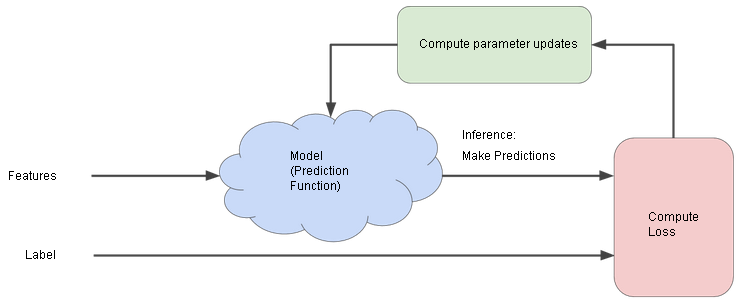
\includegraphics[width=0.8\textwidth]{fig/2-fundamentacao/aprendizado/abordagem_iterativa.png}
%             \fonte{}
%             \label{fig:abordagem_iterativa}
%         \end{figure}
        
%         O diagrama~\ref{fig:abordagem_iterativa} tem uma etapa chamada de \textit{Compute Loss}, que representa o momento no qual o algoritmo determina o erro. Na sequência, há o processo \textit{Compute Parameter Updates}, que caracteriza a rede examina os valores calculados pela função de perda e escolher como será a atualização deles. Esse procedimento de aprendizado continua a cada iteração até que o algoritmo descubra os parâmetros do modelo com a menor perda possível. 
        
%         O ponto no qual para-se de treinar é denominado ponto de corte, e estabelece a partir de um critério de parada. Normalmente determina-se esse momento na época na qual a perda geral para de mudar ou pelo menos mude de forma extremamente lenta, quando isso acontece, o modelo convergiu.
        
%         Foi usado como exemplo um modelo de regressão linear, se para este caso forem calculados todos os valores possíveis de perda para $w_1$, o resultado seria sempre uma parábola com concavidade para cima. Ela é apresentada no gráfico convexo da Figura~\ref{fig:convexo}

%         \begin{figure}[H]
%             \centering
%             \caption{Problemas de regressão linear geram gráficos de perda vs $w_1$ (peso) convexo.}
%             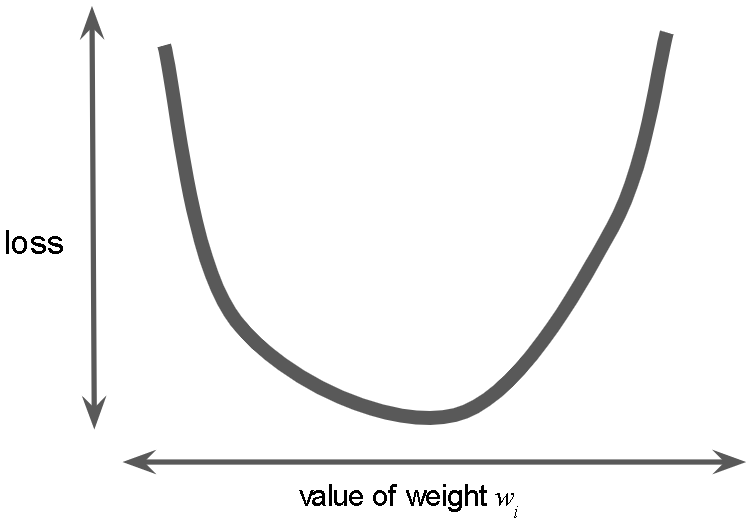
\includegraphics[width=0.5\textwidth]{fig/2-fundamentacao/aprendizado/convexo.png}
%             \fonte{}
%             \label{fig:convexo}
%         \end{figure}
        
%         Esse problema é muito simples, pois uma parábola possuí apenas um mínimo, ou seja, um lugar com inclinação exatamente igual a 0. Entretanto, por mais fácil que seja visualizar o ponto onde a função perda converge em uma parábola, ainda é um processo inviável e ineficiente, levantar todos os valores para posteriormente encontrar o mínimo.
        
%         Um método melhor e mais popular, no aprendizado de máquinas, é o gradiente descendente. Essa técnica também começa com um palpite para $b$ e $w_1$. O ponto de partida não importa muito, assim, muitos algoritmos simplesmente configuram para iniciar em 0 ou em um valor aleatório, como exemplo, a Figura~\ref{fig:gradiente_descendente_ponto_inicial}. 

%         \begin{figure}[H]
%             \centering
%             \caption{Ponto de partida aleatório utilizado pelo gradiente descente para minimizar a perda.}
%             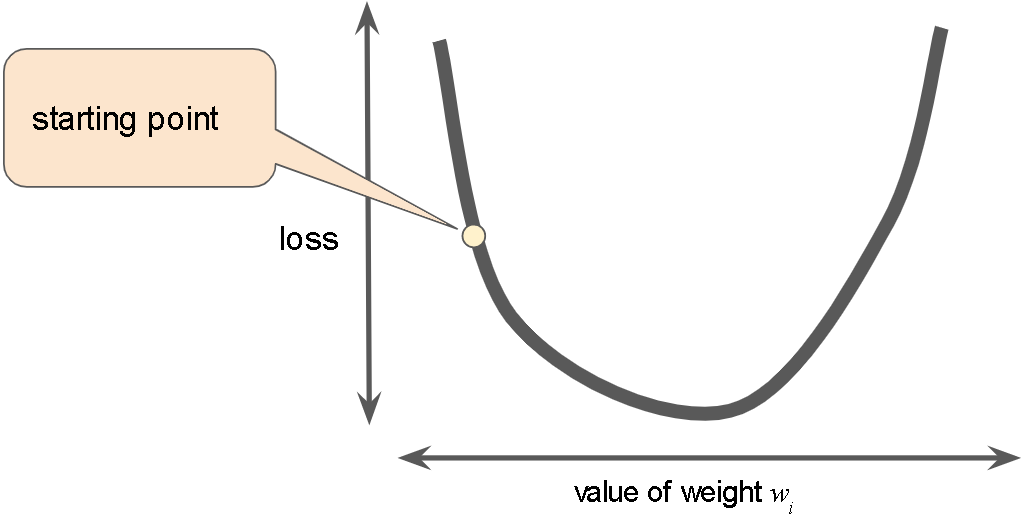
\includegraphics[width=0.5\textwidth]{fig/2-fundamentacao/aprendizado/gradiente_descendente_ponto_inicial.png}
%             \fonte{}
%             \label{fig:gradiente_descendente_ponto_inicial}
%         \end{figure}
        
%         O algoritmo calcula o erro no ponto inicial pela derivada parcial, que informa o quanto a função muda quando é feita uma pequena perturbação em uma variável, num peso. Com base nesta variação, o gradiente consegue predizer se a inclinação da derivada é positiva ou negativa. Como o intuito é encontrar o mínimo, a rede seguirá o gradiente negativo, conhecido como gradiente descendente. Quando há vários pesos, o gradiente é um vetor de derivadas parciais em relação aos pesos. Como o gradiente é um vetor, ele tem uma direção e uma magnitude, seu resultado sempre aponta na direção do gradiente negativo para reduzir a perda o mais rápido possível, como mostra a Figura~\ref{fig:vetor_direcao_gradiente}. 

%         \begin{figure}[H]
%             \centering
%             \caption{A descida do gradiente depende de gradientes negativos.}
%             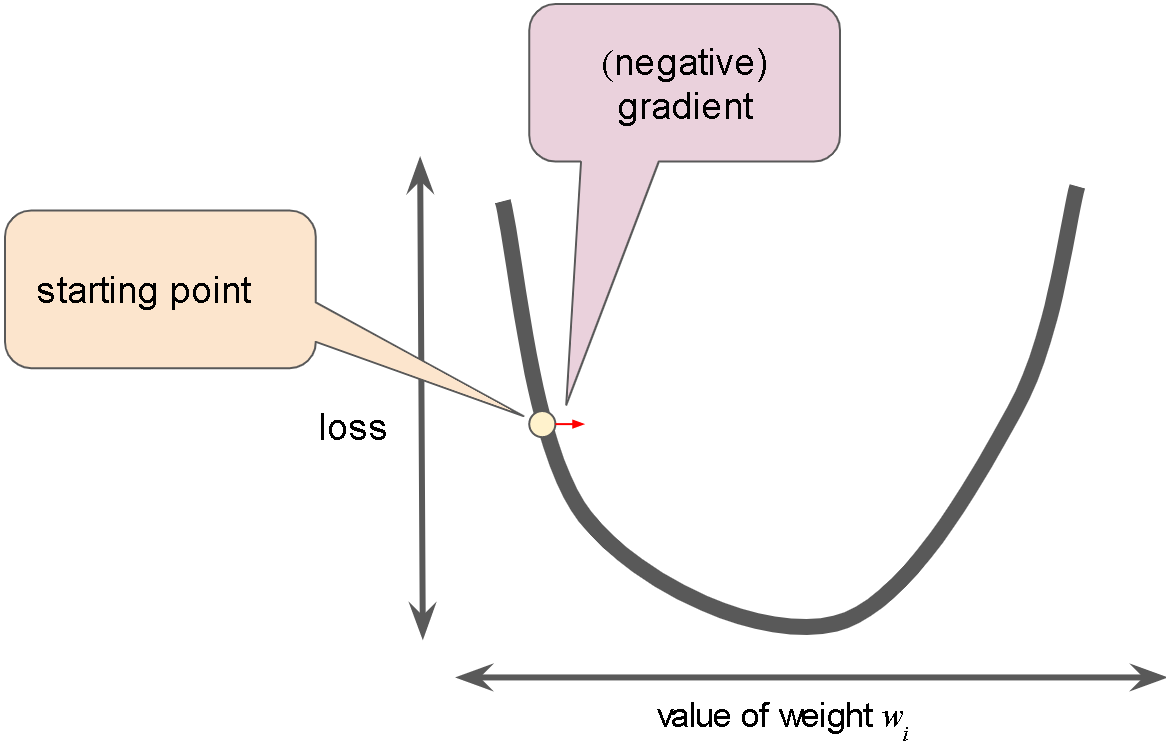
\includegraphics[width=0.5\textwidth]{fig/2-fundamentacao/aprendizado/vetor_direcao_gradiente.png}
%             \fonte{}
%             \label{fig:vetor_direcao_gradiente}
%         \end{figure}
        
%         Para determinar o próximo ponto ao longo da curva de perda, o algoritmo adiciona uma fração da magnitude do gradiente ao ponto inicial, conforme mostrado na Figura~\ref{fig:vetor_magnitude_gradiente}. Esse processo é repetido, chegando cada vez mais perto do mínimo. 

%         \begin{figure}[H]
%             \centering
%             \caption{Acréscimo da magnitude do gradiente no valor do ponto inicial move para o próximo ponto da curva de perda.}
%             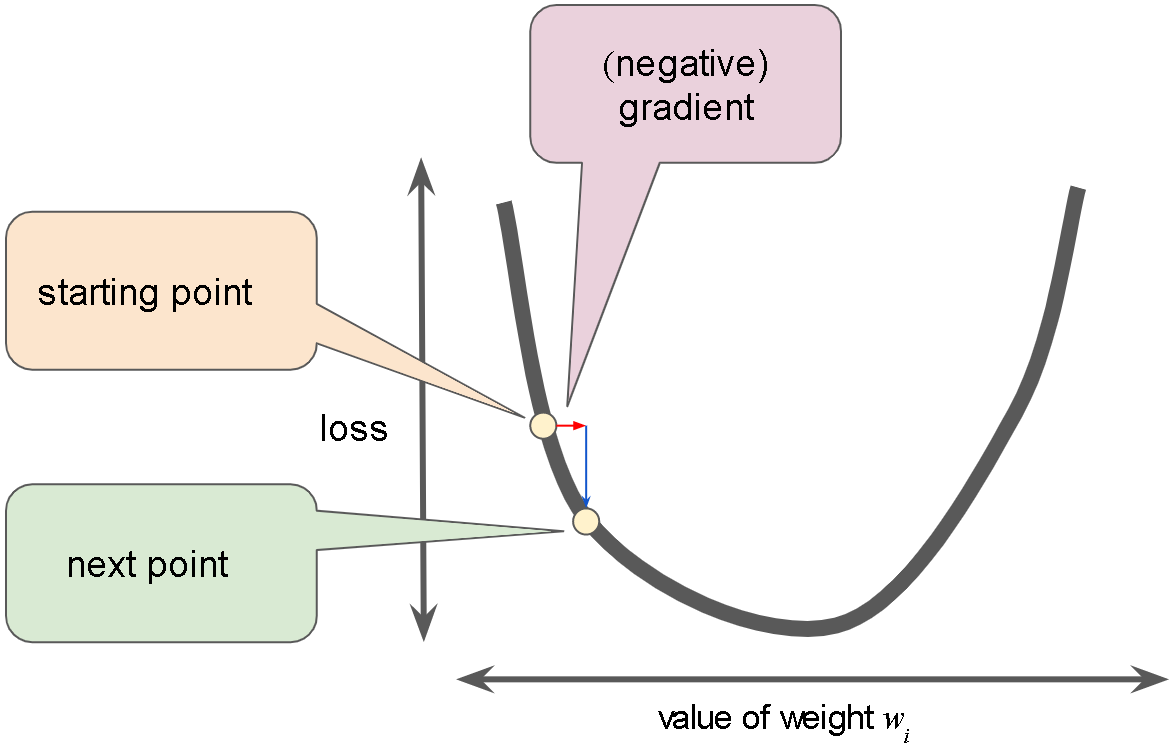
\includegraphics[width=0.5\textwidth]{fig/2-fundamentacao/aprendizado/vetor_magnitude_gradiente.png}
%             \fonte{}
%             \label{fig:vetor_magnitude_gradiente}
%         \end{figure}
        
%         Entretanto, não é somente somado ao ponto inicial o valor da magnitude, antes disso, ela é multiplicada pala taxa de aprendizado, também chamado de tamanho do passo. A taxa de aprendizado é um hiper parâmetro, ou seja, uma das variáveis que controla o próprio processo de treinamento. Esse conjunto soma e multiplicação que realmente dita o próximo ponto de análise na função de perda. Para exemplificar, considere uma magnitude de 2,5 e uma taxa de 0,01, o algoritmo escolherá o próximo ponto a uma distancia de 0,025 do valor anterior.
        
%         A taxa de aprendizado trás algumas informação importante, se ela for muito pequena, o treinamento demorará muito como mostra a Figura~\ref{fig:taxa_pequena}. Por outro lado, se ela for muito grande, o ponto irá saltar perpetuamente ao acaso perto do vale sem convergir, demonstrado pela Figura~\ref{fig:taxa_grande}. 

%         \begin{figure}[H]
%             \centering
%             \caption{A taxa de aprendizagem é muito pequena.}
%             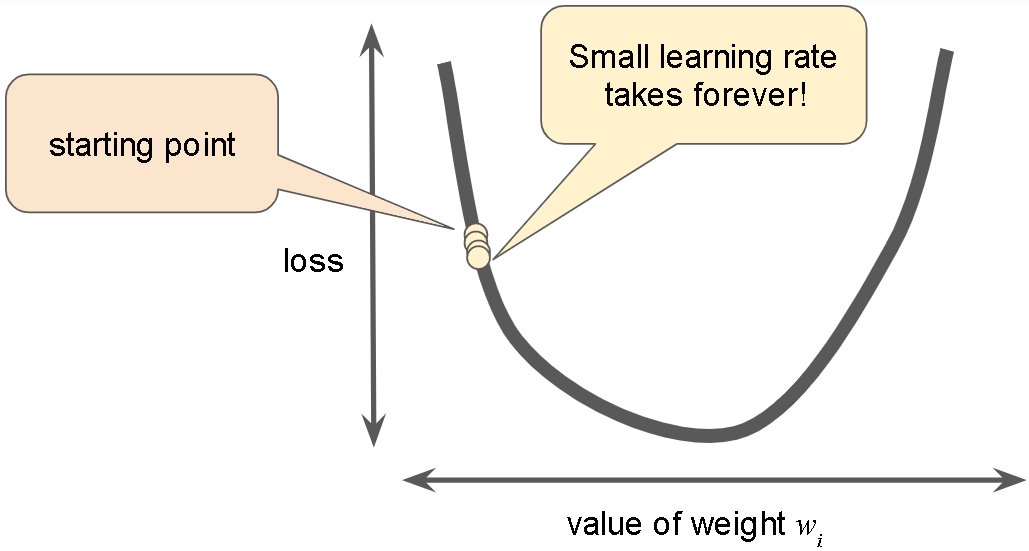
\includegraphics[width=0.5\textwidth]{fig/2-fundamentacao/aprendizado/taxa_pequena.png}
%             \fonte{}
%             \label{fig:taxa_pequena}
%         \end{figure}
        
%         \begin{figure}[H]
%             \centering
%             \caption{A taxa de aprendizagem é muito grande.}
%             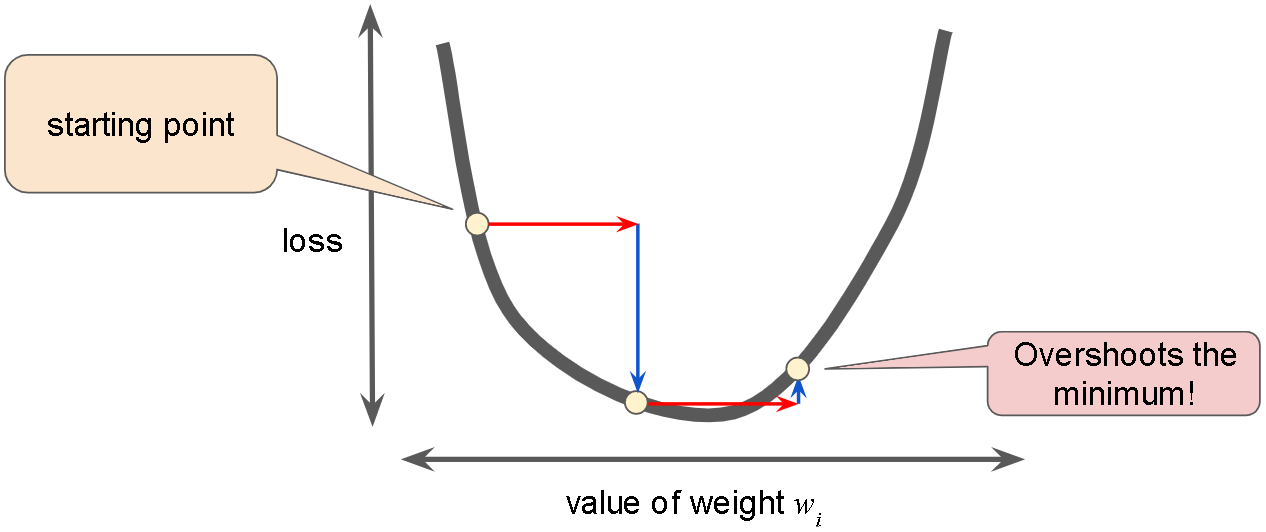
\includegraphics[width=0.5\textwidth]{fig/2-fundamentacao/aprendizado/taxa_grande.png}
%             \fonte{}
%             \label{fig:taxa_grande}
%         \end{figure}
        
%         Existe uma taxa de aprendizagem \textit{Goldilocks} para cada problema de regressão, que descreve o quão plana é a função de perda. Essa informação permite aumentar com segurança a taxa de aprendizado, se for de conhecimento prévio que o gradiente é pequeno. Com essa compreensão que o valor da magnitude do gradiente é pequeno, possibilita configurar um tamanho de passo maior, e dessa forma, que a perda encontre o mínimo no menor número de etapas. Já a taxa de aprendizagem ideal em uma dimensão é o inverso da segunda derivada de $f(x)$ em $x$ e para 2 ou mais dimensões é o inverso da matriz das derivadas parciais secundárias. 
        
%         Uma terminologia importante, no gradiente descendente, é \textit{batch} (lote) definido como o número total de exemplos usados para calcular o gradiente em uma única iteração. Quando é dado como entrada para o calculo da inclinação o conjunto inteiro de dados, considera-se que foi utilizado um \textit{batch}. Entretanto, eles geralmente contêm um grande número de \textit{features}, ou seja, um lote pode ser enorme, fazendo com que até mesmo uma única iteração demore muito para ser computada.

%         % % NÃO SEI SE USEI SGD - SE TIVER USADO OLHAR ESTE TEXTO EM COMENTÁRIO E ADICIONAR AO DOCUMENTO FINAL

%         % Um grande conjunto de dados com exemplos de amostra aleatória provavelmente contém dados redundantes, na verdade, isto se torna mais provável à medida que o tamanho do lote aumenta. Alguma redundância pode ser útil para suavizar gradientes ruidosos, mas lotes enormes tendem a não ter muito mais valor preditivo do que \textit{batch} grandes.
        
%         % É possível obter o gradiente correto, em média, com muito menos computação. Para isso, escolhe-se exemplos aleatoriamente no conjunto de dados, estimando (embora ruidosamente) uma grande média a partir de uma muito menor. A Stochastic gradient descent (SGD, gradiente descendente estocástico) leva essa ideia ao extremo - usa apenas um único exemplo (um tamanho de lote de 1) por iteração. Com iterações suficientes, o SGD funciona, mas é muito barulhento. O termo "estocástico" indica que o único exemplo que compreende cada lote é escolhido aleatoriamente.
        
%         % Mini-batch stochastic gradient descent (mini-batch SGD) é um meio-termo entre a iteração do lote completo e o SGD. Um minilote normalmente tem entre 10 e 1.000 exemplos, escolhidos aleatoriamente. O mini-lote SGD reduz a quantidade de ruído no SGD, e ainda é mais eficiente do que o lote completo.
        
%         % Para simplificar a explicação, focamos na descida do gradiente para um único recurso. Tenha certeza de que a descida gradiente também funciona em conjuntos de recursos que contêm vários recursos.
        
%     \section{\textit{Overfitting}, \textit{Underfitting} e \textit{split sample}}
    
%         Para descrever o que é \textit{overfitting},e \textit{underfitting} e o porque de separar os dados em subconjuntos, será usado outras amostras com somente uma \textit{feature}, apresentadas na Figura~\ref{fig:dados_simples}. Assim como no exemplo da seção anterior, o objetivo é desenvolver um modelo para prever os \textit{labels} e a partir dele discutir esses processos.

%         \begin{figure}[H]
%             \centering
%             \caption{Pequena amostra de dados com somente uma dimensão \textit{feature}.}
%             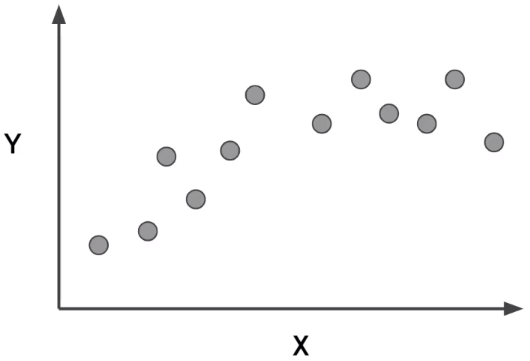
\includegraphics[width=0.5\textwidth]{fig/2-fundamentacao/overfitting/dados_simples.png}
%             \fonte{}
%             \label{fig:dados_simples}
%         \end{figure}

%         É considerado como um bom modelo, aquele que tenta se ajustar à tendência geral do conjunto de dados real, e não se encaixar perfeitamente neles. A Figura~\ref{fig:modelo_bom} exibe esse comportamento de generalizar seus resultados.

%         \begin{figure}[H]
%             \centering
%             \caption{Comportamento esperado para um bom modelo.}
%             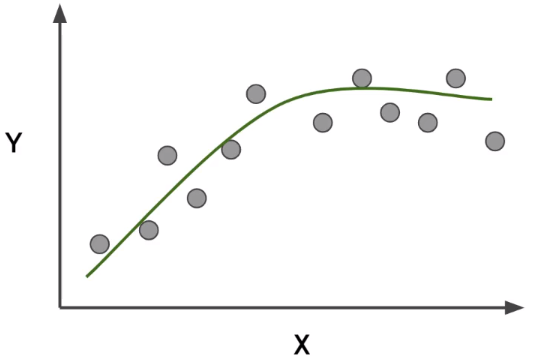
\includegraphics[width=0.5\textwidth]{fig/2-fundamentacao/overfitting/modelo_bom.png}
%             \fonte{}
%             \label{fig:modelo_bom}
%         \end{figure}
        
%         A Figura~\ref{fig:overfitting} apresenta o comportamento de um  modelo com \textit{overfitting} utilizando as amostras da Figura~\ref{fig:dados_simples}. Nela é possível ver que a curva passa exatamente em todos os pontos do gráfico, inclusive, ao ruído. Quando isso acontece, ele se torna mais complexo do que necessário, seu erro de treinamento é extremamente baixo ou, como neste caso específico, igual à zero.
        
%         % \textit{Overfitting} é quando o modelo se encaixa perfeitamente ao ruído nos dados, ou seja, . Isso geralmente resulta em baixo erro em conjuntos de treinamento, mas alto erro em seus conjuntos de teste e validação.

%         \begin{figure}[H]
%             \centering
%             \caption{Modelo considerado ruim com a presença de \textit{overfitting}.}
%             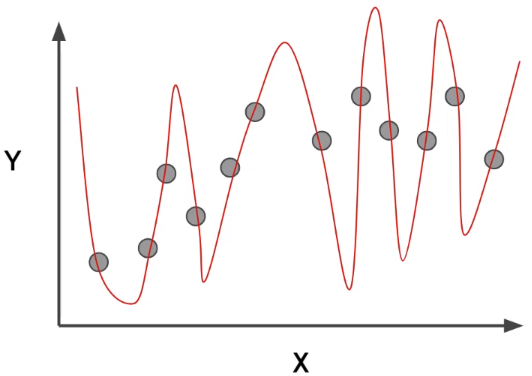
\includegraphics[width=0.5\textwidth]{fig/2-fundamentacao/overfitting/overfitting.png}
%             \fonte{}
%             \label{fig:overfitting}
%         \end{figure}
        
%         O oposto do \textit{overfitting} é o \textit{underfitting}, que ocorre em modelos excessivamente simples os quais não conseguem capturar a tendência dos dados para prever seu comportamento. Como resultado, frequentemente, apresentam baixa variança e alto bias. Um exemplo é apresentado na Figura~\ref{fig:underfitting}, ele também foi baseados nas amostras da Figura~\ref{fig:dados_simples}.
        
%         \begin{figure}[H]
%             \centering
%             \caption{Exemplo de um modelo considerado ruim por apresentar \textit{underfitting}.}
%             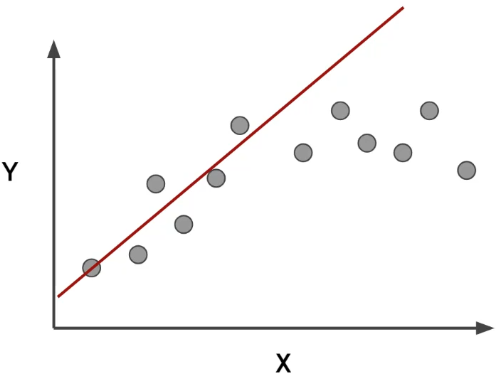
\includegraphics[width=0.5\textwidth]{fig/2-fundamentacao/overfitting/unterfitting.png}
%             \fonte{}
%             \label{fig:underfitting}
%         \end{figure}
        
%         % O objetivo do aprendizado de máquina é prever bem os novos dados extraídos de uma distribuição de probabilidade verdadeira (oculta).
%         Infelizmente, o modelo não consegue ver todas as informações possíveis, uma vez que, ele só recebe uma amostra de dados, denominado conjunto de treinamento. Isso acarreta em um problema, se ocorrer \textit{overfitting} ou \textit{underfitting} nos exemplos atuais, como confiar que o modelo também fará boas previsões sobre exemplos nunca antes vistos? Esse é o motivo de separar os conjuntos de dados em mais de um subconjunto, as separações mais utilizada em ML são:
        
%         % Esta segmentação pode ser feita nos seguintes grupos:
%         \begin{itemize}
%             \item Em duas divisões denominadas: treino e teste;
%             \item Em três divisões denominadas: treino, teste e validação.
%             % \item Em quatro divisões denominadas: treino, teste, validação e \textit{deployment}.
%         \end{itemize} 
        
%         O conjunto de teste deve atender à duas condições: ser grande o suficiente para produzir resultados estatisticamente significativos; ser representativo para o conjunto de dados como um todo, em outras palavras, não pode ser escolhido um conjunto de teste com características diferentes do conjunto de treinamento. 
        
%         Supondo que o conjunto de teste atenda às duas condições anteriores, independente de qual divisão for escolhida, haverá um subconjunto para tetar o modelo já treinado. Dessa forma, é possível avaliar se há \textit{overfitting} ou \textit{underfitting} a partir dos resultados do calculo de erro. Isso porque, este valor será pequeno para o conjunto de treinamento, mas para as novas amostras de teste será muito maior. A Figura~\ref{fig:teste_overfitting_novo_valor} apresenta a um ponto de teste.

%         \begin{figure}[H]
%             \centering
%             \caption{Novo valor teste aplicado a um modelo com \textit{overfitting}.}
%             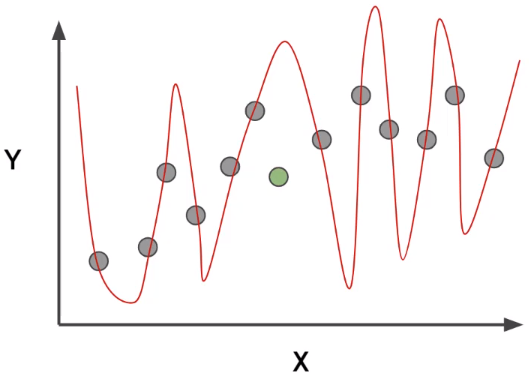
\includegraphics[width=0.5\textwidth]{fig/2-fundamentacao/overfitting/testando_overfitting.png}
%             \fonte{}
%             \label{fig:teste_overfitting_novo_valor}
%         \end{figure}
        
%         A noção da grandeza do erro pode ser visualizada na distância entre o ponto, valor real, e a curva, equação de inferência, como mostras a Figura~\ref{fig:erro_novo_valor}. Lembrando que, os valores de teste não podem ser utilizados durante o treinamento, garantindo assim, que o modelo não tenha visto antes estes dados.

%         \begin{figure}[H]
%             \centering
%             \caption{Apresenta distância entre o novo ponto e a predição do modelo, ou seja, uma visualização do erro.}
%             \includegraphics[width=0.5\textwidth]{fig/2-fundamentacao/overfitting/overfitting_erro_evaluate.png}
%             \fonte{}
%             \label{fig:erro_novo_valor}
%         \end{figure}

%         Considere a Figura~\ref{fig:teste_sem_overfitting}, nela esta representado o mesmo o modelo da Figura~\ref{fig:modelo_bom}, considerado bom, e o valor utilizado para teste na Figura~\ref{fig:teste_overfitting_novo_valor}. Por mais que o modelo seja muito simples e que não faça um trabalho perfeito (algumas previsões estão erradas), ele se sai tão bem nos dados de treinamento quanto no ponto de teste, ou seja, a equação não se ajusta demais nos dados de treinamento.
        
%         Um bom desempenho no conjunto de teste, indica o quanto que se pode confiar nos resultados obtidos com novos dados. Entretanto, isso só é válido se: o subconjunto de teste for grande o suficiente; e se não houver "trapaça", isto é, se o mesmo conjunto de teste não for usado repetidamente, ou no lugar do de treinamento. Esse último, pode-se ser concluído por métricas de avaliação com valores surpreendentemente bons, por exemplo, uma alta precisão pode indicar que os dados de teste vazaram para o conjunto de treinamento.
        
%         Outra forma de garantir a qualidade dos resultados é eliminando exemplos que acarretam problemas de aprendizado para o algoritmo. Como no caso de um modelo treinado para classificar \textit{e-mails} como sendo spam ou não, o qual as amostras foram distribuídos em treino e teste. Indiferente do resultado, o esperado é obter valores para as métricas menores no conjunto de teste, isso porque, o modelo não o usou como base de informações. 
        
%         Na hipótese dele atingir a mesma acurácia nos dois conjuntos, treinamento e teste, gera-se um alerta. Logo, os dados devem ser verificados novamente, e se por acaso, forem descobertos \textit{e-mail} duplicados, entre os dois subconjuntos, a abordagem ideal é remover essas entradas e redividi as amostras. Do contrário, não será possível afirmar o quão bem o modelo consegue se generalizar inferindo corretamente novos dados. %, no qual as amostras foram distribuídos em conjuntos de treinamento e teste com a divisão de 80-20
        
%         O fluxo de trabalho da divisão em dois conjunto, treino e teste, pode ser analisado na Figura~\ref{fig:fluxo_treino_teste}. Nela, a etapa \textit{"Tweak model"} descreve o momento no qual pode-se ajustar a rede, as possibilidades vão desde alterar a taxa de aprendizado, adicionar ou remover recursos, até projetar um modelo completamente novo do zero. No final deste fluxo de trabalho, escolhe-se o modelo que se sai melhor no conjunto de teste.

%         \begin{figure}[H]
%             \centering
%             \caption{Fluxo de trabalho para separação do conjunto de dados em treino e teste.}
%             \includegraphics[width=0.5\textwidth]{fig/2-fundamentacao/overfitting/fluxo_treino_teste.png}
%             \fonte{}
%             \label{fig:fluxo_treino_teste}
%         \end{figure}
        
%         Entretanto, deve-se observar que esse procedimento é uma abordagem simplificada, pois a divisão é feita somente em dois bloco, o que não é adequado para obter o desempenho final do modelo. Isso porque, é possível atualizar os parâmetros repetidas vezes após avaliar os resultados no conjunto de teste. Por causa disso, os dados costumam ser divididos em três conjuntos: treinamento, validação e teste.
        
%         % Essa última abordagem reduz significativamente as chances de ocorrer \textit{overfitting}. A segmentação de validação é usada para avaliar os resultados do conjunto de treinamento, e em seguida, os dados de teste são usados para verificar novamente a performance. Ou seja, é escolhido o modelo treinado que funcione melhor no conjunto de validação e posteriormente ele é verificado novamente em relação ao conjunto de teste. Nessa última etapa, é importante garantir que os dados de teste nunca antes tenham sido vistos pela rede neural. O fluxo de trabalho desta opção de segmentação das amostras é apresentada na Figura~\ref{fig:fluxo_treino_teste_validação}.
        
%         Essa abordagem reduz significativamente as chances de ocorrer \textit{overfitting}, pois, em resumo, as separações das amostra em 3 blocos são usadas da seguinte forma: com o conjunto para o treinamento o modelo consegue aprender as relações entre \textit{features} e \textit{labels} e assim ajustar-se aos dados. As amostras de validação, são aplicadas a rede para verificar o desempenho e ele é a referência nos ajuste do modelo (adição de neurônios ou camadas, mudança na arquitetura real da rede etc.). Repete-se esse processo até ter resultados que satisfação condições específicas. Só então, é possível avaliar o verdadeira performance do modelo com a ajuda da terceira divisão de dados, a de teste. Esse bloco é aplicado em métrica específicas para determinar o comportamento final, esperado no mundo real. É importante observar que após executar o modelo com os dados de teste não será mais possível voltar e refinar os hiper-parâmetros da rede. O fluxo de trabalho da divisão em três conjunto pode ser analisado na Figura~\ref{fig:fluxo_treino_teste_validação}.

%         \begin{figure}[H]
%             \centering
%             \caption{Fluxo de trabalho para separação do conjunto de dados em treino, teste e validação.}
%             \includegraphics[width=0.5\textwidth]{fig/2-fundamentacao/overfitting/fluxo_treino_teste_validação.png}
%             \fonte{}
%             \label{fig:fluxo_treino_teste_validação}
%         \end{figure}
        
%         Até agora, as explicações foram realizadas com base em problemas de uma única \textit{feature}, pois são de fácil visualização. Entretanto, isso não ocorre frequentemente no mundo real, o qual na maior parte do tempo trabalha-se com \textit{datasets} multidimensionais, que necessitam de uma abordagem diferente. Para discutir o melhor procedimento, considere a Figura~\ref{fig:erro_tempo_treinamento} que apresenta a relação: medição do erro versus tempo de treinamento de um modelo considerado ideal.
        
%         \begin{figure}[H]
%             \centering
%             \caption{Modelo ideal em relação ao erro versus tempo de treinamento.}
%             \includegraphics[width=0.5\textwidth]{fig/2-fundamentacao/overfitting/multidimencional_treinamento.png}
%             \fonte{}
%             \label{fig:erro_tempo_treinamento}
%         \end{figure}
        
%         Ao aplicar os dados de treinamento pela primeira vez no modelo, o valor de perda obtido será grande. Isso porque, o algoritmo não teve acesso a essas informações antes e ajustou quaisquer parâmetros internos como hipótese inicial. No entanto, conforme ocorre o aprendizado, ou seja, quanto mais tempo de treinamento, espera-se que o erro diminua até que se estabilize e converta para algum tipo de mínimo.
        
%         No caso de redes neurais, este tempo de treinamento tem uma denominação específica, época. Essencialmente, uma época ocorre quando a totalidade dos dados de treinamento passa pelo modelo. Esse procedimento acontece várias vezes até que obtém-se um bom modelo, como mostra a Figura~\ref{fig:epoch}. % erro convergirá para algum tipo de mínimo o
        
%         \begin{figure}[H]
%             \centering
%             \caption{Modelo ideal em relação ao erro versus epochs.}
%             \includegraphics[width=0.5\textwidth]{fig/2-fundamentacao/overfitting/epoch.png}
%             \fonte{}
%             \label{fig:epoch}
%         \end{figure}
        
%         Um modelo péssimo, apresenta erros crescentes a medida que o tempo passa, ou seja, o modelo não aprende a cada época. Esse comportamento é demonstrado pela Figura~\ref{fig:modelo_ruim}.
        
%         \begin{figure}[H]
%             \centering
%             \caption{Modelo ruim em relação ao erro versus epochs.}
%             \includegraphics[width=0.5\textwidth]{fig/2-fundamentacao/overfitting/modelo_ruim.png}
%             \fonte{}
%             \label{fig:modelo_ruim}
%         \end{figure}
        
%         Portanto, o estudo da simplicidade/complexidade dos modelos é importe para compreender a relação entre o desempenho deles nos conjuntos de treino e de teste/validação, sendo possível visualizar esse comportamento conforme as épocas passam. A Figura~\ref{fig:epocas_treino_teste} mostra o resultado ideal obtidos durante o treinamento, curva em vermelho, e de o teste, curva em azul.
        
%         \begin{figure}[H]
%             \centering
%             \caption{Modelo ideal de erro de treino e de teste em relação ao as \textit{epochs}.}
%             \includegraphics[width=0.5\textwidth]{fig/2-fundamentacao/overfitting/epocas_treino_teste.png}
%             \fonte{}
%             \label{fig:epocas_treino_teste}
%         \end{figure}
        
%         No comportamento ideal, tanto o conjunto de treino como o de teste tem seu erro reduzido a medida que as épocas passam. O resultado deles é similar, entretanto, no teste espera-se valores de perda maiores. Agora, se há \textit{overfitting}, ao testa-los, tanto com os dados de teste como com os de validação, o resultado será ruim, isso pode ser analisado na Figura~\ref{fig:Epoca_teste_ruim}.
        
%         \begin{figure}[H]
%             \centering
%             \caption{Modelo ruim de erro de treino e de teste em relação ao as \textit{epochs}.}
%             \includegraphics[width=0.5\textwidth]{fig/2-fundamentacao/overfitting/Epoca_teste_ruim.png}
%             \fonte{}
%             \label{fig:Epoca_teste_ruim}
%         \end{figure}
        
%         O exemplo da Figura~\ref{fig:Epoca_teste_ruim} é uma boa indicação de complexidade excessiva nos dados de treino. Nela é possível visualizar o ponto no conjunto de teste, no qual o erro em vez de diminuir começa a aumentar. Esse ponto define quando parar de treinar o modelo, pois, para as épocas a seguir começará o \textit{overfitting} e os resultados para novos dados serão piores. Esse ponto de corte é apresentado na Figura~\ref{fig:ponto_de_corte}.
        
%         \begin{figure}[H]
%             \centering
%             \caption{Ponto de corte no tempo de treinamento para evitar \textit{overfitting}.}
%             \includegraphics[width=0.5\textwidth]{fig/2-fundamentacao/overfitting/ponto_de_corte.png}
%             \fonte{}
%             \label{fig:ponto_de_corte}
%         \end{figure}
        
%     \section{Avaliando o desempenho - Métricas de erro de classificação}\label{cap:metrica}
        
%         Este capítulo descreverá as métricas de avaliação de desempenho para problemas de classificação. Elas são utilizadas no final do processo de aprendizado, após o treinamento, com os dados do conjunto de teste e servem para avaliar como o modelo realmente performou. 
        
%         As principais métricas de classificação estudadas por este trabalho são: acurácia (\textit{accuracy}), recall, precisão (\textit{precision}) e F1-Score. Antes de descrever-las, será explicado o raciocínio por trás delas e como realmente funcionam no mundo real. 
        
%         Em uma típica tarefa de classificação, o modelo pode alcançar apenas dois resultados: ou ele realizou uma previsão correta; ou ele realizou uma previsão incorreta. Todas as métricas de classificação derivam dessa ideia, e felizmente, é possível expandi-la para situações em que há várias classes, entretanto, para explicar o propósito delas será considerado uma classificação binária.
        
%         A partir de um modelo que tem como objetivo classificar imagens como sendo de cachorro ou de gato, será descrito como determinar o desempenho real/final. O conjunto de teste possuí \textit{features}, $x_{\text{test}}$, imagens de cachorro e gato, e seus respectivos \textit{labels}, $y_{\text{test}}$, o nome cachorro e gato. 
        
%         As imagens são dadas como entrada no modelo já treinado, que faz uma previsão, este resultado será uma predição correta, por exemplo, se a rede inferir cachorro para uma imagem de cachorro, como mostra a Figura~\ref{fig:cao_igual_cao}. 
        
%         % , então, a inferência é comparadas com o \textit{label} correto obtendo um valor de erro.
    
%         \begin{figure}[H]
%             \centering
%             \caption{Predição correta da rede neural.}
%             \includegraphics[width=0.5\textwidth]{fig/2-fundamentacao/metricas/cao_igual-cao.png}
%             \fonte{}
%             \label{fig:cao_igual_cao}
%         \end{figure}
        
%         Porém, ela estará incorreta quando seu \textit{output} for gato e a imagem é de um cachorro, resultado apresentado pela Figura~\ref{fig:gato_nao_igual_cao}. 
    
%         \begin{figure}[H]
%             \centering
%             \caption{Predição incorreta da rede neural.}
%             \includegraphics[width=0.5\textwidth]{fig/2-fundamentacao/metricas/gato_nao_igualcao.png}
%             \fonte{}
%             \label{fig:gato_nao_igual_cao}
%         \end{figure}
        
%         Ao repetir esse processo para todas as imagens do banco de dados de teste, tem-se uma contagem das correspondências corretas e incorretas. É importante dizer que, no mundo real, nem todas as correspondências incorretas ou corretas têm o mesmo valor. Isso significa que, uma única métrica não é o suficiente para caracterizar o desempenho do modelo. Portanto, utiliza-se as quatro métricas e organiza-se os valores previstos em comparação com os reais no que é conhecido como matriz de confusão.
        
%         A matriz de confusão apresenta os resultados de classificações corretas versus incorretas, como mostra a Figura~\ref{fig:matriz_confusão}. As condições verdadeiras (\textit{True Condition}) que indicam qual o \textit{label} correto/esperado para um dada inferência. Essas condições possuem duas subcategorias, positiva e negativa, em outras palavras, é realmente cachorro versus não é. As inferência realizadas pelo modelo são apontadas na condições de predição (\textit{predicted condition}), que também podem assumir duas categorias, positiva e negativa.
        
%         % Muitas vezes, é usado para diagnóstico médico, descrevendo se existe a presença de uma doença contra não existe. 
    
%         \begin{figure}[H]
%             \centering
%             \caption{Matriz de confusão na qual computa predições em relação do que se esperava como \textit{output}.}
%             \includegraphics[width=0.5\textwidth]{fig/2-fundamentacao/metricas/matriz_confusão.png}
%             \fonte{}
%             \label{fig:matriz_confusão}
%         \end{figure}
        
%         Como é possível analisar, os elementos da diagonais da matriz apresentam as previsões corretas para diferentes classes, enquanto os dados fora da diagonal mostram as amostras que foram mal classificadas. Assim as possibilidades de resultados de classificações são:
%         \begin{itemize}
%             \item verdadeiro positivo (\textit{true positive} - TP): o modelo prediz corretamente a classe positiva;
%             \item verdadeiro negativo (\textit{true negative} - TN): o modelo prediz corretamente a classe negativa;
%             \item falso positivo (\textit{false positive} - FP): o modelo prediz incorretamente a classe positiva (erro tipo 1);
%             \item falso negativo (\textit{false negative} - FN): o modelo prediz incorretamente a classe negativa (erro tipo 2).
%         \end{itemize}\\
        
%         Considerando como classe positiva a imagem de cachorro e a negativa a de gato, tem-se os seguintes resultados:
%         \begin{itemize}
%             \item TP: é a imagem de um cachorro e o modelo predisse corretamente cachorro;
%             \item TN: é a imagem de um gato e o modelo predisse corretamente gato;
%             \item FP: é a imagem de um cachorro e o modelo predisse incorretamente gato;
%             \item FN: é a imagem de um gato e o modelo predisse incorretamente cachorro;
%         \end{itemize}
        
%         A partir das informações discutidas até aqui, é possível compreender as métricas, começando pela acurácia, que pode ser calculada pela média dos valores situados na "diagonal principal". Neste caso, ela é escrita em termos de positivos e negativos como mostra a equação~\ref{eq:acuracia_positivo_negativo}
        
%         \begin{equation}
%             \centering
%             \text{Acurácia} = \frac{TP + TN}{TP + TN + FP + FN}
%             \label{eq:acuracia_positivo_negativo}
%         \end{equation}
        
%         Frequentemente é definida como o número de previsões corretas feitas pelo modelo dividido pelo número total de predições, descrito pela equação~\ref{eq;acurácia}. Independente da forma escolhida para representa-la, a acurácia responde a pergunta, quantas predições corretas o modelo acertou em porcentagem. Por exemplo, um modelo terá uma acurácia de 80$\%$ se em um conjunto de testes com 100 imagens ele prever corretamente 80 delas. 
        
%         \begin{equation}
%             \centering
%             \text{Acurácia} = \frac{\text{Número de predições corretas}}{Número total de predições}
%             \label{eq:acuracia}
%         \end{equation}
        
%         O problema dessa métrica, é que ela é eficaz somente quando as classes alvo são bem balanceadas, isto é, sempre que há aproximadamente a mesma quantidade de imagens nas diferentes categorias. Mas em situações com desequilíbrio, ela é péssima para determinar o desempenho. Para entender o significado disso, considere um conjunto de teste com 99 imagens de cães e apenas uma de gato, e um modelo de uma linha que sempre irá prevê cachorro. A acurácia neste caso é de 99 $\%$, porque o único \textit{output} desta rede é cachorro, não importando a imagem dada a ela, e existem 99 imagens deles. Do contrário, se fosse uma reta constante na classe gato, o calculo resultaria em 1 $\%$ de acurácia, pois existe somente uma imagem deste animal. O motivo de utilizar outras métricas é porque na maior parte das situações trabalha-se com desigualdade de \textit{labels}.
        
%         Entre as métricas utilizadas com classes desbalanceadas estão recall e precisão. A primeira é definida como a capacidade de um modelo encontrar todos os casos relevantes dentro de um conjunto de dados, sua definição precisa é dado pela equação~\ref{eq:recall}. Essa métrica tenta responder a pergunta: Qual proporção de positivos reais foi identificada corretamente? 
        
%         \begin{equation}
%             \centering
%             Recall = \frac{TP}{TP + FN}
%             \label{eq:recall}
%         \end{equation}
        
%         Já a precisão é a capacidade de um modelo de classificação identificar apenas os pontos de dados relevantes, sendo descrita matematicamente pela equação~\ref{eq:precisão}. O objetivo dela é responder a pergunta: Qual proporção de identificações positivas estava realmente correta?
        
%         \begin{equation}
%             \centering
%             Recall = \frac{TP}{TP + FP}
%             \label{eq:precisão}
%         \end{equation}
        
%         Constantemente, há a necessidade de encontrar o equilíbrio entre recall e precisão, para isso usa-se uma combinação delas que é conhecida como F1-Score. Ela é obtida através a média harmônica entre essas duas métricas, de acordo com a equação~\ref{eq:F1Score}. A F1-Score informa o quão preciso é o classificador (quantas instâncias ele classifica corretamente), bem como, o quão robusto ele é (se ele não perde um número significativo de instâncias).
        
%         \begin{equation}
%             \centering
%             F1-Score = 2\cdot\frac{precision \cdot recall}{precision + recall}
%             \label{eq:F1Score}
%         \end{equation}
        
%         A razão para utilizar a média harmônica em vez da simples, é porque essa pune diferenças extremas. Por exemplo, se um classificador tem uma precisão igual à 1 (perfeita) e o recall igual à zero (pior registro possível), com a média simples o resultado é igual a 0,5, já estimado com o F1-Score a solução é 0. Então, pode-se notar que F1-Score penaliza desproporções grandes de precisão e recall e portanto, é uma avaliação mais justa, principalmente para classes desbalanceadas. 
        
%         A matriz de confusão e as várias métricas calculadas são maneiras de comparar o valor predito com o verdadeiro. Mas uma pergunta relevante é, qual dessas métricas é a "ideal"? A reposta depende da situação na qual o modelo está sendo executado, e do contexto do problema. Não existe um número único e mágico, que se possa afirmar que é o melhor. Por exemplo, não é possível declarar que $99\%$ de acurácia é bom o suficiente para todas as situações, já que para classes desbalanceadas isso não se aplica. A mesma observação vale para precisão e recall, pois, ao ajustar o resultado para diminuir um, o outro será aumentado. Ou seja, precisa-se decidir se o modelo deve se concentrar na correção de falsos positivos ou nos de falsos negativos. Essa constatação pode ser exemplificada ao substituir o exemplo da classificação de imagens por a de diagnóstico de doença. 
        
%         No problema de predição de doenças, dificilmente haverá uma enfermidade que cerca de metade da população seja afetada e a outra não, logo, é um problema de classes desbalanceadas. Isso causa um "cobertor curto" entre precisão, que diminuindo melhora os FP, e recall, que diminuindo melhora os FN. É importante ressaltar que, modelos de inteligência artificial, em situações de problemas de saúde são usados como diagnóstico rápido antes de realizar um exame mais invasivo, pois, na investigação de patologias mais severas, as "apostas" são altas. Neste caso, é melhor tentar minimizar o número de falsos negativos ao custo de aumentar o de falsos positivos. para se ter certeza de que foram classificados corretamente o maior quantidade possível de casos. 
        
%         Portanto, o ideal nesta cenário é que todas as pessoas doentes passem para a próxima etapa, isso é muito importante, pois os modelos de inteligência artificial não são perfeitos. Dessa forma, é melhor diagnosticar uma pessoa como enfermar e garantir que ela siga sendo acompanhada para no futuro, com outros exames, possa ser dispensada como um diagnóstico errado, do que não tratar uma pessoa enferma. Isso considerando que haverão testes complementares, que por mais invasivos possam confirmaram ou não esse resultado prévio. O oposto é verificado na fabricação de equipamento, onde prefere-se que máquinas sem defeito sejam descartadas (FP) do que as com mau funcionamento sejam entregues ao consumidor final (FN).
        
%         Existem outras métricas calculáveis que tentam prever o desempenho de modelos, entretanto, este trabalho irá abordar somente as descritas neste capítulo. Para mais informação sobre outras possibilidade de determinar a performance podem ser estudadas em\todo{citar bibliografia wikipédia}. 
    
        
%     \section{Regressão logística para classificação binária}
    
%         Muitos problemas requerem uma estimativa de probabilidade como saída. A regressão logística é um mecanismo extremamente eficiente para o cálculo de probabilidades. Em termos práticos, pode-se usar o resultado da probabilidade de uma das seguintes maneiras: como é; ou convertido em uma categoria binária.
        
%         Usando sem alteração, "como está", é calculado pela probabilidade de $A$ ocorrer dado $B$, definido por~\ref{eq:probabilidade_A|B}.
        
%         \begin{equation}
%             \centering
%             p(A|B)
%             \label{eq:probabilidade_A|B} 
%         \end{equation}
        
%         É possível converter o resultado da probabilidade para um valor binário, ou seja, para uma classificação (tema deste trabalho). Isso é realizado a partir de um limiar, também conhecido por limite de decisão, que define quando um valor de probabilidade passa de uma categoria para outra.
        
%         Para garantir que a saída do modelo de regressão logística fique entre 0 e 1, é usado uma função sigmoide, que produz o seguinte gráfico, apresentado na Figura~\ref{fig:sigmoide}. 
    
%         \begin{figure}[H]
%             \centering
%             \caption{Função sigmoide.}
%             \includegraphics[width=0.5\textwidth]{fig/2-fundamentacao/aprendizado/sigmoide.png}
%             \fonte{}
%             \label{fig:sigmoide}
%         \end{figure}
        
%         Se $z$ representa a saída da camada linear de um modelo treinado com regressão logística, então sigmoide ($z$) produzirá um valor (uma probabilidade) entre 0 e 1, dado pela equação~\ref{eq:sigmóide}. 
        
%         \begin{equation}
%             \centering
%             y = \frac{1}{1 + \exp^{-z}}
%             \label{eq:sigmóide}
%         \end{equation}
        
%         \begin{enumerate}\label{fig:MSE}
%             \item[] em que:
%             \begin{itemize}
%                 \item $y'$ é a saída do modelo de regressão logística para um exemplo específico;
%                 \item $z = b + w_{1}x_{1} + w_{2}x_{2} + ... + w_{N}x_{N}$
%                 \begin{itemize}
%                     \item $w$ são os pesos aprendidos pelo modelo;
%                     \item $b$ é o bias aprendido pelo modelo;
%                     \item $x$ são as \textit{features} para um exemplo específico.
%                 \end{itemize}
%             \end{itemize}
%         \end{enumerate}
        
%         $Z$ também é conhecido como \textit{log-odds} porque o inverso da sigmoide, dado pela equação~\ref{eq:inverso_sigmóide}. Ele afirma que, $z$ pode ser definido como o \textit{log} da probabilidade de "1" \textit{label} dividido pela probabilidade do "0" \textit{label}.
        
%         \begin{equation}
%             \centering
%             z = \log(\frac{y}{1 - y})
%             \label{log_odds}
%         \end{equation}
        
%         Para exemplificar, considere um modelo de regressão logística que recebera como paramenteiros de entrada os seguintes valores e \textit{features}:
        
%         \begin{itemize}
%             \item bias: $b = 1$;
%             \item peso 1, 2 e 3: $w_{1}$, $w_{2}$ e $w_{3}$;
%             \item \textit{features} 1, 2 e 3: 0, 10 e 2.
%         \end{itemize}
        
%         $z$ é dado pelo desenvolvimento a segui:
%         \begin{equation*}
%             z = b + w_{1}x_{1} + w_{2}x_{2} + w_{3}x_{3}
%         \end{equation*}
        
%         \begin{equation*}
%             z = 1 + 2\cdot0 + (-1)\cdot10 + 5\cdot2
%         \end{equation*}
        
%         \begin{equation*}
%             z = 1
%         \end{equation*}
        
%         Substituindo $z = 1$ na equação~\ref{eq:sigmóide}, obtém-se o seguinte resultado demonstrado pela Figura~\ref{fig:probabilidade_output}: 
        
%         \begin{equation*} 
%             \centering
%             y = \frac{1}{1 + \exp^{-1}}
%         \end{equation*}
        
%         \begin{equation*} 
%             y = 0,731
%         \end{equation*}
    
%         \begin{figure}[H]
%             \centering
%             \caption{Saída da regressão logística.}
%             \includegraphics[width=0.5\textwidth]{fig/2-fundamentacao/aprendizado/probabilidade_output.png}
%             \fonte{}
%             \label{fig:probabilidade_output}
%         \end{figure}
        
% % ADAPTAR ESTA SUBSECTION - TAREFA SUPERVISIONADA - COMO INICIO DE METODOLOGIA UTILIZADA, ACHO QUE NA METODOLOGIA ESTOU PINGANDO NO MOLHADO
% % \subsection{Tarefa supervisionada}
    
% %     Nesta seção será descrito os procedimentos que englobam o treinamento de um modelo de \textit{supervised machine learning}. O diagrama com as etapas que compõem o aprendizado é apresentado na Figura~\ref{fig:diagrama_supervised_ML}. Nele é possível ver as etapas de aquisição, formatação (pré-processamento) e separação dos dados em blocos, como também os procedimentos de treinamento, avaliação da performance do modelo (teste) e \textit{deployment}, este último, momento no qual ele é então aplicado na solução do problema real.

% %     % \begin{figure}[H]
% %     %     \centering
% %     %     \includegraphics[width=0.5\textwidth]{fig/sharpPonderacao.png}
% %     %     \caption{Esquemático de comparação entre label examples e a inferência da rede neural para o estimativa do erro.}
% %     %     \label{fig:diagrama_supervised_ML}
% %     % \end{figure}

% %     % Para sintetizar o funcionamento de uma rede neural supervisionada, considera-se um banco de dados, chamado de \textit{dataset}, o qual contem um histórico de \textit{features} e de seus respectivos \textit{labels}, ou seja, se tem conhecimento prévio do \textit{output} para um dado \textit{input}. %Essa é a principal a plicação das as redes supervisionadas, em problemas que se tem histórico de dados conhecido. 
    
% %     % A \textit{network} recebe uma parte desses dados, $(x,y)$, para o treinamento do modelo. Neste processo o algoritmo realiza uma comparação entre o \textit{label} predito (inferido) pela rede, representado pela variável $y'$, com o \textit{label} correto (verdadeiro). O erro é calculado através da diferença entre $y$ e $y'$ e é usado para alterar o modelo. Essas modificações podem ser, por exemplo, um ajuste dos pesos ou valor bias da network, etc., como também pode-se optar mudar a arquitetura da rede neural.
    
% %     % Na Figura(ref) é possível analisar o esquemático dos passos de desenvolvimento de uma rede supervisionada. 

% %     % \begin{figure}[H]
% %     %     \centering
% %     %     \includegraphics[width=0.5\textwidth]{fig/sharpPonderacao.png}
% %     %     \caption{Esquemático de comparação entre label examples e a inferência da rede neural para o estimativa do erro.}
% %     %     \label{fig:compLEeYlinha}
% %     % \end{figure},

% %     O primeiro procedimento, descrito no diagrama, é o de aquisição de dados, que depende do domínio no qual pretende-se trabalhar. No aprendizado supervisionado, se tem conhecimento prévio do \textit{output} para um dado \textit{input}. Com o \textit{dataset} determinado, realiza-se uma limpeza e formatação das amostras para que a rede neural possa realmente processá os \textit{inputs}. Então, os dados são divididos em um conjunto chamado treinamento e outro de teste determinado por uma proporção, na qual o maior bloco é destinado ao treinamento.

% %     O conjunto de dados de treinamento ajusta o modelo durante o aprendizado da rede. Já o separado para teste, é usado para calcular informações sobre a  performance do modelo treinado. A comparação entre $y$ e $y'$ descrita, utiliza métricas específicas e diferentes para cada tipo de problema. 
    
% %     A partir do desempenho, é possível determinar a necessidade de ajustar os parâmetros do modelo, como adicionar mais camadas ou mais neurônios na tentativa de obter um melhor ajuste nesse dados de teste. Uma vez que for considerado satisfatório os resultados, pode-se implanta o modelo no mundo real.
    
% %     % Entretanto, deve-se observar que esse procedimento é uma abordagem simplificada, visto que a divisão dos dados foi feita somente em dois bloco, o que não é adequado para obter o desempenho do  modelo. Afinal, foi possível atualizar os parâmetros repetidas vezes após avaliar os resultados nesse conjunto de teste. Por isso, os dados costumam ser divididos em três conjuntos: treinamento, validação e teste especialmente em redes neurais e aprendizado profundo, estes definidos futuramente.

% %     % Em resumo, as separações das amostra em 3 blocos são usadas da seguinte forma: com o conjunto para o treinamento o modelo consegue comparar as features e os labels e assim ajustar-se a eles. As amostras de validação, que no método anterior eram os dados de teste, são aplicadas a rede para verificar o desempenho do modelo para este conjunto. A performance estimada, será usada como referência nos ajuste do modelo (adição de neurônios ou camadas, mudança na arquitetura real da rede etc.). Repete-se esse processo até ter resultados que satisfação condições específicas. Por fim, é possível avaliar o verdadeiro desempenho do modelo com a ajuda da terceira divisão de dados, a de teste, a qual o modelo nunca viu antes, determinado assim, alguma métrica de desempenho final. O principal a ser observado, é que depois de executar o modelo por meio dos dados de teste, essa será a métrica de desempenho com a qual espera que o modelo funcione no mundo real. Já que não será possível voltar e refinar os híper parâmetros da rede. 

% %     % como adicionar mais neurônios ou mais camadas, mudando a arquitetura real da rede etc.

% %     % Neural Network (NN, rede neural) é uma forma de modelar matematicamente sistemas biológicos de neurônios, e utiliza-los para resolver tarefas que outros típos de algorítmos não conseguem realizar, ex.: classificação de imagens. Já Deep Learning (DL, aprendizado profundo) é  NN com mais de uma layer escondido.
            
 
% % \section{Neural Network}

% % É uma forma de modelar matematicamente sistemas biológicos de neurônios, e utiliza-los para resolver tarefas que outros típos de algorítmos não conseguem realizar, ex.: classificação de imagens\dots

% % \section{Deep Learning}

% % É  NN com mais de uma layer escondido.


    \section{Estrutura das Redes Neurais}\label{cap:NN}
        
        Nesta seção será abordado o que são os neurônios biológicos e como modelá-los matematicamente em uma única percepção. Será apresentado como são agrupados os neurônios artificiais para construir um modelo de percepção de múltiplas camadas, e como expandi-los para uma estrutura de rede neural de aprendizagem profunda. Também serão introduzidos alguns conceitos matemáticos fundamentais para a funcionalidade desses neurônios.
        
        \subsection{Modelo de Percepção}\label{cap:modelo_percepção}
        
            O conceito por trás do \ap é fazer os computadores simularem artificialmente a inteligência biológica e natural, logo, será discutido o funcionamento geral dos neurônios biológicos ilustrado na Figura~\ref{fig:neuronio_biologico}.
                
            \begin{figure}[H]
                \centering
                \caption{Ilustração de um neurônio biológico.}
                \includegraphics[width=0.5\textwidth]{fig/2-fundamentacao/model_perceptron/neuronio_biologico.png}
                \fonte{}
                \label{fig:neuronio_biologico}
            \end{figure}
            
            Um neurônio saudável é composto por núcleo, corpo da célula, axônios e dendritos. Uma abstração é apresentada na Figura~\ref{fig:neuro_biologico_simplificado}.
    
            \begin{figure}[H]
                \centering
                \caption{Simplificação de um neurônio biológico.}
                \includegraphics[width=0.5\textwidth]{fig/2-fundamentacao/model_perceptron/neuronio_simplificado.png}
                \fonte{}
                \label{fig:neuro_biologico_simplificado}
            \end{figure}
            
            Pode-se pensar nos dendritos como algum tipo de entrada para o núcleo principal e no axônio como saída, mas biologicamente isso não é 100 $\%$ acurado. Porém, no \ap essa analogia é difundida e corresponde a alimentação do modelo de percepção. O mesmo vale para o núcleo, que é a representação de alguma função matemática a qual modifica as variáveis de entrada. Essas alteradas passam a ser a entrada do próximo neurônio ou o resultado final do sistema. Assim, é possível converter o modelo de neurônio biológico muito simplificado em um modelo de percepção, como mostra a Figura~\ref{fig:modelo_percepcao}. Logo, a conversão parte da substituição de cada uma das unidades biológicas por uma representação matemática. 
    
            \begin{figure}[H]
                \centering
                \caption{Representação de um modelo de percepção simples.}
                \includegraphics[width=0.5\textwidth]{fig/2-fundamentacao/model_perceptron/modelo_percepcao.png}
                \fonte{}
                \label{fig:modelo_percepcao}
            \end{figure}
            
            Para exemplificar o procedimento um exemplo simples será utilizado. Nele considera-se um modelo constituído por um conjunto de variáveis $x_1$ e $x_2$, as quais são dadas de entradas a um ponto único, denominado neurônio, que gera somente uma saída $y'$, apresentado na Figura~\ref{fig:entrada_neuronio_saida}. 
    
            \begin{figure}[H]
                \centering
                \caption{Exemplo modelo de percepção simples com duas entradas alteradas por uma função soma que gera uma saída única.}
                \includegraphics[width=0.5\textwidth]{fig/2-fundamentacao/model_perceptron/entrada_neuronio_saida.png}
                \fonte{}
                \label{fig:entrada_neuronio_saida}
            \end{figure}
            
            Se a função da percepção for uma simples função de soma, então $y'$ é igual ao somatório de $x_1$ e $x_2$ (sem levar em conta o conceito das funções de ativação abordado na subseção~\ref{cap:funcao_ativacao}).
            
            Entretanto, isso apenas mostra como um neurônio biológico é convertido em um modelo perceptivo. Na pratica, espera-se que a própria rede consiga ajustar parâmetros para que a percepção aprenda. Como discutido na seção~\ref{cap:ML}, modelos supervisionados aprendem a partir do conhecimento prévio do $y$ ideal, informação a qual possibilita a rede ajustar os pesos e bias com base em uma comparação realista. 
            
            Também foi abordado na seção~\ref{cap:ML}, que cada entrada $x$ terá um pesos específico a multiplicando. Então, o modelo apresentado na Figura~\ref{fig:entrada_neuronio_saida} pode ser descrito matematicamente da seguinte forma:
            \begin{equation*}
                y = x_{1}w_{1} + x_{2}w_{2}
            \end{equation*}
            
            Um problema dessa formulação é no caso do valor de qualquer $x$ seja zero. Dessa forma, não importa qual o ajuste feito no peso referente a esta entrada, o resultado será sempre zero, por isso adiciona-se o bias $b$.
            
            \begin{equation*}
                y = (x_{1}w_{1} + b) + (x_{2}w_{2} + b)
            \end{equation*}
            
            \begin{figure}[H]
                \centering
                \caption{Esquemático de um modelo simples de percepção o qual altera as variáveis de entrada através de uma função soma. Nele cada uma das entradas são multiplicadas por seu respectivo peso mais bias gerando uma única saída $y$.}
                \includegraphics[width=0.5\textwidth]{fig/2-fundamentacao/model_perceptron/adicionar_bias.png}
                \fonte{}
                \label{fig:entrada_neuronio_saida}
            \end{figure}
            
            Essa é a teoria da percepção, desenvolvida como uma forma de rede neural por Frank Rosenblatt em 1958. Nela a abstração do neurônio biológico é convertido em um modelo matemático. Matematicamente é possível generalizar para n entradas como mostra a equação~\ref{eq:model_percepcao}.
            
            \begin{equation}
                \centering
                y' =  \sum_{i = 1}^{n} x_{i}w_{i} + b_{i}
                \label{eq:model_percepcao}
            \end{equation}
            
            Um único modelo de percepção não é suficiente para aprender sistemas mais complicados. Felizmente é possível expandir essa ideia para desenvolver um modelo de percepção de múltiplas camadas comumente conhecido como rede neural artificial básica.
        
        \subsection{Modelo de percepção de múltiplas camadas}
            
            Nesta será discutido como o modelo de percepção única é expandido para no qual $x$ é um vetor de informação, ou seja, uma matriz dimensional. Para construir um modelo de percepção neural, basta conectar os camadas\footnote{Em inglês \textit{Layers}.} de percepção usando o modelos de percepção de multi-camadas. A Figura~\ref{fig:multicamadas} mostra um exemplo genérico de rede neural. 
    
            \begin{figure}[H]
                \centering
                \caption{Exemplo genérico de um modelo de multi-camadas.}
                \includegraphics[width=0.3\textwidth]{fig/2-fundamentacao/multiplas camadas/multiplascamadas.png}
                \fonte{}
                \label{fig:multicamadas}
            \end{figure}
            
            Nela há uma primeira camada vertical de neurônios e cada uma delas gera uma saída, as quais passam a ser a entrada para próxima camada de percepções. Dessa forma, a saída da camada anterior se torna a entrada da próxima camada e assim sucessivamente. Ou seja, todos os neurônios estão conectados a todos os neurônios da próxima camada, isso é conhecido com uma camada totalmente conectada, na qual todas as informações vão da camada de entrada até o final da camada de saída. 
            
            Essa alimentação direta entre as percepção é chamado de \textit{feed forward}. Entretanto, existem diferentes tipos de camadas e configurações de rede, como redes neurais recorrentes e redes neurais convolucionais que serão abordadas nas seções~\ref{cap:rnr} e \ref{cap:conv}. 
            
            % As diferentes configurações permitem que a rede aprenda a cada interações os relações entre os recursos. Dessa forma, 
            
            Considerando a Figura~\ref{fig:multicamadas}, a primeira camada, também conhecida como camada de entrada\footnote{Em inglês \textit{Input Layer}.}, recebe os dados diretamente, já a última camada é reconhecida como camada de saída\footnote{Em inglês \textit{Output Layer}.}. Deve-se ter em mente que, embora essa ilustração mostra apenas um neurônio na camada de saída na prática pode haver mais de um, especialmente quando se trata de classificação de multi-classe. Quaisquer camadas entre a de entrada e a de saída são conhecidas como camadas ocultas\footnote{Em inglês \textit{Hidden Layers}.}. 
            
            A camada de entrada é a mais fácil de interpretar porque aceita diretamente os dados brutos conhecidos. O mesmo vale para a camada de saída, pois está intimamente associada ao rótulo que o modelo esta tentando prever. Todavia, as camadas ocultas são consideradas caixas preta, pois a cada passo se torna mais profunda com mais camadas ocultas. Como consequência é difícil entender o que um neurônio especifico está captando até a interconectividade da última camada.
            
            Devido quantidade de camadas que uma rede neural pode possuir, foi desenvolvido uma terminologia simples para definir se uma rede em específico é considerada uma \rn. Nela é definido com \rn quando há ela conter duas ou mais camadas ocultas como mostra a Figura~\ref{fig:DeepOrNot}. Outras nomenclaturas importantes são, a largura de uma rede diz quantos neurônios estão em cada camada e a profundidade determina quantas camadas existem no total.
    
            \begin{figure}[H]
                \centering
                \caption{O exemplo a esquerda é de uma rede neural não profunda, já o da direita apresenta um caso de rede neural profunda.}
                \includegraphics[width=0.8\textwidth]{fig/2-fundamentacao/multiplas camadas/deepOrNot.png}
                \fonte{}
                \label{fig:multicamadas}
            \end{figure}
            
            Na seção\ref{cap:modelo_percepção} foi apresentado um modelo com um único neurônio. Nele há uma função de soma simples que somara tudo o que ele receber como entrada, resultado em um grande somatório. No entanto, nos problemas os quais \ap é aplicado não se quer apenas realizar uma soma direta. Em vez disso, necessita-se que o modelo consiga definir restrições para os valores de saída mais complexos, especialmente em tarefas de classificação em que todas as saídas devem estar entre 0 e 1. 
            
            Em problemas de classificação, a distribuição dos valores em uma relação binária representam as atribuições de probabilidade para cada classe. Se for realizado apenas um grande somatório, não haverá um limite superior e inferior para representar corretamente esses dados. Portanto, uma consideração importante é, qual a melhor funções para aplicar a essas entradas. Lembrando que elas também serão multiplicadas pelos pesos e que um viés será adicionado ao valor final. A fim de colocar restrições e controlar o que um único neurônio gera como saída, são utilizados as funções de ativação que serão discutidas no seção~\ref{cap:funcao_ativacao}.
            
        \subsection{Funções de Ativação}\label{cap:funcao_ativacao}
            
            Nesta seção será explorado como usar as funções de ativação de forma a definir limites para valores de saída dos neurônios.
            
            O valor $w$ aplicado a uma entrada determina o quanto de peso ou força deve-se dar à entrada, pode-se pensar nisso como o quão importante é este $x$. Assim, se o valor absoluto desse peso for muito grande, a entrada ou recurso é muito importante. 
            
            Uma análise similar pode ser aplicada ao $b$ que representa o deslocamento descrito anteriormente. Ele implica que o resultado da multiplicação precisa atingir certo limite antes de apresentar efeito e superar o termo $b$. Por exemplo, se $b$ é igual a $-10$, o valor de do produto entre $x$ e $w$ só supera este termo $b$ ou termo de polarização quando for maior que $10$. Então, depois disso, o efeito é exclusivamente baseado no valor de $w$. Portanto, pode-se pensar nesse termo viés como um limite que o neurônio estabelece para que o produto entre $x$ e $w$ comece a exercer algum tipo de efeito majoritário. 
            
            Para definir os limites considere a equação~\ref{eq:reta} apresentada na seção~\ref{cap:ML}. Então, pode-se aplicar ao termo $z$ alguma função de ativação para limitar o seu valor. Existem várias funções de ativação e pesquisas sobre sua eficácia, neste trabalho serão apresentadas algumas delas, para mais informações acessar o site~\cite{Activati28:online}.
% ---

% ----------------------------------------------------------
% ELEMENTOS PÓS-TEXTUAIS
% ----------------------------------------------------------
%\postextual
% ----------------------------------------------------------

% ----------------------------------------------------------
% Referências bibliográficas
% ----------------------------------------------------------
\begingroup
    \SingleSpacing\printbibliography[title=REFERÊNCIAS]
\endgroup

% ----------------------------------------------------------
% Glossário
% ----------------------------------------------------------
%
% Consulte o manual da classe abntex2 para orientações sobre o glossário.
%
%\glossary

% ----------------------------------------------------------
% Apêndices
% ----------------------------------------------------------

% ---
% Inicia os apêndices
% ---
\begin{apendicesenv}
%	\partapendices* 
	% % ----------------------------------------------------------
% \chapter{Planta baixa da sala de reuniões}
% \label{ap:plantaSala}



% \begin{center}
%     \includegraphics[width=14cm]{fig/plantaMedicaoSalaReunioes.png}\\
%     Fonte: Cortesia Priscila Dal Moro (adaptado).
% \end{center}


% \chapter{Análise matemática da fase e atraso de grupo da FRF obtida pela deconvolução utilizando varreduras exponenciais}
% \label{app:demonstraSweep}





% A FRF de um sistema, obtida via excitação qualquer, é expressa por:

% \begin{equation}
%     H(f) = \frac{Y(f)}{X(f)} = \frac{|Y(f)|}{|X(f)|}       \e^{\text{j}(\phi_y - \phi_x)} = |H(f)|\e^{\text{j}\phi_h },
%     \label{eq:deconvMagFase}
% \end{equation}
% em que $\phi_y$, $\phi_x$ e $\phi_h$ são os espectros de fase da resposta, excitação e FRF do sistema, respectivamente.

% A partir da Equação~\ref{eq:deconvMagFase} fica claro que a fase da FRF é obtida pela diferença de fase entre resposta e excitação do sistema. O atraso de grupo de um espectro é obtido a partir da derivação da fase desse em relação à frequência. O atraso de grupo de um sistema é dado por:


% \begin{equation}
%     \tau_h = -\frac{1}{2\pi}\frac{\text{d} \phi_h(f)}{\text{d} f} = -\frac{1}{2\pi}\frac{\text{d} \phi_y(f)}{\text{d} f} + \frac{1}{2\pi}\frac{\text{d} \phi_x(f)}{\text{d} f} = \tau_y(f) - \tau_x(f),
%     \label{eq:tauxyh}
% \end{equation}
% em que $\tau_y(f)$ e $\tau_x(f)$ são os atrasos de grupo dos espectros da resposta e excitação, respectivamente. 

% De acordo com Muller e Massarani \citeyear{muller2001}, o atraso de grupo em sinais complexos é uma grandeza difícil de ser interpretada. Porém,  para varreduras em frequência ele informa o tempo exato em que cada componente frequência ocorre, ou seja, é a função inversa daquela descrita na Equação~\ref{eq:betaf} (p. \pageref{eq:betaf}).

% A partir da relação expressa na Equação~\ref{eq:tauxyh}, observa-se que se o atraso de grupo da resposta do sistema $\tau_y$ for menor que o atraso de grupo da excitação $\tau_x$, o atraso de grupo $\tau_h$ será negativo. 

% Na definição matemática da causalidade de um sistema é determinado que sua RI deve ser nula para todo o instante de tempo negativo, ou seja,

% \begin{equation}
%     h(t) = 0,\  \forall t<0.
% \end{equation}

% A partir disso, conclui-se que a distorção harmônica do sistema é rebatida para sua parte não causal devido à natureza matemática dos sinais de excitação e resposta. Dessa forma, a interpretação física da não causalidade é a parte não linear do sistema sob teste.

% Dessa forma, o processo de deconvolução utilizando varreduras exponenciais é bastante útil não só para a remoção como também para a análise da resposta das componentes de distorção harmônica de um sistema. Porém, para caso de possíveis sub-harmônicas,  as componentes podem ficar contidas na cauda reverberante do ambiente, no caso de medição de RIR. Porém, esse fenômeno não é muito comum. Uma técnica para caracterização desses fenômenos é o \textit{Silence Sweep}, desenvolvido por Farina~\citeyear{farina2009silence}.

% %\textcolor{red}{A qualidade de uma RI obtida depende da SNR da medição bem como de possíveis distorções (não linearidades) causadas pelo aparato de medição. Com ruídos de fase aleatória, o efeito das distorções ficará espalhado em todo o intervalo da RIR medida e a utilização de médias síncronas não irá melhorar a qualidade da medição , pois tanto os efeitos lineares como não-lineares na resposta estão correlacionados com o sinal de entrada.}

% %


% %\cite{farina2000simultaneous} - 


% %\cite{novak2015synchronized} - \textcolor{red}{ sweep sincronizado...estudar essa bagaça}



% % \begin{figure}
% %     \centering
% %     \caption{Planta baixa ilustrando o posicionamento do sistema fonte-receptor na medição da RIR da sala de reuniões}
% %     \includegraphics[width=10cm]{fig/plantaMedicaoSalaReunioes.png}
% %     \fonte{Cortesia Priscila dal Moro.}
% %     \label{fig:plantaMedicaoSalaReunioes}
% % \end{figure}

% \chapter{HATS Cortex MK1 restaurado}
% \label{app:clodoaldo}
% % \begin{center}
% %     \includegraphics[width=12cm]{fig/clodoaldo.png}\\
% %     Fonte: Autor.
% % \end{center}

% A Figura~\ref{fig:clodoaldo} mostra as  fotografias frontal e lateral do HATS restaurado. As orelhas direita e esquerda foram construídas por impressão 3D a partir de um modelo disponível no repositório Grabcad (Figura~\ref{fig:modeloOrelhaGrabcad}). 

% \begin{figure}[H]
%     \centering
%     \caption{Vista frontal e lateral do HATS Cortex MK~1 restaurado.}
%     \includegraphics[width=12cm]{fig/clodoaldo.png}
%     \fonte{Autor.}
%     \label{fig:clodoaldo}
% \end{figure}

% \begin{figure}[H]
%     \centering
%     \caption{Modelo geométrico original da orelha.}
%     \includegraphics[width=8cm]{fig/modeloOrelhaGrabcad.png}
%     \fonte{\url{https://grabcad.com/library/ear-model-like-iec-of-the-japan-proposal-1}}
%     \label{fig:modeloOrelhaGrabcad}
% \end{figure}

% A geometria foi adaptada para possibilitar o encaixe no suporte da cabeça do HATS (Figura~\ref{fig:modeloOrelhaGrabcad}). A geometria para impressão  da orelha esquerda foi obtido simplesmente espelhando a geometria adaptada. Após a impressão, para melhor encaixe  e acabamento das peças, foram aplicadas camadas de massa plástica poliéster e as superfícies foram lixadas. Para finalizar o acabamento, foram aplicadas 3 demãos de tinta  spray.

% \begin{figure}[H]
%     \centering
%     \caption{Modelo geométrico da orelha adaptado para impressão 3D.}
%     \includegraphics[width=6cm]{fig/modeloOrelhaAdaptadoImpressao.png}
%     \fonte{Autor.}
%     \label{fig:modeloOrelhaGrabcad}
% \end{figure}


% \begin{figure}[H]
%     \centering
%     \caption{Diagrama esquemático do circuito adaptador para ligar o microfone na mesa de som.}
%     \includegraphics[width=7cm]{fig/circuitoPhantomClodoaldo.png}
%     \label{fig:circuitoPhantomClodoaldo}
%     \fonte{Autor.}
% \end{figure}

% Os microfones instalados foram do Modelo~AOM-5024L-HD-R da Pui Audio, cujo \textit{datasheet} é mostrado no Anexo~\ref{anexo:micClodoaldo}. Para ligar os transdutores à mesa de som Behringer Xenix~802, cujo sistema de alimentação é via \textit{Phantom Power} (48~V), foi construído um circuito de adaptação, cujo esquemático é mostrado na Figura~\ref{fig:circuitoPhantomClodoaldo}. O resistor R1 tem valor de 100~k$\Omega$ e o capacitor eletrolítico tem valor de 22~ $\mu$F. Apesar de ser um circuito simples, sem um estágio de amplificação, o sistema apresentou boa qualidade devido ao Transistor de Efeito de Campo  (FET) de alto ganho presente no encapsulamento do transdutor.



\end{apendicesenv}
% ---


% ----------------------------------------------------------
% Anexos
% ----------------------------------------------------------

% ---
% Inicia os anexos
% ---
\begin{anexosenv}
%	\partanexos*
	% % ----------------------------------------------------------

% \chapter{\textit{datasheet} do microfone utilizado na restauração do HATS Cortex MK1}
% \label{anexo:micClodoaldo}
% % ----------------------------------------------------------

% %São documentos não elaborados pelo autor que servem como fundamentação (mapas, leis, estatutos). Deve ser precedido da palavra ANEXO, identificada por letras maiúsculas consecutivas, travessão e pelo respectivo título. Utilizam-se letras maiúsculas dobradas quando esgotadas as letras do alfabeto. 


% \includepdf[pages={1-5}]{fig/dataSheetMic.pdf}

% \chapter{FRF do monitor de áudio Genelec 8020d - carta do fabricante}
% \label{anexo:cartaGenelec}
% \centering
% \includegraphics[width=17cm]{fig/genelec.pdf}
% %\includepdf[pages={1}]{fig/Genelec.pdf}
\end{anexosenv}

%---------------------------------------------------------------------
% INDICE REMISSIVO
%---------------------------------------------------------------------
%\phantompart
%\printindex
%---------------------------------------------------------------------

\end{document}